% LaTeX source for ``Python for Informatics: Exploring Information''
% Copyright (c)  2010  Charles R. Severance

% Permission is granted to copy, distribute and/or modify this
% document under the terms of the 
% 
% Creative Commons Attribution 3.0 - Share Alike Unported
% (or a later CC-SA) license

% http://creativecommons.org/licenses/by-sa/3.0/

\chapter{Variables, expressions and statements}

\section{Values and types}
\index{value}
\index{type}
\index{string}

A {\bf value} is one of the basic things a program works with,
like a letter or a
number.  The values we have seen so far
are {\tt 1}, {\tt 2}, and
\verb"'Hello, World!'".

These values belong to different {\bf types}:
{\tt 2} is an integer, and \verb"'Hello, World!'" is a {\bf string},
so-called because it contains a ``string'' of letters.
You (and the interpreter) can identify
strings because they are enclosed in quotation marks.

\index{quotation mark}

The {\tt print} statement also works for integers.  We use the 
{\tt python} command to start the interpreter.

\beforeverb
\begin{verbatim}
python
>>> print 4
4
\end{verbatim}
\afterverb
%
If you are not sure what type a value has, the interpreter can tell you.

\beforeverb
\begin{verbatim}
>>> type('Hello, World!')
<type 'str'>
>>> type(17)
<type 'int'>
\end{verbatim}
\afterverb
%
Not surprisingly, strings belong to the type {\tt str} and
integers belong to the type {\tt int}.  Less obviously, numbers
with a decimal point belong to a type called {\tt float},
because these numbers are represented in a
format called {\bf floating-point}.

\index{type}
\index{string type}
\index{type!str}
\index{int type}
\index{type!int}
\index{float type}
\index{type!float}

\beforeverb
\begin{verbatim}
>>> type(3.2)
<type 'float'>
\end{verbatim}
\afterverb
%
What about values like \verb"'17'" and \verb"'3.2'"?
They look like numbers, but they are in quotation marks like
strings.

\index{quotation mark}

\beforeverb
\begin{verbatim}
>>> type('17')
<type 'str'>
>>> type('3.2')
<type 'str'>
\end{verbatim}
\afterverb
%
They're strings.

When you type a large integer, you might be tempted to use commas
between groups of three digits, as in {\tt 1,000,000}.  This is not a
legal integer in Python, but it is legal:

\beforeverb
\begin{verbatim}
>>> print 1,000,000
1 0 0
\end{verbatim}
\afterverb
%
Well, that's not what we expected at all!  Python interprets {\tt
  1,000,000} as a comma-separated sequence of integers, which it
prints with spaces between.

\index{semantic error}
\index{error!semantic}
\index{error message}

This is the first example we have seen of a semantic error: the code
runs without producing an error message, but it doesn't do the
``right'' thing.


\section{Variables}
\index{variable}
\index{assignment statement}
\index{statement!assignment}

One of the most powerful features of a programming language is the
ability to manipulate {\bf variables}.  A variable is a name that
refers to a value.

An {\bf assignment statement} creates new variables and gives
them values:

\beforeverb
\begin{verbatim}
>>> message = 'And now for something completely different'
>>> n = 17
>>> pi = 3.1415926535897931
\end{verbatim}
\afterverb
%
This example makes three assignments.  The first assigns a string
to a new variable named {\tt message};
the second assigns the integer {\tt 17} to {\tt n}; the third
assigns the (approximate) value of $\pi$ to {\tt pi}.

\index{state diagram}
\index{diagram!state}

A common way to represent variables on paper is to write the name with
an arrow pointing to the variable's value.  This kind of figure is
called a {\bf state diagram} because it shows what state each of the
variables is in (think of it as the variable's state of mind).
This diagram shows the result of the previous example:

\beforefig
\centerline{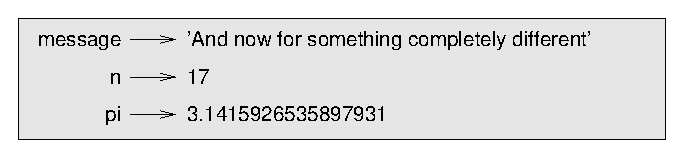
\includegraphics{figs/state2.eps}}
\afterfig

To display the value of a variable, you can use a print statement:

\beforeverb
\begin{verbatim}
>>> print n
17
>>> print pi
3.14159265359
\end{verbatim}
\afterverb
%
The type of a variable is the type of the value it refers to.

\beforeverb
\begin{verbatim}
>>> type(message)
<type 'str'>
>>> type(n)
<type 'int'>
>>> type(pi)
<type 'float'>
\end{verbatim}
\afterverb
%

\section{Variable names and keywords}
\index{keyword}

Programmers generally choose names for their variables that
are meaningful---they document what the variable is used for.

Variable names can be arbitrarily long.  They can contain
both letters and numbers, but they have to begin with a letter.
It is legal to use uppercase letters, but it is a good idea
to begin variable names with a lowercase letter (you'll
see why later).

The underscore character (\verb"_") can appear in a name.
It is often used in names with multiple words, such as
\verb"my_name" or \verb"airspeed_of_unladen_swallow".

\index{underscore character}

If you give a variable an illegal name, you get a syntax error:

\beforeverb
\begin{verbatim}
>>> 76trombones = 'big parade'
SyntaxError: invalid syntax
>>> more@ = 1000000
SyntaxError: invalid syntax
>>> class = 'Advanced Theoretical Zymurgy'
SyntaxError: invalid syntax
\end{verbatim}
\afterverb
%
{\tt 76trombones} is illegal because it does not begin with a letter.
{\tt more@} is illegal because it contains an illegal character, {\tt
@}.  But what's wrong with {\tt class}?

It turns out that {\tt class} is one of Python's {\bf keywords}.  The
interpreter uses keywords to recognize the structure of the program,
and they cannot be used as variable names.

\index{keyword}

Python reserves 31 keywords\footnote{In Python 3.0, {\tt exec} is no
longer a keyword, but {\tt nonlocal} is.} for its use:

\beforeverb
\begin{verbatim}
and       del       from      not       while    
as        elif      global    or        with     
assert    else      if        pass      yield    
break     except    import    print              
class     exec      in        raise              
continue  finally   is        return             
def       for       lambda    try
\end{verbatim}
\afterverb
%
You might want to keep this list handy.  If the interpreter complains
about one of your variable names and you don't know why, see if it
is on this list.

\section{Statements}

A {\bf statement} is a unit of code that the Python interpreter can
execute.  We have seen two kinds of statements: print
and assignment.

\index{statement}
\index{interactive mode}
\index{script mode}

When you type a statement in interactive mode, the interpreter
executes it and displays the result, if there is one.

A script usually contains a sequence of statements.  If there
is more than one statement, the results appear one at a time
as the statements execute.

For example, the script

\beforeverb
\begin{verbatim}
print 1
x = 2
print x
\end{verbatim}
\afterverb
%
produces the output

\beforeverb
\begin{verbatim}
1
2
\end{verbatim}
\afterverb
%
The assignment statement produces no output.


\section{Operators and operands}
\index{operator, arithmetic}
\index{arithmetic operator}
\index{operand}
\index{expression}

{\bf Operators} are special symbols that represent computations like
addition and multiplication.  The values the operator is applied to
are called {\bf operands}.

The operators {\tt +}, {\tt -}, {\tt *}, {\tt /} and {\tt **}
perform addition, subtraction, multiplication, division and
exponentiation, as in the following examples:

\beforeverb
\begin{verbatim}
20+32   hour-1   hour*60+minute   minute/60   5**2   (5+9)*(15-7)
\end{verbatim}
\afterverb
%
The division operator might not do what you expect:

\beforeverb
\begin{verbatim}
>>> minute = 59
>>> minute/60
0
\end{verbatim}
\afterverb
%
The value of {\tt minute} is 59, and in conventional arithmetic 59
divided by 60 is 0.98333, not 0.  The reason for the discrepancy is
that Python is performing {\bf floor division}\footnote{In Python 3.0,
the result of this division is a {\tt float}.  
In Python 3.0, the new operator
{\tt //} performs integer division.}.

\index{Python 3.0}
\index{floor division}
\index{floating-point division}
\index{division!floor}
\index{division!floating-point}

When both of the operands are integers, the result is also an
integer; floor division chops off the fraction
part, so in this example it rounds down to zero.

If either of the operands is a floating-point number, Python performs
floating-point division, and the result is a {\tt float}:

\beforeverb
\begin{verbatim}
>>> minute/60.0
0.98333333333333328
\end{verbatim}
\afterverb


\section{Expressions}

An {\bf expression} is a combination of values, variables, and operators.
A value all by itself is considered an expression, and so is
a variable, so the following are all legal expressions
(assuming that the variable {\tt x} has been assigned a value):

\index{expression}
\index{evaluate}

\beforeverb
\begin{verbatim}
17
x
x + 17
\end{verbatim}
\afterverb
%
If you type an expression in interactive mode, the interpreter
{\bf evaluates} it and displays the result:

\beforeverb
\begin{verbatim}
>>> 1 + 1
2
\end{verbatim}
\afterverb
%
But in a script, an expression all by itself doesn't
do anything!  This is a common
source of confusion for beginners.

\begin{ex}
Type the following statements in the Python interpreter to see
what they do:

\beforeverb
\begin{verbatim}
5
x = 5
x + 1
\end{verbatim}
\afterverb
%
\end{ex}


\section{Order of operations}
\index{order of operations}
\index{rules of precedence}
\index{PEMDAS}

When more than one operator appears in an expression, the order of
evaluation depends on the {\bf rules of precedence}.  For
mathematical operators, Python follows mathematical convention.
The acronym {\bf PEMDAS} is a useful way to
remember the rules:

\index{parentheses!overriding precedence}

\begin{itemize}

\item {\bf P}arentheses have the highest precedence and can be used 
to force an expression to evaluate in the order you want. Since
expressions in parentheses are evaluated first, {\tt 2 * (3-1)} is 4,
and {\tt (1+1)**(5-2)} is 8. You can also use parentheses to make an
expression easier to read, as in {\tt (minute * 100) / 60}, even
if it doesn't change the result.

\item {\bf E}xponentiation has the next highest precedence, so
{\tt 2**1+1} is 3, not 4, and {\tt 3*1**3} is 3, not 27.

\item {\bf M}ultiplication and {\bf D}ivision have the same precedence,
which is higher than {\bf A}ddition and {\bf S}ubtraction, which also
have the same precedence.  So {\tt 2*3-1} is 5, not 4, and
{\tt 6+4/2} is 8, not 5.

\item Operators with the same precedence are evaluated from left to 
right.  So in the expression {\tt 5-3-1} is 1, not 3 because the
{\tt 5-3} happens first and then {\tt 1} is subtracted from {\tt 2}.

\end{itemize}

When in doubt always put parentheses in your expressions to make sure
the computations are performed in the order you intend.

\section{Modulus operator}

\index{modulus operator}
\index{operator!modulus}

The {\bf modulus operator} works on integers and yields the remainder
when the first operand is divided by the second.  In Python, the
modulus operator is a percent sign (\verb"%").  The syntax is the same
as for other operators:

\beforeverb
\begin{verbatim}
>>> quotient = 7 / 3
>>> print quotient
2
>>> remainder = 7 % 3
>>> print remainder
1
\end{verbatim}
\afterverb
%
So 7 divided by 3 is 2 with 1 left over.

The modulus operator turns out to be surprisingly useful.  For
example, you can check whether one number is divisible by another---if
{\tt x \% y} is zero, then {\tt x} is divisible by {\tt y}.

\index{divisibility}

Also, you can extract the right-most digit
or digits from a number.  For example, {\tt x \% 10} yields the
right-most digit of {\tt x} (in base 10).  Similarly {\tt x \% 100}
yields the last two digits.



\section{String operations}
\index{string!operation}
\index{operator!string}

The {\tt +} operator works with strings, but it
is not addition in the mathematical sense. Instead it performs
{\bf concatenation}, which means joining the strings by
linking them end-to-end.  For example:

\index{concatenation}

\beforeverb
\begin{verbatim}
first = 'throat'
second = 'warbler'
print first + second
\end{verbatim}
\afterverb
%
The output of this program is {\tt throatwarbler}.

\section{Asking the user for input}
\index{keyboard input}

Sometimes we would like to take the value for a variable from the user
via their keyboard.
Python provides a built-in function called \verb"raw_input" that gets
input from the keyboard\footnote{In Python 3.0, this function is named
  {\tt input}.}.  When this function is called, the program stops and
waits for the user to type something.  When the user presses {\sf
  Return} or {\sf Enter}, the program resumes and \verb"raw_input"
returns what the user typed as a string.

\index{Python 3.0}
\index{raw\_input function}
\index{function!raw\_input}

\beforeverb
\begin{verbatim}
>>> input = raw_input()
Some silly stuff
>>> print input
Some silly stuff
\end{verbatim}
\afterverb
%
Before getting input from the user, it is a good idea to print a
prompt telling the user what to input.  \verb"raw_input" can take a
prompt as an argument:

\index{prompt}

\beforeverb
\begin{verbatim}
>>> name = raw_input('What...is your name?\n')
What...is your name?
Arthur, King of the Britons!
>>> print name
Arthur, King of the Britons!
\end{verbatim}
\afterverb
%
The sequence \verb"\n" at the end of the prompt represents a {\bf newline},
which is a special character that causes a line break.
That's why the user's input appears below the prompt.

\index{newline}

If you expect the user to type an integer, you can try to convert
the return value to {\tt int} using the {\tt int()} function:

\beforeverb
\begin{verbatim}
>>> prompt = 'What...is the airspeed velocity of an unladen swallow?\n'
>>> speed = raw_input(prompt)
What...is the airspeed velocity of an unladen swallow?
17
>>> int(speed)
17
>>> int(speed) + 5
22
\end{verbatim}
\afterverb
%
But if the user types something other than a string of digits,
you get an error:

\beforeverb
\begin{verbatim}
>>> speed = raw_input(prompt)
What...is the airspeed velocity of an unladen swallow?
What do you mean, an African or a European swallow?
>>> int(speed)
ValueError: invalid literal for int()
\end{verbatim}
\afterverb
%
We will see how to handle this kind of error later.

\index{ValueError}
\index{exception!ValueError}


\section{Comments}
\index{comment}

As programs get bigger and more complicated, they get more difficult
to read.  Formal languages are dense, and it is often difficult to
look at a piece of code and figure out what it is doing, or why.

For this reason, it is a good idea to add notes to your programs to explain
in natural language what the program is doing.  These notes are called
{\bf comments}, and they start with the \verb"#" symbol:

\beforeverb
\begin{verbatim}
# compute the percentage of the hour that has elapsed
percentage = (minute * 100) / 60
\end{verbatim}
\afterverb
%
In this case, the comment appears on a line by itself.  You can also put
comments at the end of a line:

\beforeverb
\begin{verbatim}
percentage = (minute * 100) / 60     # percentage of an hour
\end{verbatim}
\afterverb
%
Everything from the {\tt \#} to the end of the line is ignored---it
has no effect on the program.

Comments are most useful when they document non-obvious features of
the code.  It is reasonable to assume that the reader can figure out
\emph{what} the code does; it is much more useful to explain \emph{why}.

This comment is redundant with the code and useless:

\beforeverb
\begin{verbatim}
v = 5     # assign 5 to v
\end{verbatim}
\afterverb
%
This comment contains useful information that is not in the code:

\beforeverb
\begin{verbatim}
v = 5     # velocity in meters/second. 
\end{verbatim}
\afterverb
%
Good variable names can reduce the need for comments, but
long names can make complex expressions hard to read, so there is
a tradeoff.

\section{Choosing mnemonic variable names}

\index{mnemonic}

As long as you follow the simple rules of variable naming, and avoid
reserved words, you have a lot of choice when you name your variables.
In the beginning, this choice can be confusing both when you read a 
program and when you write your own programs.  For example, the
following three programs are identical in terms of what they accomplish,
but very different when you read them and try to understand them.

\beforeverb
\begin{verbatim}
a = 35.0
b = 12.50
c = a * b
print c

hours = 35.0
rate = 12.50
pay = hours * rate
print pay

x1q3z9ahd = 35.0
x1q3z9afd = 12.50
x1q3p9afd = x1q3z9ahd * x1q3z9afd
print x1q3p9afd
\end{verbatim}
\afterverb
%
The Python interpreter sees all three of these programs as \emph{exactly the 
same} but humans see and understand these programs quite differently.  
Humans will most quickly understand the {\bf intent} 
of the second program because the 
programmer has chosen variable names that reflect the intent of the programmer
regarding what data will be stored in each variable.

We call these wisely-chosen variable names ``mnemonic variable names''.  The
word \emph{mnemonic}\footnote{See 
\url{http://en.wikipedia.org/wiki/Mnemonic}
for an extended description of the word ``mnemonic''.} 
means ``memory aid''.
We choose mnemonic variable names to help us remember why we created the variable
in the first place.

While this all sounds great, and it is a very good idea to use mnemonic variable
names, mnemonic variable names can get in the way of a beginning programmer's 
ability to parse and understand code.  This is because beginning programmers 
have not yet memorized the reserved words (there are only 31 of them) and sometimes
variables which have names that are too descriptive start to look like 
part of the language and not just well-chosen variable names.

Take a quick look at the following Python sample code which loops through some data. 
We will cover loops soon, but for now try to just puzzle through what this means:

\beforeverb
\begin{verbatim}
for word in words:
    print word
\end{verbatim}
\afterverb
%
What is happening here?  Which of the tokens (for, word, in, etc.) are reserved words
and which are just variable names?  Does Python understand at a fundamental level 
the notion of words?  Beginning programmers have 
trouble separating what parts of the
code \emph{must} be the same as this example and what parts of the code are simply
choices made by the programmer.

The following code is equivalent to the above code:

\beforeverb
\begin{verbatim}
for slice in pizza:
    print slice
\end{verbatim}
\afterverb
%
It is easier for the beginning programmer to look at this code and know which 
parts are reserved words defined by Python and which parts are simply variable
names chosen by the programmer.  It is pretty clear that Python has no fundamental
understanding of pizza and slices and the fact that a pizza consists of a set
of one or more slices.

But if our program is truly about reading data and looking for words in the data,
{\tt pizza} and {\tt slice} are very un-mnemonic variable names.  Choosing them 
as variable names distracts from the meaning of the program.

After a pretty short period of time, you will know the most common reserved words
and you will start to see the reserved words jumping out at you:

{\tt {\bf for} word {\bf in} words{\bf :}\\
\verb"    "{\bf print} word }

The parts of the code that are defined by 
Python ({\tt for}, {\tt in}, {\tt print}, and {\tt :}) are in bold
and the programmer chosen variables ({\tt word} and {\tt words}) are not in bold.  
Many text editors are aware of Python
syntax and will color reserved words differently to give you clues to keep 
your variables and reserved words separate.
After a while you will begin to read Python and quickly determine what
is a variable and what is a reserved word.

\section{Debugging}
\index{debugging}

At this point the syntax error you are most likely to make is
an illegal variable name, like {\tt class} and {\tt yield}, which
are keywords, or \verb"odd~job" and \verb"US$", which contain
illegal characters.

\index{syntax error}
\index{error!syntax}

If you put a space in a variable name, Python thinks it is two
operands without an operator:

\beforeverb
\begin{verbatim}
>>> bad name = 5
SyntaxError: invalid syntax
\end{verbatim}
\afterverb
%
For syntax errors, the error messages don't help much.
The most common messages are {\tt SyntaxError: invalid syntax} and
{\tt SyntaxError: invalid token}, neither of which is very informative.

\index{error message}
\index{use before def}
\index{exception}
\index{runtime error}
\index{error!runtime}

The runtime error you are most likely to make is a ``use before
def;'' that is, trying to use a variable before you have assigned
a value.  This can happen if you spell a variable name wrong:

\beforeverb
\begin{verbatim}
>>> principal = 327.68
>>> interest = principle * rate
NameError: name 'principle' is not defined
\end{verbatim}
\afterverb
%
Variables names are case sensitive, so {\tt LaTeX} is not the
same as {\tt latex}.

\index{case-sensitivity, variable names}
\index{semantic error}
\index{error!semantic}

At this point the most likely cause of a semantic error is
the order of operations.  For example, to evaluate $\frac{1}{2 \pi}$,
you might be tempted to write

\beforeverb
\begin{verbatim}
>>> 1.0 / 2.0 * pi
\end{verbatim}
\afterverb
%
But the division happens first, so you would get $\pi / 2$, which
is not the same thing!  There is no way for Python
to know what you meant to write, so in this case you don't
get an error message; you just get the wrong answer.

\index{order of operations}


\section{Glossary}

\begin{description}

\item[assignment:]  A statement that assigns a value to a variable.
\index{assignment}

\item[concatenate:]  To join two operands end-to-end.
\index{concatenation}

\item[comment:]  Information in a program that is meant for other
programmers (or anyone reading the source code) and has no effect on the
execution of the program.
\index{comment}

\item[evaluate:]  To simplify an expression by performing the operations
in order to yield a single value.

\item[expression:]  A combination of variables, operators, and values that
represents a single result value.
\index{expression}

\item[floating-point:] A type that represents numbers with fractional
parts.
\index{floating-point}

\item[floor division:] The operation that divides two numbers and chops off
the fraction part.
\index{floor division}

\item[integer:] A type that represents whole numbers.
\index{integer}

\item[keyword:]  A reserved word that is used by the compiler to parse a
program; you cannot use keywords like {\tt if}, {\tt  def}, and {\tt while} as
variable names.
\index{keyword}

\item[mnemonic:] A memory aid. We often give variables mnemonic names
to help us remember what is stored in the variable.
\index{mnemonic}

\item[modulus operator:]  An operator, denoted with a percent sign
({\tt \%}), that works on integers and yields the remainder when one
number is divided by another.
\index{modulus operator}
\index{operator!modulus}

\item[operand:]  One of the values on which an operator operates.
\index{operand}

\item[operator:]  A special symbol that represents a simple computation like
addition, multiplication, or string concatenation.
\index{operator}

\item[rules of precedence:]  The set of rules governing the order in which
expressions involving multiple operators and operands are evaluated.
\index{rules of precedence}
\index{precedence}

\item[state diagram:]  A graphical representation of a set of variables and the
values they refer to.
\index{state diagram}

\item[statement:]  A section of code that represents a command or action.  So
far, the statements we have seen are assignments and print statements.
\index{statement}

\item[string:] A type that represents sequences of characters.
\index{string}

\item[type:] A category of values.  The types we have seen so far
are integers (type {\tt int}), floating-point numbers (type {\tt
float}), and strings (type {\tt str}).
\index{type}

\item[value:]  One of the basic units of data, like a number or string, 
that a program manipulates.
\index{value}

\item[variable:]  A name that refers to a value.
\index{variable}

\end{description}

\section{Exercises}

\begin{ex}
Write a program that uses  \verb"raw_input" to prompt a user for their name 
and then welcomes them.

\begin{verbatim}
Enter your name: Chuck
Hello Chuck
\end{verbatim}

\end{ex}

\begin{ex}
Write a program to prompt the user for hours and rate per hour to compute
gross pay.
\begin{verbatim}
Enter Hours: 35
Enter Rate: 2.75
Pay: 96.25
\end{verbatim}
\end{ex}
%
We won't worry about making sure our pay has exactly two digits after
the decimal place for now.  If you want, you can play with the 
built-in Python {\tt round} function to properly round the resulting pay
to two decimal places.

\begin{ex}
Assume that we execute the following assignment statements:

\begin{verbatim}
width = 17
height = 12.0
\end{verbatim}

For each of the following expressions, write the value of the
expression and the type (of the value of the expression).

\begin{enumerate}

\item {\tt width/2}

\item {\tt width/2.0}

\item {\tt height/3}

\item {\tt 1 + 2 * 5}

\end{enumerate}

Use the Python interpreter to check your answers.
\end{ex}

\begin{ex}
Write a program which prompts the user for a Celsius temperature,
convert the temperature to Fahrenheit and print out the converted
temperature.
\end{ex}


\chapter{Conditional execution}

\section{Boolean expressions}
\index{boolean expression}
\index{expression!boolean}
\index{logical operator}
\index{operator!logical}

A {\bf boolean expression} is an expression that is either true
or false.  The following examples use the 
operator {\tt ==}, which compares two operands and produces
{\tt True} if they are equal and {\tt False} otherwise:

\beforeverb
\begin{verbatim}
>>> 5 == 5
True
>>> 5 == 6
False
\end{verbatim}
\afterverb
%
{\tt True} and {\tt False} are special
values that belong to the type {\tt bool}; they are not strings:

\index{True special value}
\index{False special value}
\index{special value!True}
\index{special value!False}
\index{bool type}
\index{type!bool}

\beforeverb
\begin{verbatim}
>>> type(True)
<type 'bool'>
>>> type(False)
<type 'bool'>
\end{verbatim}
\afterverb
%
The {\tt ==} operator is one of the {\bf comparison operators}; the
others are:

\beforeverb
\begin{verbatim}
      x != y               # x is not equal to y
      x > y                # x is greater than y
      x < y                # x is less than y
      x >= y               # x is greater than or equal to y
      x <= y               # x is less than or equal to y
      x is y               # x is the same as y
      x is not y           # x is not the same as y
\end{verbatim}
\afterverb
%
Although these operations are probably familiar to you, the Python
symbols are different from the mathematical symbols.  A common error
is to use a single equal sign ({\tt =}) instead of a double equal sign
({\tt ==}).  Remember that {\tt =} is an assignment operator and
{\tt ==} is a comparison operator.   There is no such thing as
{\tt =<} or {\tt =>}.

\index{comparison operator}
\index{operator!comparison}


\section {Logical operators}
\index{logical operator}
\index{operator!logical}

There are three {\bf logical operators}: {\tt and}, {\tt
or}, and {\tt not}.  The semantics (meaning) of these operators is
similar to their meaning in English.  For example,

{\tt x > 0 and x < 10} 

is true only if {\tt x} is greater than 0
\emph{and} less than 10.

\index{and operator}
\index{or operator}
\index{not operator}
\index{operator!and}
\index{operator!or}
\index{operator!not}

{\tt n\%2 == 0 or n\%3 == 0} is true if \emph{either} of the conditions
is true, that is, if the number is divisible by 2 \emph{or} 3.

Finally, the {\tt not} operator negates a boolean
expression, so {\tt not (x > y)} is true if {\tt x > y} is false,
that is, if {\tt x} is less than or equal to {\tt y}.

Strictly speaking, the operands of the logical operators should be
boolean expressions, but Python is not very strict.
Any nonzero number is interpreted as ``true.''

\beforeverb
\begin{verbatim}
>>> 17 and True
True
\end{verbatim}
\afterverb
%
This flexibility can be useful, but there are some subtleties to
it that might be confusing.  You might want to avoid it (unless
you know what you are doing).

\section{Conditional execution}
\label{conditional execution}

\index{conditional statement}
\index{statement!conditional}
\index{if statement}
\index{statement!if}
\index{conditional execution}

In order to write useful programs, we almost always need the ability
to check conditions and change the behavior of the program
accordingly.  {\bf Conditional statements} give us this ability.  The
simplest form is the {\tt if} statement:

\beforeverb
\begin{verbatim}
if x > 0 :
    print 'x is positive'
\end{verbatim}
\afterverb
%
The boolean expression after the {\tt if} statement is
called the {\bf condition}.  We end the {\tt if} 
statement with a colon character (:) and the line(s) 
after the if statement are indented.  

\beforefig
\centerline{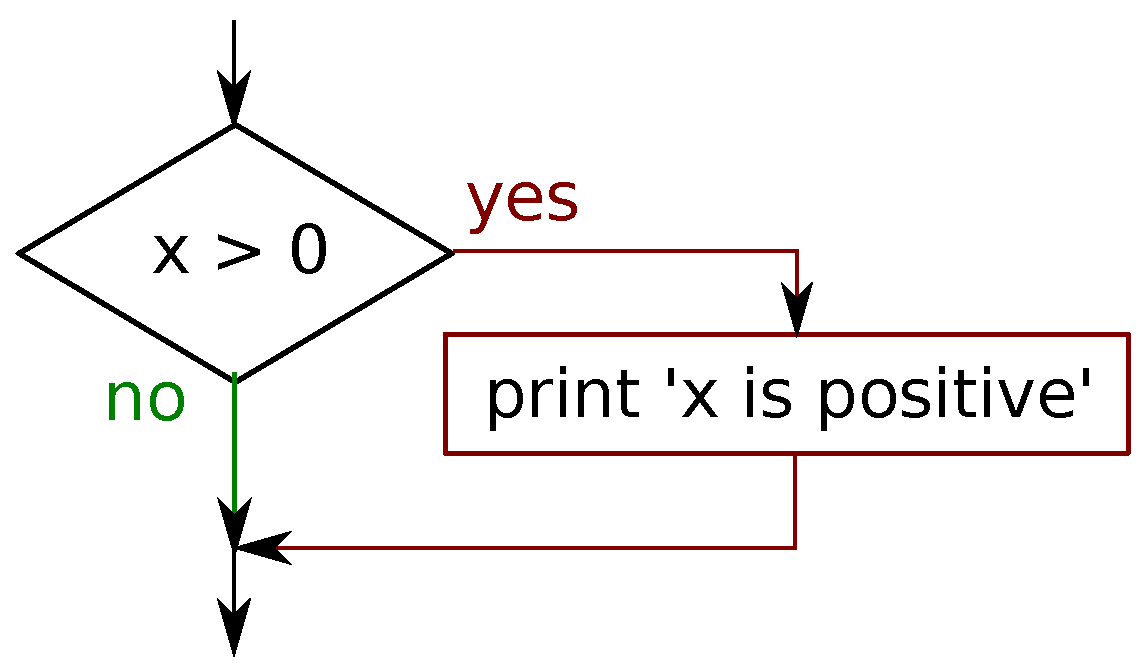
\includegraphics[height=1.75in]{figs2/if.eps}}
\afterfig

If the logical condition is true, then the indented
statement gets executed.  If the logical condition is 
false, the indented statement is skipped.

\index{condition}
\index{compound statement}
\index{statement!compound}

{\tt if} statements have the same structure as function definitions
or {\tt for} loops.  The statement consists of a header line
that ends with the colon character (:) 
followed by an indented block.  Statements like this are
called {\bf compound statements} because they stretch 
across more than one line.

There is no limit on the number of statements that can appear in
the body, but there has to be at least one.
Occasionally, it is useful to have a body with no statements (usually
as a place keeper for code you haven't written yet).  In that
case, you can use the {\tt pass} statement, which does nothing.

\index{pass statement}
\index{statement!pass}

\beforeverb
\begin{verbatim}
if x < 0 :
    pass          # need to handle negative values!
\end{verbatim}
\afterverb
%

\section{Alternative execution}
\label{alternative execution}

\index{alternative execution}
\index{else keyword}
\index{keyword!else}

A second form of the {\tt if} statement is {\bf alternative execution},
in which there are two possibilities and the condition determines
which one gets executed.  The syntax looks like this:

\beforeverb
\begin{verbatim}
if x%2 == 0 :
    print 'x is even'
else :
    print 'x is odd'
\end{verbatim}
\afterverb
%
If the remainder when {\tt x} is divided by 2 is 0, then we
know that {\tt x} is even, and the program displays a message to that
effect.  If the condition is false, the second set of statements is
executed.  

\beforefig
\centerline{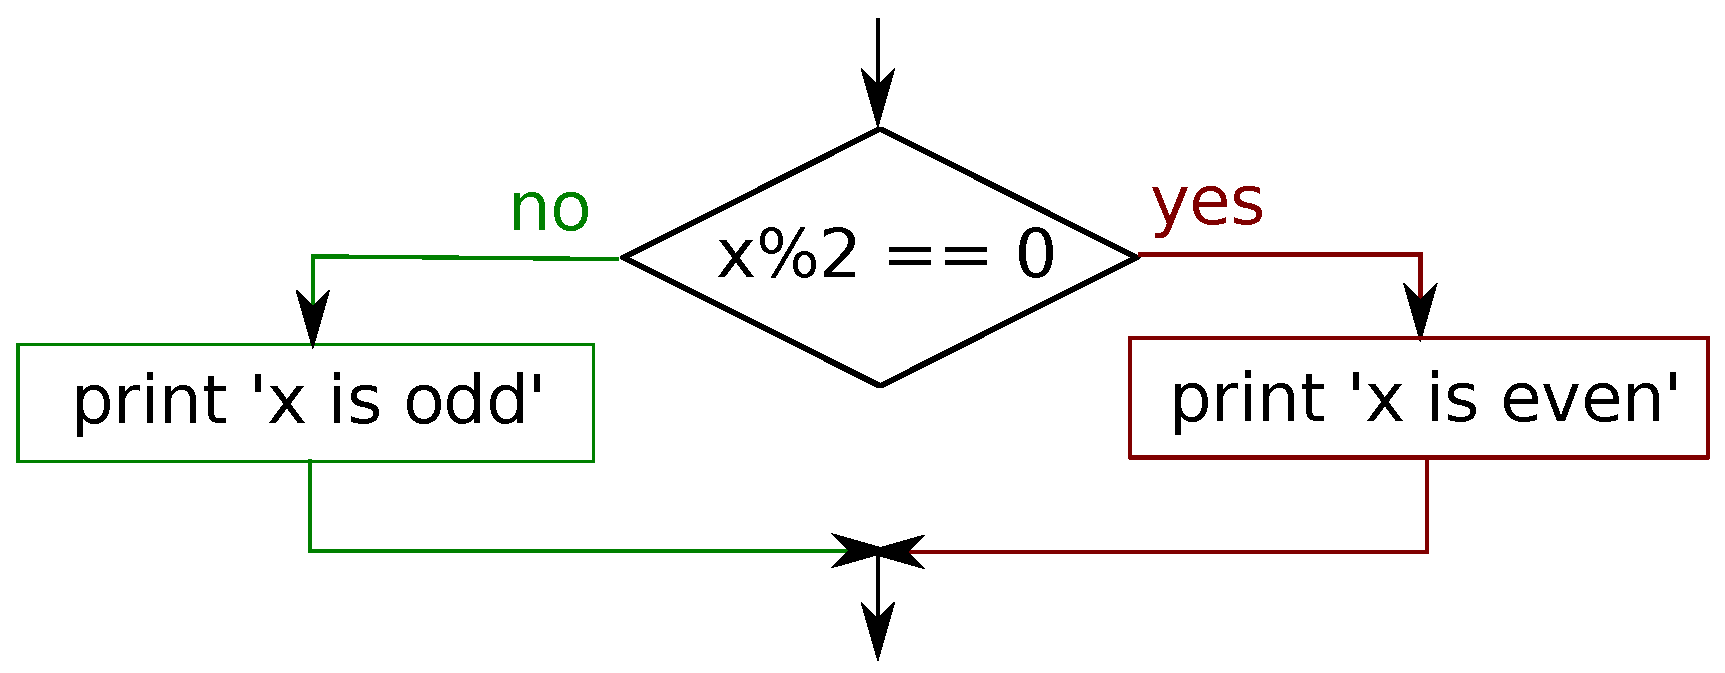
\includegraphics[height=1.75in]{figs2/if-else.eps}}
\afterfig

Since the condition must be true or false, exactly one of
the alternatives will be executed.  The alternatives are called
{\bf branches}, because they are branches in the flow of execution.

\index{branch}



\section{Chained conditionals}
\index{chained conditional}
\index{conditional!chained}

Sometimes there are more than two possibilities and we need more than
two branches.  One way to express a computation like that is a {\bf
chained conditional}:

\beforeverb
\begin{verbatim}
if x < y:
    print 'x is less than y'
elif x > y:
    print 'x is greater than y'
else:
    print 'x and y are equal'
\end{verbatim}
\afterverb
%
{\tt elif} is an abbreviation of ``else if.''  Again, exactly one
branch will be executed.  

\beforefig
\centerline{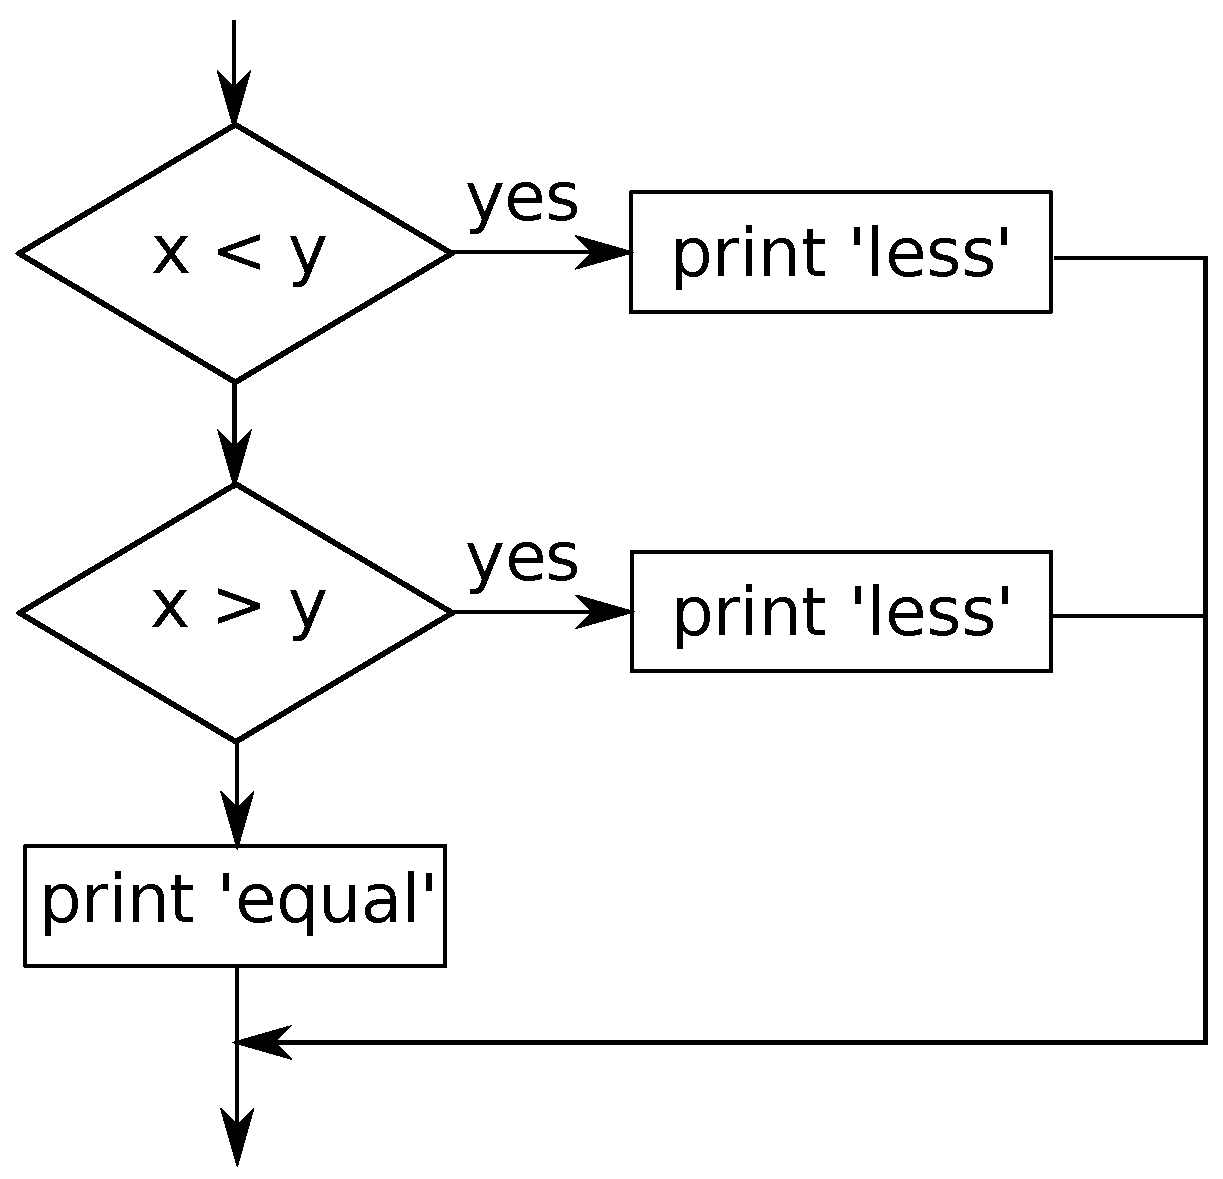
\includegraphics[height=3.00in]{figs2/elif.eps}}
\afterfig

There is no limit on the number of {\tt
elif} statements.  If there is an {\tt else} clause, it has to be
at the end, but there doesn't have to be one.

\index{elif keyword}
\index{keyword!elif}


\beforeverb
\begin{verbatim}
if choice == 'a':
    print 'Bad guess'
elif choice == 'b':
    print 'Good guess'
elif choice == 'c':
    print 'Close, but not correct'
\end{verbatim}
\afterverb
%
Each condition is checked in order.  If the first is false,
the next is checked, and so on.  If one of them is
true, the corresponding branch executes, and the statement
ends.  Even if more than one condition is true, only the
first true branch executes.  


\section{Nested conditionals}
\index{nested conditional}
\index{conditional!nested}

One conditional can also be nested within another.  We could have
written the trichotomy example like this:

\beforeverb
\begin{verbatim}
if x == y:
    print 'x and y are equal'
else:
    if x < y:
        print 'x is less than y'
    else:
        print 'x is greater than y'
\end{verbatim}
\afterverb
%
The outer conditional contains two branches.  The
first branch contains a simple statement.  The second branch
contains another {\tt if} statement, which has two branches of its
own.  Those two branches are both simple statements,
although they could have been conditional statements as well.

\beforefig
\centerline{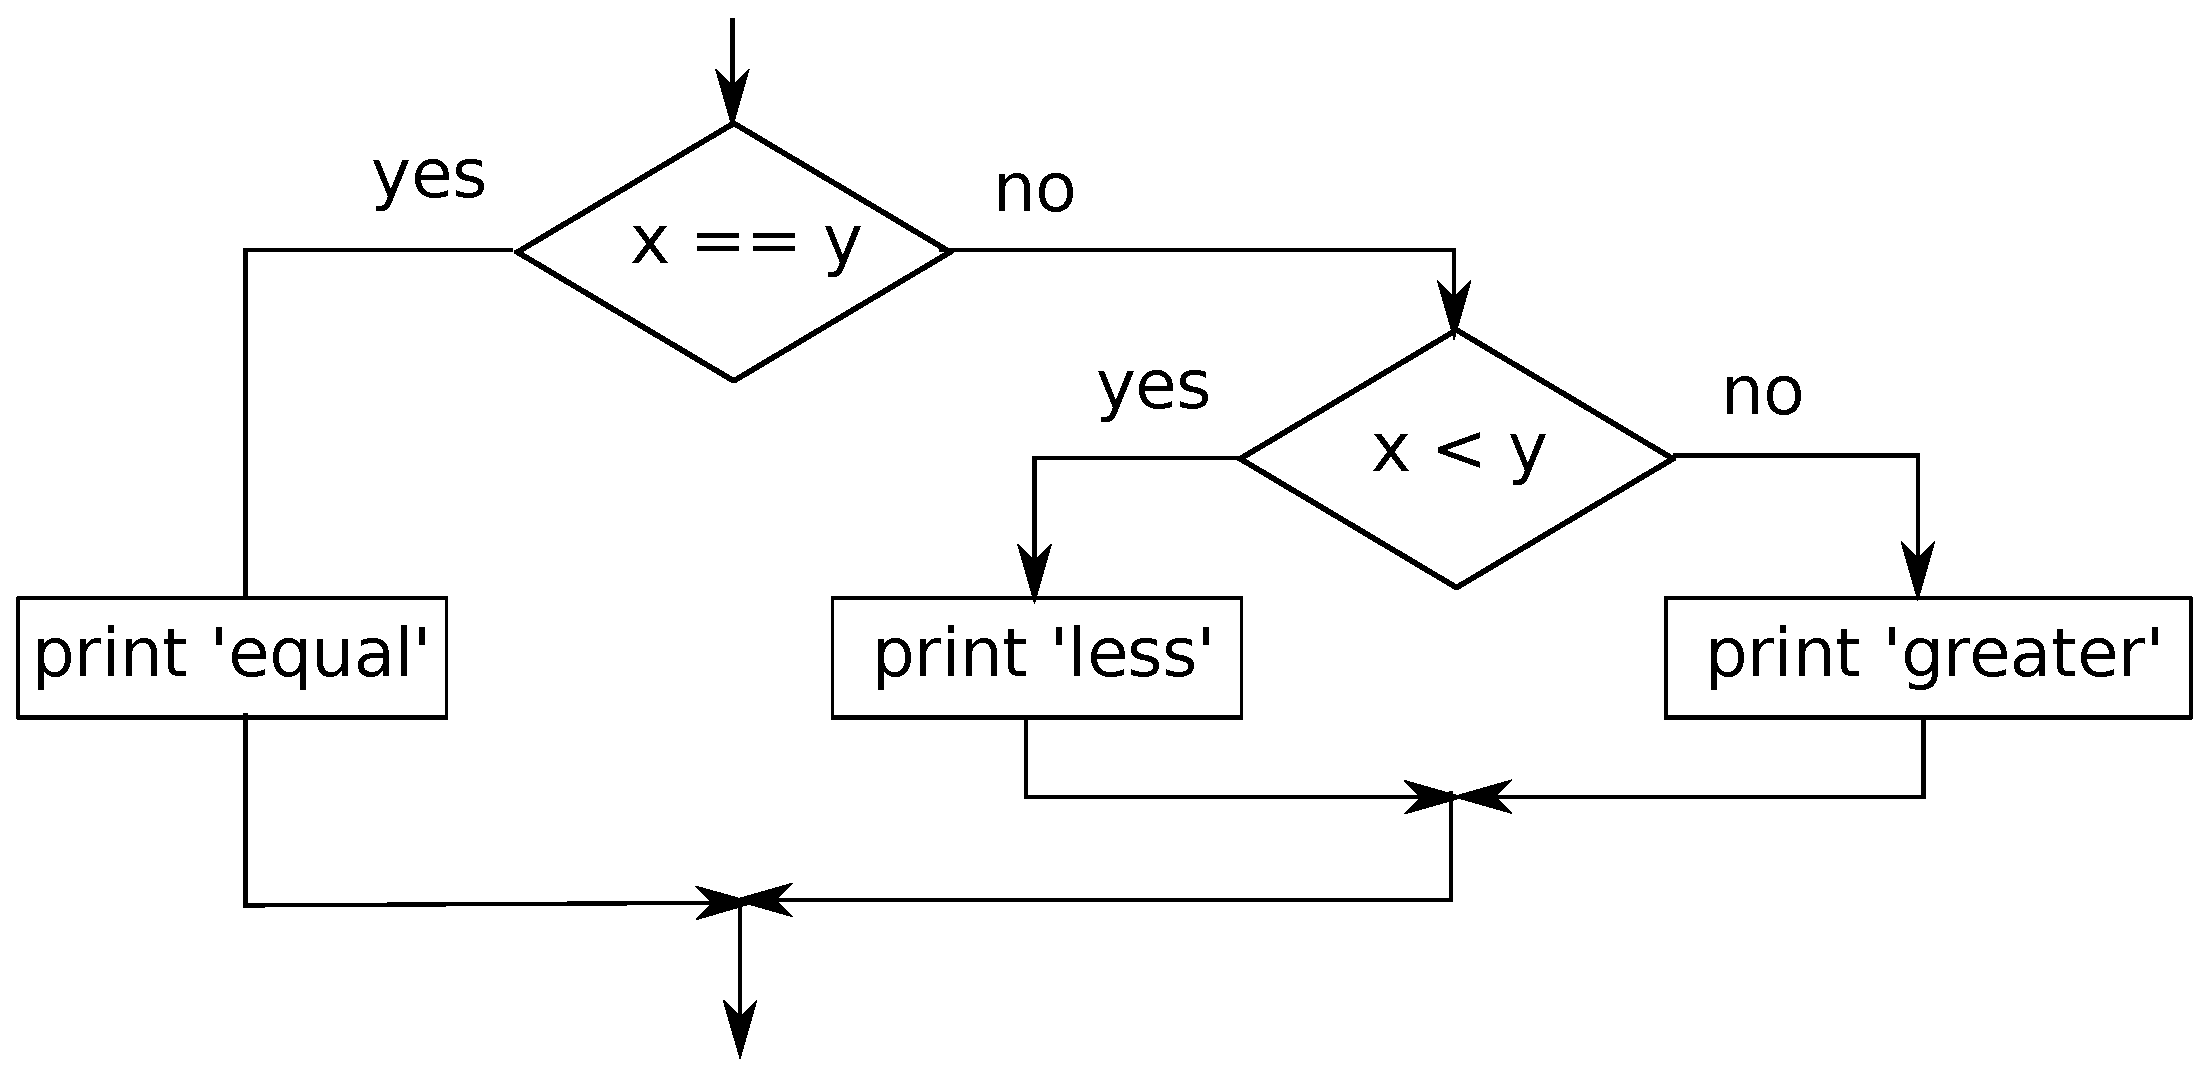
\includegraphics[height=2.50in]{figs2/nested.eps}}
\afterfig

Although the indentation of the statements makes the structure
apparent, {\bf nested conditionals} become difficult to read very
quickly. In general, it is a good idea to avoid them when you can.

Logical operators often provide a way to simplify nested conditional
statements.  For example, we can rewrite the following code using a
single conditional:

\beforeverb
\begin{verbatim}
if 0 < x:
    if x < 10:
        print 'x is a positive single-digit number.'
\end{verbatim}
\afterverb
%
The {\tt print} statement is executed only if we make it past both
conditionals, so we can get the same effect with the {\tt and} operator:

\beforeverb
\begin{verbatim}
if 0 < x and x < 10:
    print 'x is a positive single-digit number.'
\end{verbatim}
\afterverb


\section{Catching exceptions using try and except}
\label{catch1}

Earlier we saw a code segment where we used the \verb"raw_input" and
{\tt int} functions to read and parse an integer number entered by
the user.  We also saw how treacherous doing this could be:

\beforeverb
\begin{verbatim}
>>> speed = raw_input(prompt)
What...is the airspeed velocity of an unladen swallow?
What do you mean, an African or a European swallow?
>>> int(speed)
ValueError: invalid literal for int()
>>>
\end{verbatim}
\afterverb
%
When we are executing these statements in the Python interpreter, 
we get a new prompt from the interpreter, think ``oops'' and move 
on to our next statement.  

However if this code is placed in a 
Python script and this error occurs, your script immediately 
stops in its tracks with a traceback.  
It does not execute the following statement. 
\index{traceback}

Here is a sample program to convert a Fahrenheit temperature 
to a Celsius temperature:
\index{fahrenheit}
\index{celsius}
\index{temperature conversion}

\beforeverb
\begin{verbatim}
inp = raw_input('Enter Fahrenheit Temperature:')
fahr = float(inp)
cel = (fahr - 32.0) * 5.0 / 9.0
print cel
\end{verbatim}
\afterverb
%
If we execute this code and give it invalid input, it simply fails
with an unfriendly error message:

\beforeverb
\begin{verbatim}
python fahren.py 
Enter Fahrenheit Temperature:72
22.2222222222

python fahren.py 
Enter Fahrenheit Temperature:fred
Traceback (most recent call last):
  File "fahren.py", line 2, in <module>
    fahr = float(inp)
ValueError: invalid literal for float(): fred
\end{verbatim}
\afterverb
%
There is a conditional execution structure built into 
Python to handle these types of expected and unexpected
errors called ``try / except''.  The idea of {\tt try}
and {\tt except} is that you know that some sequence
of instruction(s) may have a problem and you want to 
add some statements to be executed if an error occurs.
These extra statements (the except block) are ignored
if there is no error.

You can think of the {\tt try} and {\tt except} feature
in Python as an ``insurance policy'' on a sequence of
statements.

We can rewrite our temperature converter as follows:

\beforeverb
\begin{verbatim}
inp = raw_input('Enter Fahrenheit Temperature:')
try:
    fahr = float(inp)
    cel = (fahr - 32.0) * 5.0 / 9.0
    print cel
except:
    print 'Please enter a number'
\end{verbatim}
\afterverb
%

Python starts by executing the 
sequence of statements in the 
{\tt try} block.  If all goes
well, it skips the {\tt except} block and proceeds.  If an
exception occurs in the {\tt try} block, 
Python jumps out of the {\tt try} block and
executes the sequence of statements in the {\tt except} block.

\beforeverb
\begin{verbatim}
python fahren2.py 
Enter Fahrenheit Temperature:72
22.2222222222

python fahren2.py 
Enter Fahrenheit Temperature:fred
Please enter a number
\end{verbatim}
\afterverb
%

Handling an exception with a {\tt try} statement is called {\bf
catching} an exception.  In this example, the {\tt except} clause
prints an error message.  In general,
catching an exception gives you a chance to fix the problem, or try
again, or at least end the program gracefully.

\section{Short circuit evaluation of logical expressions}
\index{short circuit}

When Python is processing a logical expression such as 
{\tt x >= 2 and (x/y) > 2}, it evaluates the expression
from left-to-right.  Because of the definition of {\tt and},
if {\tt x} is less than 2, the expression {\tt x >= 2} is 
{\tt False} and so the whole expression is {\tt False} regardless
of whether {\tt (x/y) > 2} evaluates to {\tt True} or {\tt False}.

When Python detects that there is nothing to be gained by evaluating
the rest of a logical expression, it stops its evaluation and does
not do the computations in the rest of the logical expression.  
When the evaluation of a logical expression stops because the overall
value is already known, it is called {\bf short-circuiting} 
the evaluation.

\index{guardian pattern}
\index{pattern!guardian}
While this may seem like a fine point, the short circuit behavior
leads to a clever technique called the {\bf guardian pattern}.  
Consider the following code sequence in the Python interpreter:

\beforeverb
\begin{verbatim}
>>> x = 6 
>>> y = 2
>>> x >= 2 and (x/y) > 2
True
>>> x = 1 
>>> y = 0
>>> x >= 2 and (x/y) > 2
False
>>> x = 6
>>> y = 0
>>> x >= 2 and (x/y) > 2
Traceback (most recent call last):
  File "<stdin>", line 1, in <module>
ZeroDivisionError: integer division or modulo by zero
>>> 
\end{verbatim}
\afterverb
%
The third calculation failed because Python was evaluating {\tt (x/y)}
and {\tt y} was zero which causes a runtime error.  But the second example
did \emph{not} fail because the first part of the expression {\tt x >= 2} 
evaluated to {\tt False} so the {\tt (x/y)} was not ever executed 
due to the {\bf short circuit} rule and there was no error.

We can construct the logical expression to strategically place a {\bf guard}
evaluation just before the evaluation that might cause an error as follows:

\beforeverb
\begin{verbatim}
>>> x = 1
>>> y = 0
>>> x >= 2 and y != 0 and (x/y) > 2
False
>>> x = 6 
>>> y = 0
>>> x >= 2 and y != 0 and (x/y) > 2
False
>>> x >= 2 and (x/y) > 2 and y != 0
Traceback (most recent call last):
  File "<stdin>", line 1, in <module>
ZeroDivisionError: integer division or modulo by zero
>>>
\end{verbatim}
\afterverb
%
In the first logical expression, {\tt x >= 2} is {\tt False} so the evaluation
stops at the {\tt and}.  In the second logical expression {\tt x >= 2} is {\tt True}
but {\tt y != 0} is {\tt False} so we never reach {\tt (x/y)}.

In the third logical expression, the {\tt y != 0} is \emph{after} the 
{\tt (x/y) } calculation so the expression fails with an error.

In the second expression, we say that {\tt y != 0} acts as a {\bf guard}
to insure that we only execute {\tt (x/y)} if {\tt y} is non-zero.


\section{Debugging}
\label{whitespace}
\index{debugging}
\index{traceback}

The traceback Python displays when an error occurs contains
a lot of information, but it can be overwhelming, especially
when there are many frames on the stack.  The most
useful parts are usually:

\begin{itemize}

\item What kind of error it was, and

\item Where it occurred.

\end{itemize}

Syntax errors are usually easy to find, but there are a few
gotchas.  Whitespace errors can be tricky because spaces and
tabs are invisible and we are used to ignoring them.

\index{whitespace}

\beforeverb
\begin{verbatim}
>>> x = 5
>>>  y = 6
  File "<stdin>", line 1
    y = 6
    ^
SyntaxError: invalid syntax
\end{verbatim}
\afterverb
%
In this example, the problem is that the second line is indented by
one space.  But the error message points to {\tt y}, which is
misleading.  In general, error messages indicate where the problem was
discovered, but the actual error might be earlier in the code,
sometimes on a previous line.

\index{error!runtime}
\index{runtime error}

The same is true of runtime errors.  Suppose you are trying
to compute a signal-to-noise ratio in decibels.  The formula
is $SNR_{db} = 10 \log_{10} (P_{signal} / P_{noise})$.  In Python,
you might write something like this:

\beforeverb
\begin{verbatim}
import math
signal_power = 9
noise_power = 10
ratio = signal_power / noise_power
decibels = 10 * math.log10(ratio)
print decibels
\end{verbatim}
\afterverb
%
But when you run it, you get an error message\footnote{In Python 3.0,
  you no longer get an error message; the division operator performs
  floating-point division even with integer operands.}:

\index{exception!OverflowError}
\index{OverflowError}

\beforeverb
\begin{verbatim}
Traceback (most recent call last):
  File "snr.py", line 5, in ?
    decibels = 10 * math.log10(ratio)
OverflowError: math range error
\end{verbatim}
\afterverb
%
The error message indicates line 5, but there is nothing
wrong with that line.  To find the real error, it might be
useful to print the value of {\tt ratio}, which turns out to
be 0.  The problem is in line 4, because dividing two integers
does floor division.  The solution is to represent signal power
and noise power with floating-point values.

\index{floor division}
\index{division!floor}

In general, error messages tell you where the problem was discovered, 
but that is often not where it was caused.


\section{Glossary}

\begin{description}

\item[body:] The sequence of statements within a compound statement.
\index{body}

\item[boolean expression:]  An expression whose value is either 
{\tt True} or {\tt False}.
\index{boolean expression}
\index{expression!boolean}

\item[branch:] One of the alternative sequences of statements in
a conditional statement.
\index{branch}

\item[chained conditional:]  A conditional statement with a series
of alternative branches.
\index{chained conditional}
\index{conditional!chained}

\item[comparison operator:] One of the operators that compares
its operands: {\tt ==}, {\tt !=}, {\tt >}, {\tt <}, {\tt >=}, and {\tt <=}.

\item[conditional statement:]  A statement that controls the flow of
execution depending on some condition.
\index{conditional statement}
\index{statement!conditional}

\item[condition:] The boolean expression in a conditional statement
that determines which branch is executed.
\index{condition}

\item[compound statement:]  A statement that consists of a header
and a body.  The header ends with a colon (:).  The body is indented
relative to the header.
\index{compound statement}

\item[guardian pattern:] Where we construct a logical expression 
with additional
comparisons to take advantage of the short circuit behavior.
\index{guardian pattern}
\index{pattern!guardian}

\item[logical operator:] One of the operators that combines boolean
expressions: {\tt and}, {\tt or}, and {\tt not}.

\item[nested conditional:]  A conditional statement that appears
in one of the branches of another conditional statement.
\index{nested conditional}
\index{conditional!nested}

\item[traceback:]  A list of the functions that are executing,
printed when an exception occurs.
\index{traceback}

\item[short circuit:]  When Python is part-way through evaluating a 
logical expression and stops the evaluation because Python 
knows the final value for the expression 
without needing to evaluate the rest of the expression.
\index{short circuit}

\end{description}

\section{Exercises}

\begin{ex}
Rewrite your pay computation to give the employee 1.5 
times the hourly rate for 
hours worked above 40 hours.

\begin{verbatim}
Enter Hours: 45
Enter Rate: 10
Pay: 475.0
\end{verbatim}
\end{ex}

\begin{ex}
Rewrite your pay program using {\tt try} and {\tt except} 
so that your program handles non-numeric input gracefully
by printing a message and exiting the program.
The following shows two executions of the program:

\begin{verbatim}
Enter Hours: 20
Enter Rate: nine
Error, please enter numeric input

Enter Hours: forty
Error, please enter numeric input
\end{verbatim}
\end{ex}

\begin{ex}
Write a program to prompt for a score between 0.0 and 1.0.
If the score is out of range print an error.  If the score
is between 0.0 and 1.0, print a grade using the following 
table:

\begin{verbatim}
Score   Grade
>= 0.9     A
>= 0.8     B
>= 0.7     C
>= 0.6     D
< 0.6    F

Enter score: 0.95
A

Enter score: perfect
Bad score

Enter score: 10.0
Bad score

Enter score: 0.75
C

Enter score: 0.5
F
\end{verbatim}

Run the program repeatedly as shown above to test the 
various different values for input.
\end{ex}

\chapter{Functions}
\label{funcchap}

\section{Function calls}
\label{functionchap}
\index{function call}

In the context of programming, a {\bf function} is a named sequence of
statements that performs a computation.  When you define a function,
you specify the name and the sequence of statements.  Later, you can
``call'' the function by name.  
We have already seen one example of a {\bf function call}:

\beforeverb
\begin{verbatim}
>>> type(32)
<type 'int'>
\end{verbatim}
\afterverb
%
The name of the function is {\tt type}.  The expression in parentheses
is called the {\bf argument} of the function.  The argument is 
a value or variable that we are passing into the function as input 
to the function.  
The result, for the {\tt type} function, is the type of the argument.

\index{parentheses!argument in}

It is common to say that a function ``takes'' an argument and ``returns''
a result.  The result is called the {\bf return value}.

\index{argument}
\index{return value}

\section{Built-in functions}

Python provides a number of important built-in functions that
we can use without needing to provide the function definition.
In a sense, the creators or Python wrote a set of functions 
to solve common problems and included them in Python for us to use.

The {\tt max} and {\tt min} functions give us the largest and 
smallest values in a list, respectively:

\beforeverb
\begin{verbatim}
>>> max('Hello world')
'w'
>>> min('Hello world')
' '
>>>
\end{verbatim}
\afterverb
%
The {\tt max} function tells us the ``largest character'' in the 
string (which turns out to be the letter ``w'') and the {\tt min}
function shows us the smallest character which turns out to be a 
space.

Another very common built-in function is the {\tt len} function
which tells us how many items are in its argument. If the argument
to {\tt len} is a string, it returns the number of characters 
in the string.

\beforeverb
\begin{verbatim}
>>> len('Hello world')
11
>>>
\end{verbatim}
\afterverb
%
These functions are not limited to looking at strings, they can operate
on any set of values as we will see in later chapters.

\section{Type conversion functions}
\index{conversion!type}
\index{type conversion}

% from Elkner:
% comment on whether these things are _really_ functions?
% use max as an example of a built-in?

% my reply:
% they are on the list of ``built-in functions'' so I am
% willing to call them functions.

Python also provides built-in functions that convert values
from one type to another.  The {\tt int} function takes any value and
converts it to an integer, if it can, or complains otherwise:

\index{int function}
\index{function!int}

\beforeverb
\begin{verbatim}
>>> int('32')
32
>>> int('Hello')
ValueError: invalid literal for int(): Hello
\end{verbatim}
\afterverb
%
{\tt int} can convert floating-point values to integers, but it
doesn't round off; it chops off the fraction part:

\beforeverb
\begin{verbatim}
>>> int(3.99999)
3
>>> int(-2.3)
-2
\end{verbatim}
\afterverb
%
{\tt float} converts integers and strings to floating-point
numbers:

\index{float function}
\index{function!float}

\beforeverb
\begin{verbatim}
>>> float(32)
32.0
>>> float('3.14159')
3.14159
\end{verbatim}
\afterverb
%
Finally, {\tt str} converts its argument to a string:

\index{str function}
\index{function!str}

\beforeverb
\begin{verbatim}
>>> str(32)
'32'
>>> str(3.14159)
'3.14159'
\end{verbatim}
\afterverb
%

\section{Random numbers}

\index{random number}
\index{number, random}
\index{deterministic}
\index{pseudorandom}

Given the same inputs, most computer programs generate the same
outputs every time, so they are said to be {\bf deterministic}.
Determinism is usually a good thing, since we expect the same
calculation to yield the same result.  For some applications, though,
we want the computer to be unpredictable.  Games are an obvious
example, but there are more.

Making a program truly nondeterministic turns out to be not so easy,
but there are ways to make it at least seem nondeterministic.  One of
them is to use {\bf algorithms} that generate {\bf pseudorandom} numbers.
Pseudorandom numbers are not truly random because they are generated
by a deterministic computation, but just by looking at the numbers it
is all but impossible to distinguish them from random.

\index{random module}
\index{module!random}

The {\tt random} module provides functions that generate
pseudorandom numbers (which I will simply call ``random'' from
here on).

\index{random function}
\index{function!random}

The function {\tt random} returns a random float
between 0.0 and 1.0 (including 0.0 but not 1.0).  Each time you
call {\tt random}, you get the next number in a long series.  To see a
sample, run this loop:

\beforeverb
\begin{verbatim}
import random

for i in range(10):
    x = random.random()
    print x
\end{verbatim}
\afterverb
%
This program produces the following list of 10 random numbers
between 0.0 and up to but not including 1.0.
\beforeverb
\begin{verbatim}
0.301927091705
0.513787075867
0.319470430881
0.285145917252
0.839069045123
0.322027080731
0.550722110248
0.366591677812
0.396981483964
0.838116437404
\end{verbatim}
\afterverb
%
\begin{ex}
Run the program on your system and see what numbers you get.
Run the program more than once and see what numbers you get.
\end{ex}

The {\tt random} function is only one of many 
functions which handle random numbers.
The function {\tt randint} takes parameters {\tt low} and
{\tt high} and returns an integer between {\tt low} and
{\tt high} (including both).

\index{randint function}
\index{function!randint}

\beforeverb
\begin{verbatim}
>>> random.randint(5, 10)
5
>>> random.randint(5, 10)
9
\end{verbatim}
\afterverb
%
To choose an element from a sequence at random, you can use
{\tt choice}:

\index{choice function}
\index{function!choice}

\beforeverb
\begin{verbatim}
>>> t = [1, 2, 3]
>>> random.choice(t)
2
>>> random.choice(t)
3
\end{verbatim}
\afterverb
%
The {\tt random} module also provides functions to generate
random values from continuous distributions including
Gaussian, exponential, gamma, and a few more.

\section{Math functions}
\index{math function}
\index{function, math}

Python has a math {\bf module} that provides most of the familiar
mathematical functions.  
Before we can use the module, we have to import it:

\index{module}
\index{module object}
\beforeverb
\begin{verbatim}
>>> import math
\end{verbatim}
\afterverb
%
This statement creates a {\bf module object} named math.  If
you print the module object, you get some information about it:

\beforeverb
\begin{verbatim}
>>> print math
<module 'math' from '/usr/lib/python2.5/lib-dynload/math.so'>
\end{verbatim}
\afterverb
%
The module object contains the functions and variables defined in the
module.  To access one of the functions, you have to specify the name
of the module and the name of the function, separated by a dot (also
known as a period).  This format is called {\bf dot notation}.

\index{dot notation}

\beforeverb
\begin{verbatim}
>>> ratio = signal_power / noise_power
>>> decibels = 10 * math.log10(ratio)

>>> radians = 0.7
>>> height = math.sin(radians)
\end{verbatim}
\afterverb
%
The first example computes the logarithm base 10 of the
signal-to-noise ratio.  The math module also provides a
function called {\tt log} that computes logarithms base {\tt e}.

\index{log function}
\index{function!log}
\index{sine function}
\index{radian}
\index{trigonometric function}
\index{function, trigonometric}

The second example finds the sine of {\tt radians}.  The name of the
variable is a hint that {\tt sin} and the other trigonometric
functions ({\tt cos}, {\tt tan}, etc.)  take arguments in radians. To
convert from degrees to radians, divide by 360 and multiply by $2
\pi$:

\beforeverb
\begin{verbatim}
>>> degrees = 45
>>> radians = degrees / 360.0 * 2 * math.pi
>>> math.sin(radians)
0.707106781187
\end{verbatim}
\afterverb
%
The expression {\tt math.pi} gets the variable {\tt pi} from the math
module.  The value of this variable is an approximation
of $\pi$, accurate to about 15 digits.

\index{pi}

If you know
your trigonometry, you can check the previous result by comparing it to
the square root of two divided by two:

\index{sqrt function}
\index{function!sqrt}

\beforeverb
\begin{verbatim}
>>> math.sqrt(2) / 2.0
0.707106781187
\end{verbatim}
\afterverb
%


\section{Adding new functions}

So far, we have only been using the functions that come with Python,
but it is also possible to add new functions.
A {\bf function definition} specifies the name of a new function and
the sequence of statements that execute when the function is called.
Once we define a function, we can reuse the function over and over 
throughout our program.

\index{function}
\index{function definition}
\index{definition!function}

Here is an example:

\beforeverb
\begin{verbatim}
def print_lyrics():
    print "I'm a lumberjack, and I'm okay."
    print 'I sleep all night and I work all day.'
\end{verbatim}
\afterverb
%
{\tt def} is a keyword that indicates that this is a function
definition.  The name of the function is \verb"print_lyrics".  The
rules for function names are the same as for variable names: letters,
numbers and some punctuation marks are legal, but the first character
can't be a number.  You can't use a keyword as the name of a function,
and you should avoid having a variable and a function with the same
name.

\index{def keyword}
\index{keyword!def}
\index{argument}

The empty parentheses after the name indicate that this function
doesn't take any arguments.   Later we will build functions that 
take arguments as their inputs.

\index{parentheses!empty}
\index{header}
\index{body}
\index{indentation}
\index{colon}

The first line of the function definition is called the {\bf header};
the rest is called the {\bf body}.  The header has to end with a colon
and the body has to be indented.  By convention, the indentation is
always four spaces (see Section~\ref{editor}).  The body can contain
any number of statements.

The strings in the print statements are enclosed in double
quotes.  Single quotes and double quotes do the same thing;
most people use single quotes except in cases like this where
a single quote (which is also an apostrophe) appears in the string.

\index{ellipses}

If you type a function definition in interactive mode, the interpreter
prints ellipses (\emph{...}) to let you know that the definition
isn't complete:

\beforeverb
\begin{verbatim}
>>> def print_lyrics():
...     print "I'm a lumberjack, and I'm okay."
...     print 'I sleep all night and I work all day.'
...
\end{verbatim}
\afterverb
%
To end the function, you have to enter an empty line (this is
not necessary in a script).

Defining a function creates a variable with the same name.

\beforeverb
\begin{verbatim}
>>> print print_lyrics
<function print_lyrics at 0xb7e99e9c>
>>> print type(print_lyrics)
<type 'function'>
\end{verbatim}
\afterverb
%
The value of \verb"print_lyrics" is a {\bf function object}, which
has type \verb"'function'".

\index{function object}
\index{object!function}

The syntax for calling the new function is the same as
for built-in functions:

\beforeverb
\begin{verbatim}
>>> print_lyrics()
I'm a lumberjack, and I'm okay.
I sleep all night and I work all day.
\end{verbatim}
\afterverb
%
Once you have defined a function, you can use it inside another
function.  For example, to repeat the previous refrain, we could write
a function called \verb"repeat_lyrics":

\beforeverb
\begin{verbatim}
def repeat_lyrics():
    print_lyrics()
    print_lyrics()
\end{verbatim}
\afterverb
%
And then call \verb"repeat_lyrics":

\beforeverb
\begin{verbatim}
>>> repeat_lyrics()
I'm a lumberjack, and I'm okay.
I sleep all night and I work all day.
I'm a lumberjack, and I'm okay.
I sleep all night and I work all day.
\end{verbatim}
\afterverb
%
But that's not really how the song goes.


\section{Definitions and uses}
\index{function definition}

Pulling together the code fragments from the previous section, the
whole program looks like this:

\beforeverb
\begin{verbatim}
def print_lyrics():
    print "I'm a lumberjack, and I'm okay."
    print 'I sleep all night and I work all day.'

def repeat_lyrics():
    print_lyrics()
    print_lyrics()

repeat_lyrics()
\end{verbatim}
\afterverb
%
This program contains two function definitions: \verb"print_lyrics" and
\verb"repeat_lyrics".  Function definitions get executed just like other
statements, but the effect is to create function objects.  The statements
inside the function do not get executed until the function is called, and
the function definition generates no output.

\index{use before def}

As you might expect, you have to create a function before you can
execute it.  In other words, the function definition has to be
executed before the first time it is called.

\begin{ex}
Move the last line of this program
to the top, so the function call appears before the definitions. Run 
the program and see what error
message you get.
\end{ex}

\begin{ex}
Move the function call back to the bottom
and move the definition of \verb"print_lyrics" after the definition of
\verb"repeat_lyrics".  What happens when you run this program?
\end{ex}


\section{Flow of execution}
\index{flow of execution}

In order to ensure that a function is defined before its first use,
you have to know the order in which statements are executed, which is
called the {\bf flow of execution}.

Execution always begins at the first statement of the program.
Statements are executed one at a time, in order from top to bottom.

Function \emph{definitions} do not alter the flow of execution of the
program, but remember that statements inside the function are not
executed until the function is called.

A function call is like a detour in the flow of execution. Instead of
going to the next statement, the flow jumps to the body of
the function, executes all the statements there, and then comes back
to pick up where it left off.

That sounds simple enough, until you remember that one function can
call another.  While in the middle of one function, the program might
have to execute the statements in another function. But while
executing that new function, the program might have to execute yet
another function!

Fortunately, Python is good at keeping track of where it is, so each
time a function completes, the program picks up where it left off in
the function that called it.  When it gets to the end of the program,
it terminates.

What's the moral of this sordid tale?  When you read a program, you
don't always want to read from top to bottom.  Sometimes it makes
more sense if you follow the flow of execution.


\section{Parameters and arguments}
\label{parameters}
\index{parameter}
\index{function parameter}
\index{argument}
\index{function argument}

Some of the built-in functions we have seen require arguments.  For
example, when you call {\tt math.sin} you pass a number
as an argument.  Some functions take more than one argument:
{\tt math.pow} takes two, the base and the exponent.

Inside the function, the arguments are assigned to
variables called {\bf parameters}.  Here is an example of a
user-defined function that takes an argument:

\index{parentheses!parameters in}

\beforeverb
\begin{verbatim}
def print_twice(bruce):
    print bruce
    print bruce
\end{verbatim}
\afterverb
%
This function assigns the argument to a parameter
named {\tt bruce}.  When the function is called, it prints the value of
the parameter (whatever it is) twice.

This function works with any value that can be printed.

\beforeverb
\begin{verbatim}
>>> print_twice('Spam')
Spam
Spam
>>> print_twice(17)
17
17
>>> print_twice(math.pi)
3.14159265359
3.14159265359
\end{verbatim}
\afterverb
%
The same rules of composition that apply to built-in functions also
apply to user-defined functions, so we can use any kind of expression
as an argument for \verb"print_twice":

\index{composition}

\beforeverb
\begin{verbatim}
>>> print_twice('Spam '*4)
Spam Spam Spam Spam
Spam Spam Spam Spam
>>> print_twice(math.cos(math.pi))
-1.0
-1.0
\end{verbatim}
\afterverb
%
The argument is evaluated before the function is called, so
in the examples the expressions \verb"'Spam '*4" and
{\tt math.cos(math.pi)} are only evaluated once.

\index{argument}

You can also use a variable as an argument:

\beforeverb
\begin{verbatim}
>>> michael = 'Eric, the half a bee.'
>>> print_twice(michael)
Eric, the half a bee.
Eric, the half a bee.
\end{verbatim}
\afterverb
%
The name of the variable we pass as an argument ({\tt michael}) has
nothing to do with the name of the parameter ({\tt bruce}).  It
doesn't matter what the value was called back home (in the caller);
here in \verb"print_twice", we call everybody {\tt bruce}.

\section{Fruitful functions and void functions}

\index{fruitful function}
\index{void function}
\index{function, fruitful}
\index{function, void} 

Some of the functions we are using, such as the math functions, yield
results; for lack of a better name, I call them {\bf fruitful
  functions}.  Other functions, like \verb"print_twice", perform an
action but don't return a value.  They are called {\bf void
  functions}.

When you call a fruitful function, you almost always
want to do something with the result; for example, you might
assign it to a variable or use it as part of an expression:

\beforeverb
\begin{verbatim}
x = math.cos(radians)
golden = (math.sqrt(5) + 1) / 2
\end{verbatim}
\afterverb
%
When you call a function in interactive mode, Python displays
the result:

\beforeverb
\begin{verbatim}
>>> math.sqrt(5)
2.2360679774997898
\end{verbatim}
\afterverb
%
But in a script, if you call a fruitful function and do 
not store the result of the function in a variable,
the return value vanishes into the mist!

\beforeverb
\begin{verbatim}
math.sqrt(5)
\end{verbatim}
\afterverb
%
This script computes the square root of 5, but since it doesn't store
the result in a variable or display the result, it is not very useful.

\index{interactive mode}
\index{script mode}

Void functions might display something on the screen or have some
other effect, but they don't have a return value.  If you try to
assign the result to a variable, you get a special value called
{\tt None}.

\index{None special value}
\index{special value!None}

\beforeverb
\begin{verbatim}
>>> result = print_twice('Bing')
Bing
Bing
>>> print result
None
\end{verbatim}
\afterverb
%
The value {\tt None} is not the same as the string \verb"'None'". 
It is a special value that has its own type:

\beforeverb
\begin{verbatim}
>>> print type(None)
<type 'NoneType'>
\end{verbatim}
\afterverb
%
To return a result from a function, we use the {\tt return} statement 
in our function.  For example, we could make a very 
simple function called {\tt addtwo}
that adds two numbers together and return a result.

\beforeverb
\begin{verbatim}
def addtwo(a, b):
    added = a + b
    return added

x = addtwo(3, 5)
print x
\end{verbatim}
\afterverb
%
When this script executes, the {\tt print} statement will print out ``8''
because the {\tt addtwo} function was called with 3 and 5 as arguments.
Within the function the parameters {\tt a} and {\tt b} were 3 and 5 
respectively. The function computed the sum of the two numbers and placed
it in the local function variable named {\tt added} 
and used the {\tt return} statement 
to send the computed value back to the calling code 
as the function result which was assigned
to the variable {\tt x} and printed out.


\section{Why functions?}
\index{function, reasons for}

It may not be clear why it is worth the trouble to divide
a program into functions.  There are several reasons:

\begin{itemize}

\item Creating a new function gives you an opportunity to name a group
of statements, which makes your program easier to read, understand 
and debug.

\item Functions can make a program smaller by eliminating repetitive
code.  Later, if you make a change, you only have
to make it in one place.

\item Dividing a long program into functions allows you to debug the
parts one at a time and then assemble them into a working whole.

\item Well-designed functions are often useful for many programs.
Once you write and debug one, you can reuse it.

\end{itemize}

Throughout the rest of the book, often we will use a function definition to 
explain a concept.  Part of the skill of creating and using functions is
to have a function properly capture an idea such as ``find the smallest
value in a list of values''.  Later we will show you code that finds
the smallest in a list of values and we will present it to you as a function
named {\tt min} which takes a list of values as its argument and 
returns the smallest value in the list.


\section{Debugging}
\label{editor}
\index{debugging}

If you are using a text editor to write your scripts, you might
run into problems with spaces and tabs.  The best way to avoid
these problems is to use spaces exclusively (no tabs).  Most text
editors that know about Python do this by default, but some
don't.

\index{whitespace}

Tabs and spaces are usually invisible, which makes them
hard to debug, so try to find an editor that manages indentation
for you.

Also, don't forget to save your program before you run it.  Some
development environments do this automatically, but some don't.
In that case the program you are looking at in the text editor
is not the same as the program you are running.

Debugging can take a long time if you keep running the same,
incorrect, program over and over!

Make sure that the code you are looking at is the code you are running.
If you're not sure, put something like \verb"print 'hello'" at the
beginning of the program and run it again.  If you don't see
\verb"hello", you're not running the right program!




\section{Glossary}

\begin{description}

\item[algorithm:]  A general process for solving a category of
problems.
\index{algorithm}

\item[argument:]  A value provided to a function when the function is called.
This value is assigned to the corresponding parameter in the function.
\index{argument}

\item[body:] The sequence of statements inside a function definition.
\index{body}

\item[composition:] Using an expression as part of a larger expression,
or a statement as part of a larger statement.
\index{composition}

\item[deterministic:] Pertaining to a program that does the same
thing each time it runs, given the same inputs.
\index{deterministic}

\item[dot notation:]  The syntax for calling a function in another
module by specifying the module name followed by a dot (period) and
the function name.
\index{dot notation}

\item[flow of execution:]  The order in which statements are executed during
a program run.
\index{flow of execution}

\item[fruitful function:] A function that returns a value.
\index{fruitful function}

\item[function:] A named sequence of statements that performs some
useful operation.  Functions may or may not take arguments and may or
may not produce a result.
\index{function}

\item[function call:] A statement that executes a function. It
consists of the function name followed by an argument list.
\index{function call}

\item[function definition:]  A statement that creates a new function,
specifying its name, parameters, and the statements it executes.
\index{function definition}

\item[function object:]  A value created by a function definition.
The name of the function is a variable that refers to a function
object.
\index{function definition}

\item[header:] The first line of a function definition.
\index{header}

\item[import statement:] A statement that reads a module file and creates
a module object.
\index{import statement}
\index{statement!import}

\item[module object:] A value created by an {\tt import} statement
that provides access to the data and code defined in a module.
\index{module}

\item[parameter:] A name used inside a function to refer to the value
passed as an argument.
\index{parameter}

\item[pseudorandom:] Pertaining to a sequence of numbers that appear
to be random, but are generated by a deterministic program.
\index{pseudorandom}

\item[return value:]  The result of a function.  If a function call
is used as an expression, the return value is the value of
the expression.
\index{return value}

\item[void function:] A function that doesn't return a value.
\index{void function}


\end{description}


\section{Exercises}

\begin{ex}
What is the purpose of the "def" keyword in Python?

a) It is slang that means "the following code is really cool"\\
b) It indicates the start of a function\\
c) It indicates that the following indented section of code is to be stored for later\\
d) b and c are both true\\
e) None of the above
\end{ex}

\begin{ex}
What will the following Python program print out?

\beforeverb
\begin{verbatim}
def fred():
   print "Zap"

def jane():
   print "ABC"

jane()
fred()
jane()
\end{verbatim}
\afterverb
%
a) Zap ABC jane fred jane\\
b) Zap ABC Zap\\
c) ABC Zap jane\\
d) ABC Zap ABC\\
e) Zap Zap Zap
\end{ex}

\begin{ex}
Rewrite your pay computation with time-and-a-half for overtime
and create a function called {\tt computepay} which takes
two parameters ({\tt hours} and {\tt rate}).

\begin{verbatim}
Enter Hours: 45
Enter Rate: 10
Pay: 475.0
\end{verbatim}
\end{ex}

\begin{ex}
Rewrite the grade program from the previous chapter 
using a function called {\tt computegrade} that takes
a score as its parameter and returns a grade as a string.

\begin{verbatim}
Score   Grade
> 0.9     A
> 0.8     B
> 0.7     C
> 0.6     D
<= 0.6    F

Program Execution:

Enter score: 0.95
A

Enter score: perfect
Bad score

Enter score: 10.0
Bad score

Enter score: 0.75
C

Enter score: 0.5
F
\end{verbatim}

Run the program repeatedly to test the various different values
for input.
\end{ex}




\chapter{Iteration}
\index{iteration}


\section{Updating variables}
\label{update}

\index{update}
\index{variable!updating}

A common pattern in assignment statements is an assignment statement
that updates a variable - 
where the new value of the variable depends on the old.

\beforeverb
\begin{verbatim}
x = x+1
\end{verbatim}
\afterverb
%
This means ``get the current value of {\tt x}, add one, and then
update {\tt x} with the new value.''

If you try to update a variable that doesn't exist, you get an
error, because Python evaluates the right side before it assigns
a value to {\tt x}:

\beforeverb
\begin{verbatim}
>>> x = x+1
NameError: name 'x' is not defined
\end{verbatim}
\afterverb
%
Before you can update a variable, you have to {\bf initialize}
it, usually with a simple assignment:

\index{initialization (before update)}

\beforeverb
\begin{verbatim}
>>> x = 0
>>> x = x+1
\end{verbatim}
\afterverb
%
Updating a variable by adding 1 is called an {\bf increment};
subtracting 1 is called a {\bf decrement}.

\index{increment}
\index{decrement}

\section{The {\tt while} statement}

\index{statement!while}
\index{while loop}
\index{loop!while}
\index{iteration}

Computers are often used to automate repetitive tasks.  Repeating
identical or similar tasks without making errors is something that
computers do well and people do poorly.
Because iteration is so common, Python provides several
language features to make it easier.  

One form of iteration in Python is the {\tt while} statement.  Here is 
a simple program that counts down from five and then says ``Blastoff!''.

\beforeverb
\begin{verbatim}
n = 5
while n > 0:
    print n
    n = n-1
print 'Blastoff!'
\end{verbatim}
\afterverb
%
You can almost read the {\tt while} statement as if it were English.
It means, ``While {\tt n} is greater than 0,
display the value of {\tt n} and then reduce the value of
{\tt n} by 1.  When you get to 0, exit the while statement and
display the word {\tt Blastoff!}''

\index{flow of execution}

More formally, here is the flow of execution for a {\tt while} statement:

\begin{enumerate}

\item Evaluate the condition, yielding {\tt True} or {\tt False}.

\item If the condition is false, exit the {\tt while} statement
and continue execution at the next statement.

\item If the condition is true, execute the
body and then go back to step 1.

\end{enumerate}

This type of flow is called a {\bf loop} because the third step
loops back around to the top.  Each time we execute the body of 
the loop, we call it an {\bf iteration}.  For the above loop, we 
would say, ``It had five iterations'' which means that the body of
of the loop was executed five times.

\index{condition}
\index{loop}
\index{body}

The body of the loop should change the value of one or more variables
so that eventually the condition becomes false and the loop
terminates.  
We call the variable that changes each time the loop
executes and controls when the loop finishes the 
{\bf iteration variable}.
If there is no iteration variable, the loop will repeat forever, 
resulting in an {\bf infinite loop}.  

\section{Infinite loops}

An endless source of amusement for 
programmers is the observation that the directions on shampoo,
``Lather, rinse, repeat,'' are an infinite loop because 
there is no {\bf iteration variable} telling you how many times
to execute the loop.

\index{infinite loop}
\index{loop!infinite}

In the case of {\tt countdown}, we can prove that the loop
terminates because we know that the value of {\tt n} is finite, and we
can see that the value of {\tt n} gets smaller each time through the
loop, so eventually we have to get to 0.  Other times a loop is obviously
infinite because it has no iteration variable at all.

In other cases, it is not so easy to tell.  The code below defines a function
that takes an positive number as its parameter and computes a different 
kind of sequence.
Remember that the percent sign is the {\bf modulo} operator which gives us the
remainder if a division were performed.

\beforeverb
\begin{verbatim}
inp = raw_input('Enter a Number:')
n = int(inp)
while n != 1:
    print n,            # Use comma to suppress newline
    if n%2 == 0:        # n is even
        n = n/2
    else:               # n is odd
        n = n*3+1
\end{verbatim}
\afterverb
%
The condition for this loop is {\tt n != 1}\footnote{Remember that {\tt != } is the operator for 'not equal'.}, 
so the loop will continue
until {\tt n} is {\tt 1}, which makes the condition false.

Each time through the loop, the program outputs the value of {\tt n}
and then checks whether it is even or odd.  If it is even, {\tt n} is 
divided by 2.  If it is odd, the value of {\tt n} is replaced with
{\tt n*3+1}. For example, if the argument passed
to {\tt sequence} is 3, the resulting sequence is 3, 10, 5, 16, 8, 4, 2.

Since {\tt n} sometimes increases and sometimes decreases, there is no
obvious proof that {\tt n} will ever reach 1, or that the program
terminates.  For some particular values of {\tt n}, we can prove
termination.  For example, if the starting value is a power of two,
then the value of {\tt n} will be even each time through the loop
until it reaches 1. The previous example ends with such a sequence,
starting with 16.

\beforeverb
\begin{verbatim}
python sequence.py 
Enter a Number:3
3 10 5 16 8 4 2

python sequence.py 
Enter a Number:16
16 8 4 2

python sequence.py 
Enter a Number:50
50 25 76 38 19 58 29 88 44 22 11 34 17 52 26 13 40 20 10 5 16 8 4 2
\end{verbatim}
\afterverb
%
You can try this sequence with a variety of integer or floating 
point numbers as as input.  To play with floating point
numbers change the {\tt int()} call to {\tt float()} in the 
{\tt sequence.py} code.

Since the main loop repeatedly divides a number
by two, an argument in the billions converges to one in 
relatively few steps.  
It is more fun to try floating point arguments 
such as 12.45 as it takes more iterations before the sequence
converges to one.

\index{Collatz conjecture}
The hard question is whether we can prove that this program terminates
for \emph{all positive values} of {\tt n}.  So far\footnote{See
  \url{wikipedia.org/wiki/Collatz_conjecture}.}, no one has
been able to prove it \emph{or} disprove it!

\section{``Infinite loops'' and {\tt break}}
\index{break statement}
\index{statement!break}

Sometimes you don't know it's time to end a loop until you get half
way through the body.  In that case you can write an infinite loop on purpose
and then use the {\tt break} statement to jump out of the loop.

This loop is obviously an {\bf infinite loop} because the logical 
expression on the
{\tt while} statement is simply the logical constant {\tt True}:
\beforeverb
\begin{verbatim}
n = 10
while True:
    print n, 
    n = n - 1
print 'Done!'
\end{verbatim}
\afterverb
%
If you make the mistake and run this code, you will learn quickly how
to stop a runaway Python process on your system or find where the power-off
button is on your computer.  
This program will 
run forever or until your battery runs out 
because the logical expression at the top of the loop 
is always true by virtue of the fact that the expression is the 
constant value {\tt True}.

While this is a dysfunctional infinite loop, we can still use this pattern
to build useful loops as long as we carefully add code to the 
body of the loop to explicitly exit the loop using {\tt break} 
when we have reached 
the exit condition.

For example, suppose you want to take input from the user until they
type {\tt done}.  You could write:

\beforeverb
\begin{verbatim}
while True:
    line = raw_input('> ')
    if line == 'done':
        break
    print line
print 'Done!'
\end{verbatim}
\afterverb
%
The loop condition is {\tt True}, which is always true, so the
loop runs repeatedly until it hits the break statement.

Each time through, it prompts the user with an angle bracket.
If the user types {\tt done}, the {\tt break} statement exits
the loop.  Otherwise the program echoes whatever the user types
and goes back to the top of the loop.  Here's a sample run:

\beforeverb
\begin{verbatim}
> hello there
hello there
> finished
finished
> done
Done!
\end{verbatim}
\afterverb
%
This way of writing {\tt while} loops is common because you
can check the condition anywhere in the loop (not just at the
top) and you can express the stop condition affirmatively
(``stop when this happens'') rather than negatively (``keep going
until that happens.'').

\section{Finishing iterations with {\tt continue}}
\index{continue statement}
\index{statement!continue}

Sometimes you are in an iteration of a loop and want to finish the
current iteration and immediately jump to the next iteration.
In that case you can use the {\tt continue}
statement to skip to the next iteration without finishing the
body of the loop for the current iteration.

Here is an example of a loop that copies its input until the user
types ``done'', but treats lines that start with the hash character
as lines not to be printed (kind of like Python comments).

\beforeverb
\begin{verbatim}
while True:
    line = raw_input('> ')
    if line[0] == '#' :
        continue
    if line == 'done':
        break
    print line
print 'Done!'
\end{verbatim}
\afterverb
%
Here is a sample run of this new program with {\tt continue} added.

\beforeverb
\begin{verbatim}
> hello there
hello there
> # don't print this
> print this!
print this!
> done
Done!
\end{verbatim}
\afterverb
%
All the lines are printed except the one that starts with the hash
sign because when the {\tt continue} is executed, it ends 
the current iteration and jumps
back to the {\tt while} statement to start the next iteration, thus 
skipping the {\tt print} statement.

\section{Definite loops using {\tt for} }
\index{for statement}
\index{statement!for}

Sometimes we want to loop through a {\bf set} of things such 
as a list of words, the lines in a file or a list of numbers.
When we have a list of things to loop through, we can
construct a \emph{definite} loop using a {\tt for} statement.
We call the {\tt while} statement an \emph{indefinite} loop
because it simply loops until some condition becomes {\tt False} 
whereas the {\tt for} loop is looping through a known
set of items so it runs through as many iterations as there
are items in the set.

The syntax of a {\tt for} loop is similar to the {\tt while} loop
in that there is a {\tt for} statement and a loop body:

\beforeverb
\begin{verbatim}
friends = ['Joseph', 'Glenn', 'Sally']
for friend in friends:
    print 'Happy New Year:', friend
print 'Done!'
\end{verbatim}
\afterverb
%
In Python terms, 
the variable {\tt friends} is a list\footnote{We will 
examine lists in more detail in a later chapter} 
of three strings and the {\tt for}
loop goes through the list and executes the body once
for each of the three strings in the list resulting in this output:

\beforeverb
\begin{verbatim}
Happy New Year: Joseph
Happy New Year: Glenn
Happy New Year: Sally
Done!
\end{verbatim}
\afterverb
%

Translating this {\tt for} loop to English is not as direct as the 
{\tt while}, but if you think of friends as a {\bf set},
it goes like this: ``Run the statements in the body of the 
for loop once for each friend \emph{in} the set named friends.''.

Looking at the {\tt for} loop, {\bf for} and {\bf in} are reserved
Python keywords, and {\tt friend} and {\tt friends} are variables.

{\tt {\bf for} friend {\bf in} friends{\bf :}\\
\verb"    "{\bf print} 'Happy New Year', friend }

In particular, {\tt friend} is the {\bf iteration variable} for 
the for loop.  The variable {\tt friend} changes for each iteration of
the loop and controls when the {\tt for} loop completes.  The 
{\bf iteration variable} steps successively through the 
three strings stored in the {\tt friends} variable.


\section{Loop patterns}

Often we use a for or while loop to go through a list of items
or the contents of a file and we are looking for something such as
the largest or smallest value of the data we scan through.

These loops are generally constructed by:

\begin{itemize}

\item Initialize one or more variables before the loop starts.

\item Perform some computation on each item in the loop body, 
possibly changing the variables in the body of the loop

\item At the end of the loop, the variables contain the information
we are looking for

\end{itemize}

We will use a list of numbers to demonstrate the concepts and construction
of these loop patterns.  

\subsection{Counting and summing loops}

For example, to count the number of items
in a list, we would write the following {\tt for} loop:

\beforeverb
\begin{verbatim}
count = 0
for itervar in [3, 41, 12, 9, 74, 15]:
    count = count + 1
print 'Count: ', count
\end{verbatim}
\afterverb
%
We set the variable {\tt count} to zero before the loop starts,
then we write a {\tt for} loop to run through the list of numbers.
Our {\bf iteration} variable is named {\tt itervar} and while we do
not use {\tt itervar} in the loop, it does control the loop and cause
the loop body to be executed once for each of the values in the list.

In the body of the loop, we add one to the current value of {\tt count}
for each of the values in the list.  While the loop is executing, the 
value of {\tt count} is the number of values we have seen ``so far''.

Once the loop completes, the value of {\tt count} is the total number
of items.   The total number ``falls in our lap'' at the end of the 
loop.  We construct the loop so that we have what we want when the loop
finishes.

Another similar loop that computes the total of a set of numbers
is as follows:

\beforeverb
\begin{verbatim}
total = 0
for itervar in [3, 41, 12, 9, 74, 15]:
    total = total + itervar
print 'Total: ', total
\end{verbatim}
\afterverb
%
In this loop we \emph{do} use the {\bf iteration variable}.
Instead of simply adding one to the {\tt count} as in the previous loop, 
we add the actual number (3, 41, 12, etc.) to the running 
total during each loop iteration.
If you think about the variable {\tt total}, it contains the 
``running total of the values so far''.  So before the loop
starts {\tt total} is zero because we have not yet seen any values,
during the loop {\tt total} is the running total, and at the end of 
the loop {\tt total} is the overall total of all the values 
in the list.

As the loop executes, {\tt total} accumulates the sum of the
elements; a variable used this way is sometimes called an
{\bf accumulator}.
\index{accumulator!sum}

Neither the counting loop nor the summing loop are particularly 
useful in practice because there are built-in functions 
{\tt len()} and {\tt sum()} that compute the number of 
items in a list and the total of the items in the list
respectively.

\subsection{Maximum and minimum loops}

\index{loop!maximum}
\index{loop!minimum}
\label{maximumloop}
To find the largest value in a list or sequence, we construct the
following loop:

\index{None special value}
\index{special value!None}
\beforeverb
\begin{verbatim}
largest = None
print 'Before:', largest
for itervar in [3, 41, 12, 9, 74, 15]:
    if largest is None or largest < itervar:
        largest = itervar
    print 'Loop:', itervar, largest
print 'Largest:', largest
\end{verbatim}
\afterverb
%
When the program executes, the output is as follows:

\beforeverb
\begin{verbatim}
Before: None
Loop: 3 3
Loop: 41 41
Loop: 12 41
Loop: 9 41
Loop: 74 74
Loop: 15 74
Largest: 74
\end{verbatim}
\afterverb
%
The variable {\tt largest} is best thought of as 
the ``largest value we have seen so far''.
Before the loop, we set {\tt largest} to the constant {\tt None}.  
{\tt None} is a special constant value which we can 
store in a variable to mark 
the variable as ``empty''.  

Before the loop starts, the largest value we have seen so far 
is {\tt None} since we have not yet seen any values.  While the 
loop is executing, if {\tt largest} is {\tt None} then we take
the first value we see as the largest so far.   You can see in 
the first iteration when the value of {\tt itervar} is 3,
since {\tt largest} is {\tt None}, we immediately set 
{\tt largest} to be 3.

After the first iteration, {\tt largest} is no longer {\tt None},
so the second part of the compound logical expression that checks
{\tt largest < itervar} triggers only when we see a value that is
larger than the ``largest so far''.  When we see a new ``even larger''
value we take that new value for {\tt largest}.  You can see in the 
program output that {\tt largest} progresses from 3 to 41 to 74.

At the end of the loop, we have scanned all of the values and
the variable {\tt largest} now does contain the largest value
in the list.

To compute the smallest number, the code is very similar with one
small change:

\beforeverb
\begin{verbatim}
smallest = None
print 'Before:', smallest
for itervar in [3, 41, 12, 9, 74, 15]:
    if smallest is None or itervar < smallest:
        smallest = itervar
    print 'Loop:', itervar, smallest
print 'Smallest:', smallest
\end{verbatim}
\afterverb
%
Again, {\tt smallest} is the ``smallest so far'' before, during, and after the 
loop executes.  When the loop has completed, {\tt smallest} contains the
minimum value in the list.

Again as in counting and summing, the built-in functions 
{\tt max()} and {\tt min()} make writing these exact loops
unnecessary.

The following is a simple version of the Python built-in
{\tt min()} function:

\beforeverb
\begin{verbatim}
def min(values):
    smallest = None
    for value in values:
        if smallest is None or value < smallest:
            smallest = value
    return smallest
\end{verbatim}
\afterverb
%
In the function version of the smallest code, we removed all of the 
{\tt print} statements so as to be equivalent to the {\tt min} 
function which is already built-in to Python.

\section{Debugging}

As you start writing bigger programs, you might find yourself
spending more time debugging.  More code means more chances to
make an error and more places for bugs to hide.

\index{debugging!by bisection}
\index{bisection, debugging by}

One way to cut your debugging time is ``debugging by bisection.''
For example, if there are 100 lines in your program and you
check them one at a time, it would take 100 steps.

Instead, try to break the problem in half.  Look at the middle
of the program, or near it, for an intermediate value you
can check.  Add a {\tt print} statement (or something else
that has a verifiable effect) and run the program.

If the mid-point check is incorrect, the problem must be in the
first half of the program.  If it is correct, the problem is
in the second half.

Every time you perform a check like this, you halve the number
of lines you have to search.  After six steps (which is much
less than 100), you would be down to one or two lines of code,
at least in theory.

In practice it is not always clear what
the ``middle of the program'' is and not always possible to
check it.  It doesn't make sense to count lines and find the
exact midpoint.  Instead, think about places
in the program where there might be errors and places where it
is easy to put a check.  Then choose a spot where you
think the chances are about the same that the bug is before
or after the check.

\section{Glossary}

\begin{description}

\item[accumulator:] A variable used in a loop to add up or
accumulate a result.
\index{accumulator}

\item[counter:] A variable used in a loop to count the number
of times something happened.  We initialize a counter to 
zero and then increment the counter each time we want to
``count'' something.
\index{counter}

\item[decrement:] An update that decreases the value of a variable.
\index{decrement}

\item[initialize:] An assignment that gives an initial value to
a variable that will be updated.

\item[increment:] An update that increases the value of a variable
(often by one).
\index{increment}

\item[infinite loop:] A loop in which the terminating condition is
never satisfied or for which there is no termination condition.
\index{infinite loop}

\item[iteration:] Repeated execution of a set of statements using
either a recursive function call or a loop.
\index{iteration}

\end{description}


\section{Exercises}

\begin{ex}
Write a program which repeatedly reads numbers until the user
enters ``done''.
Once ``done'' is entered, print out the total, count, and average
of the numbers.  If the user enters anything other than a number, 
detect their mistake using {\tt try} and {\tt except} and 
print an error message and skip to the next number.

\begin{verbatim}
Enter a number: 4
Enter a number: 5
Enter a number: bad data
Invalid input
Enter a number: 7
Enter a number: done
16 3 5.33333333333
\end{verbatim}
\end{ex}

\begin{ex}
Write another program that prompts for a list of numbers as above
and at the end prints out both the maximum and minimum of the numbers instead of the average.
\end{ex}


\chapter{Strings}
\label{strings}


\section{A string is a sequence}
\index{sequence}
\index{character}
\index{bracket operator}
\index{operator!bracket}

A string is a {\bf sequence} of characters.  
You can access the characters one at a time with the
bracket operator:

\beforeverb
\begin{verbatim}
>>> fruit = 'banana'
>>> letter = fruit[1]
\end{verbatim}
\afterverb
%
\index{index}
The second statement extracts the character at index position 1 from the 
{\tt fruit} variable and assigns it to {\tt letter} variable.  

The expression in brackets is called an {\bf index}.  
The index indicates which character in the sequence you
want (hence the name).

But you might not get what you expect:

\beforeverb
\begin{verbatim}
>>> print letter
a
\end{verbatim}
\afterverb
%
For most people, the first letter of \verb"'banana'" is {\tt b}, not
{\tt a}.  But in Python, the index is an offset from the
beginning of the string, and the offset of the first letter is zero.

\beforeverb
\begin{verbatim}
>>> letter = fruit[0]
>>> print letter
b
\end{verbatim}
\afterverb
%
So {\tt b} is the 0th letter (``zero-eth'') of \verb"'banana'", {\tt a}
is the 1th letter (``one-eth''), and {\tt n} is the 2th (``two-eth'')
letter.

\beforefig
\centerline{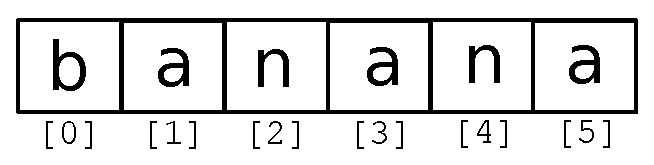
\includegraphics[height=0.50in]{figs2/string.eps}}
\afterfig

\index{index!starting at zero}
\index{zero, index starting at}

You can use any expression, including variables and operators, as an
index, but the value of the index has to be an integer.  Otherwise you
get:

\index{index}
\index{exception!TypeError}
\index{TypeError}

\beforeverb
\begin{verbatim}
>>> letter = fruit[1.5]
TypeError: string indices must be integers
\end{verbatim}
\afterverb
%

\section{Getting the length of a string using {\tt len}}

\index{len function}
\index{function!len}

{\tt len} is a built-in function that returns the number of characters
in a string:

\beforeverb
\begin{verbatim}
>>> fruit = 'banana'
>>> len(fruit)
6
\end{verbatim}
\afterverb
%
To get the last letter of a string, you might be tempted to try something
like this:

\index{exception!IndexError}
\index{IndexError}

\beforeverb
\begin{verbatim}
>>> length = len(fruit)
>>> last = fruit[length]
IndexError: string index out of range
\end{verbatim}
\afterverb
%
The reason for the {\tt IndexError} is that there is no letter in {\tt
'banana'} with the index 6.  Since we started counting at zero, the
six letters are numbered 0 to 5.  To get the last character, you have
to subtract 1 from {\tt length}:

\beforeverb
\begin{verbatim}
>>> last = fruit[length-1]
>>> print last
a
\end{verbatim}
\afterverb
%
Alternatively, you can use negative indices, which count backward from
the end of the string.  The expression {\tt fruit[-1]} yields the last
letter, {\tt fruit[-2]} yields the second to last, and so on.

\index{index!negative}
\index{negative index}


\section{Traversal through a string with a {\tt for} loop}
\label{for}

\index{traversal}
\index{loop!traversal}
\index{for loop}
\index{loop!for}
\index{statement!for}
\index{traversal}

A lot of computations involve processing a string one character at a
time.  Often they start at the beginning, select each character in
turn, do something to it, and continue until the end.  This pattern of
processing is called a {\bf traversal}.  One way to write a traversal
is with a {\tt while} loop:

\beforeverb
\begin{verbatim}
index = 0
while index < len(fruit):
    letter = fruit[index]
    print letter
    index = index + 1
\end{verbatim}
\afterverb
%
This loop traverses the string and displays each letter on a line by
itself.  The loop condition is {\tt index < len(fruit)}, so
when {\tt index} is equal to the length of the string, the
condition is false, and the body of the loop is not executed.  The
last character accessed is the one with the index {\tt len(fruit)-1},
which is the last character in the string.

\begin{ex}
Write a {\tt while} loop that starts at the last character in the string
and works its way backwards to the first character in the string, 
printing each letter on a separate line, except backwards.
\end{ex}

Another way to write a traversal is with a {\tt for} loop:

\beforeverb
\begin{verbatim}
for char in fruit:
    print char
\end{verbatim}
\afterverb
%
Each time through the loop, the next character in the string is assigned
to the variable {\tt char}.  The loop continues until no characters are
left.

\index{concatenation}
\index{abecedarian}
\index{McCloskey, Robert}

The following example shows how to use concatenation (string addition)
and a {\tt for} loop to generate an abecedarian series (that is, in
alphabetical order).  In Robert McCloskey's book \emph{Make
Way for Ducklings}, the names of the ducklings are Jack, Kack, Lack,
Mack, Nack, Ouack, Pack, and Quack.  This loop outputs these names in
order:

\beforeverb
\begin{verbatim}
prefixes = 'JKLMNOPQ'
suffix = 'ack'

for letter in prefixes:
    print letter + suffix
\end{verbatim}
\afterverb
%
The output is:

\beforeverb
\begin{verbatim}
Jack
Kack
Lack
Mack
Nack
Oack
Pack
Qack
\end{verbatim}
\afterverb
%
Of course, that's not quite right because ``Ouack'' and
``Quack'' are misspelled.


\section{String slices}
\label{slice}

\index{slice operator}
\index{operator!slice}
\index{index!slice}
\index{string!slice}
\index{slice!string}

A segment of a string is called a {\bf slice}.  Selecting a slice is
similar to selecting a character:

\beforeverb
\begin{verbatim}
>>> s = 'Monty Python'
>>> print s[0:5]
Monty
>>> print s[6:13]
Python
\end{verbatim}
\afterverb
%
The operator {\tt [n:m]} returns the part of the string from the 
``n-eth'' character to the ``m-eth'' character, including the first but
excluding the last.  This behavior is counterintuitive, but it might
help to imagine the indices pointing \emph{between} the
characters, as in the following diagram:

\beforefig
\centerline{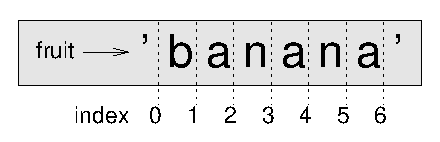
\includegraphics{figs/banana.eps}}
\afterfig

If you omit the first index (before the colon), the slice starts at
the beginning of the string.  If you omit the second index, the slice
goes to the end of the string:

\beforeverb
\begin{verbatim}
>>> fruit = 'banana'
>>> fruit[:3]
'ban'
>>> fruit[3:]
'ana'
\end{verbatim}
\afterverb
%
If the first index is greater than or equal to the second the result
is an {\bf empty string}, represented by two quotation marks:

\index{quotation mark}

\beforeverb
\begin{verbatim}
>>> fruit = 'banana'
>>> fruit[3:3]
''
\end{verbatim}
\afterverb
%
An empty string contains no characters and has length 0, but other
than that, it is the same as any other string.

\begin{ex}
Given that {\tt fruit} is a string, what does
{\tt fruit[:]} mean?

\index{copy!slice}
\index{slice!copy}


\end{ex}


\section{Strings are immutable}
\index{mutability}
\index{immutability}
\index{string!immutable}

It is tempting to use the {\tt []} operator on the left side of an
assignment, with the intention of changing a character in a string.
For example:

\index{TypeError}
\index{exception!TypeError}

\beforeverb
\begin{verbatim}
>>> greeting = 'Hello, world!'
>>> greeting[0] = 'J'
TypeError: object does not support item assignment
\end{verbatim}
\afterverb
%
The ``object'' in this case is the string and the ``item'' is
the character you tried to assign.  For now, an {\bf object} is
the same thing as a value, but we will refine that definition
later.  An {\bf item} is one of the values in a sequence.

\index{object}
\index{item assignment}
\index{assignment!item}
\index{immutability}

The reason for the error is that
strings are {\bf immutable}, which means you can't change an
existing string.  The best you can do is create a new string
that is a variation on the original:

\beforeverb
\begin{verbatim}
>>> greeting = 'Hello, world!'
>>> new_greeting = 'J' + greeting[1:]
>>> print new_greeting
Jello, world!
\end{verbatim}
\afterverb
%
This example concatenates a new first letter onto
a slice of {\tt greeting}.  It has no effect on
the original string.

\index{concatenation}

\section{Looping and counting}
\label{counter}

\index{counter}
\index{counting and looping}
\index{looping and counting}
\index{looping!with strings}

The following program counts the number of times the letter {\tt a}
appears in a string:

\beforeverb
\begin{verbatim}
word = 'banana'
count = 0
for letter in word:
    if letter == 'a':
        count = count + 1
print count
\end{verbatim}
\afterverb
%
This program demonstrates another pattern of computation called a {\bf
counter}.  The variable {\tt count} is initialized to 0 and then
incremented each time an {\tt a} is found.
When the loop exits, {\tt count}
contains the result---the total number of {\tt a}'s.

\begin{ex}
\index{encapsulation}

Encapsulate this code in a function named {\tt
count}, and generalize it so that it accepts the string and the
letter as arguments.
\end{ex}

\section{The {\tt in} operator}
\label{inboth}

\index{in operator}
\index{operator!in}
\index{boolean operator}
\index{operator!boolean}

The word {\tt in} is a boolean operator that takes two strings and
returns {\tt True} if the first appears as a substring in the second:

\beforeverb
\begin{verbatim}
>>> 'a' in 'banana'
True
>>> 'seed' in 'banana'
False
\end{verbatim}
\afterverb
%

\section{String comparison}

\index{string!comparison}
\index{comparison!string}

The comparison operators work on strings.  To see if two strings are equal:

\beforeverb
\begin{verbatim}
if word == 'banana':
    print  'All right, bananas.'
\end{verbatim}
\afterverb
%
Other comparison operations are useful for putting words in alphabetical
order:

\beforeverb
\begin{verbatim}
if word < 'banana':
    print 'Your word,' + word + ', comes before banana.'
elif word > 'banana':
    print 'Your word,' + word + ', comes after banana.'
else:
    print 'All right, bananas.'
\end{verbatim}
\afterverb
%
Python does not handle uppercase and lowercase letters the same way
that people do.  All the uppercase letters come before all the
lowercase letters, so:

\beforeverb
\begin{verbatim}
Your word, Pineapple, comes before banana.
\end{verbatim}
\afterverb
%
A common way to address this problem is to convert strings to a
standard format, such as all lowercase, before performing the
comparison.  Keep that in mind in case you have to defend yourself
against a man armed with a Pineapple.


\section{{\tt string} methods}

Strings are an example of Python {\bf objects}.  An object contains
both data (the actual string itself) as well as {\bf methods} which
are effectively functions which are built into the object and 
available to any {\bf instance} of the object.

Python has a function called {\tt dir} that lists the methods available
for an object.  The {\tt type} function shows the type of an object 
and the {\tt dir} function shows the available methods.
\beforeverb
\begin{verbatim}
>>> stuff = 'Hello world'
>>> type(stuff)
<type 'str'>
>>> dir(stuff)
['capitalize', 'center', 'count', 'decode', 'encode', 
'endswith', 'expandtabs', 'find', 'format', 'index', 
'isalnum', 'isalpha', 'isdigit', 'islower', 'isspace', 
'istitle', 'isupper', 'join', 'ljust', 'lower', 'lstrip', 
'partition', 'replace', 'rfind', 'rindex', 'rjust', 
'rpartition', 'rsplit', 'rstrip', 'split', 'splitlines', 
'startswith', 'strip', 'swapcase', 'title', 'translate', 
'upper', 'zfill']
>>> help(str.capitalize)
Help on method_descriptor:

capitalize(...)
    S.capitalize() -> string
    
    Return a copy of the string S with only its first character
    capitalized.
>>>
\end{verbatim}
\afterverb
%

While the {\tt dir} function lists the methods, and you 
can use {\tt help} to get some simple documentation on a method, 
a better source of documentation for string methods would be
\url{docs.python.org/library/string.html}.

Calling a {\bf method} is similar to calling a function---it 
takes arguments and
returns a value---but the syntax is different.  We call a method
by appending the method name to the variable name using the period 
as a delimiter.

For example, the
method {\tt upper} takes a string and returns a new string with
all uppercase letters:

\index{method}
\index{string!method}

Instead of the function syntax {\tt upper(word)}, it uses
the method syntax {\tt word.upper()}.

\index{dot notation}

\beforeverb
\begin{verbatim}
>>> word = 'banana'
>>> new_word = word.upper()
>>> print new_word
BANANA
\end{verbatim}
\afterverb
%
This form of dot notation specifies the name of the method, {\tt
upper}, and the name of the string to apply the method to, {\tt
word}.  The empty parentheses indicate that this method takes no
argument.

\index{parentheses!empty}

A method call is called an {\bf invocation}; in this case, we would
say that we are invoking {\tt upper} on the {\tt word}.

\index{invocation}

As it turns out, there is a string method named {\tt find} that
is remarkably similar to the function we wrote:

\beforeverb
\begin{verbatim}
>>> word = 'banana'
>>> index = word.find('a')
>>> print index
1
\end{verbatim}
\afterverb
%
In this example, we invoke {\tt find} on {\tt word} and pass
the letter we are looking for as a parameter.

Actually, the {\tt find} method is more general than our function;
it can find substrings, not just characters:

\beforeverb
\begin{verbatim}
>>> word.find('na')
2
\end{verbatim}
\afterverb
%
It can take as a second argument the index where it should start:

\index{optional argument}
\index{argument!optional}

\beforeverb
\begin{verbatim}
>>> word.find('na', 3)
4
\end{verbatim}
\afterverb
%
One common task is to remove white space (spaces, tabs, or newlines) from
the beginning and end of a string using the {\tt strip} method:

\beforeverb
\begin{verbatim}
>>> line = '  Here we go  '
>>> line.strip()
'Here we go'
\end{verbatim}
\afterverb
%
Some methods such as {\bf startswith} return boolean values.

\beforeverb
\begin{verbatim}
>>> line = 'Please have a nice day'
>>> line.startswith('Please')
True
>>> line.startswith('p')
False
\end{verbatim}
\afterverb
%
You will note that {\tt startswith} requires case to match so sometimes
we take a line and map it all to lowercase before we do any checking
using the {\tt lower} method.

\beforeverb
\begin{verbatim}
>>> line = 'Please have a nice day'
>>> line.startswith('p')
False
>>> line.lower()
'please have a nice day'
>>> line.lower().startswith('p')
True
\end{verbatim}
\afterverb
%
In the last example, the method {\tt lower} is called
and then we use {\tt startswith}
to check to see if the resulting lowercase string
starts with the letter ``p''.  As long as we are careful
with the order, we can make multiple method calls in a
single expression.

\begin{ex}
\index{count method}
\index{method!count}

There is a string method called {\tt count} that is similar
to the function in the previous exercise.  Read the documentation
of this method at
\url{docs.python.org/library/string.html}
and write an invocation that counts the number of times the 
letter a  occurs
in \verb"'banana'".
\end{ex}

\section{Parsing strings}

Often, we want to look into a string and find a substring.  For example
if we were presented a series of lines formatted as follows:

{\tt
From stephen.marquard@{\bf uct.ac.za} Sat Jan  5 09:14:16 2008
}

And we wanted to pull out only the second half of the address (i.e.
{\tt uct.ac.za}) from each line.  We can do this by using the {\tt find}
method and string slicing.   

First, we will find the position of the at-sign in the string.  Then we will
find the position of the first space \emph{after} the at-sign.  And then we
will use string slicing to extract the portion of the string which we 
are looking for.

\beforeverb
\begin{verbatim}
>>> data = 'From stephen.marquard@uct.ac.za Sat Jan  5 09:14:16 2008'
>>> atpos = data.find('@')
>>> print atpos
21
>>> sppos = data.find(' ',atpos)
>>> print sppos
31
>>> host = data[atpos+1:sppos]
>>> print host
uct.ac.za
>>> 
\end{verbatim}
\afterverb
%
We use a version of the {\tt find} method which allows us to specify
a position in the string where we want {\tt find} to start looking.
When we slice, we extract the characters 
from ``one beyond the at-sign through up to \emph{but not including} the 
space character''.  

The documentation for the {\tt find} method is available at
\url{docs.python.org/library/string.html}.

\section{Format operator}

\index{format operator}
\index{operator!format}

The {\bf format operator}, {\tt \%}
allows us to construct strings, replacing parts of the strings
with the data stored in variables.
When applied to integers, {\tt \%} is the modulus operator.  But
when the first operand is a string, {\tt \%} is the format operator.

\index{format string}

The first operand is the {\bf format string}, which contains
one or more {\bf format sequences}, which
specify how
the second operand is formatted.  The result is a string.

\index{format sequence}

For example, the format sequence \verb"'%d'" means that
the second operand should be formatted as an
integer ({\tt d} stands for ``decimal''):

\beforeverb
\begin{verbatim}
>>> camels = 42
>>> '%d' % camels
'42'
\end{verbatim}
\afterverb
%
The result is the string \verb"'42'", which is not to be confused
with the integer value {\tt 42}.

A format sequence can appear anywhere in the string,
so you can embed a value in a sentence:

\beforeverb
\begin{verbatim}
>>> camels = 42
>>> 'I have spotted %d camels.' % camels
'I have spotted 42 camels.'
\end{verbatim}
\afterverb
%
If there is more than one format sequence in the string,
the second argument has to be a tuple.  Each format sequence is
matched with an element of the tuple, in order.

The following example uses \verb"'%d'" to format an integer,
\verb"'%g'" to format
a floating-point number (don't ask why), and \verb"'%s'" to format
a string:

\beforeverb
\begin{verbatim}
>>> 'In %d years I have spotted %g %s.' % (3, 0.1, 'camels')
'In 3 years I have spotted 0.1 camels.'
\end{verbatim}
\afterverb
%
The number of elements in the tuple has to match the number
of format sequences in the string.  Also, the types of the
elements have to match the format sequences:

\index{exception!TypeError}
\index{TypeError}

\beforeverb
\begin{verbatim}
>>> '%d %d %d' % (1, 2)
TypeError: not enough arguments for format string
>>> '%d' % 'dollars'
TypeError: illegal argument type for built-in operation
\end{verbatim}
\afterverb
%
In the first example, there aren't enough elements; in the
second, the element is the wrong type.

The format operator is powerful, but it can be difficult to use.  You
can read more about it at
\url{docs.python.org/lib/typesseq-strings.html}.

% You can specify the number of digits as part of the format sequence.
% For example, the sequence \verb"'%8.2f'"
% formats a floating-point number to be 8 characters long, with
% 2 digits after the decimal point:

% \beforeverb
% \begin{verbatim}
% >>> '%8.2f' % 3.14159
% '    3.14'
% \end{verbatim}
% \afterverb
% %
% The result takes up eight spaces with two
% digits after the decimal point.  


\section{Debugging}
\index{debugging}

A skill that you should cultivate as you program is always
asking yourself, ``What could go wrong here?'' or alternatively,
``What crazy thing might our user do to crash our (seemingly) 
perfect program?''.

For example, look at the program which we used to demonstrate
the {\tt while} loop in the chapter on iteration:

\beforeverb
\begin{verbatim}
while True:
    line = raw_input('> ')
    if line[0] == '#' :
        continue
    if line == 'done':
        break
    print line

print 'Done!'
\end{verbatim}
\afterverb
%
Look what happens when the user enters an empty line of input:

\beforeverb
\begin{verbatim}
> hello there
hello there
> # don't print this
> print this!
print this!
> 
Traceback (most recent call last):
  File "copytildone.py", line 3, in <module>
    if line[0] == '#' :
\end{verbatim}
\afterverb
%
The code works fine until it is presented an empty line.  Then
there is no zeroth character so we get a traceback.  There are two
solutions to this to make line three ``safe'' even if the line is 
empty.

One possibility is to simply use the {\tt startswith} method
which returns {\tt False} if the string is empty.

\beforeverb
\begin{verbatim}
    if line.startswith('#') :
\end{verbatim}
\afterverb
%
\index{guardian pattern}
\index{pattern!guardian}
Another way to safely write the {\tt if} statement using the {\bf guardian}
pattern and make sure the second logical expression is evaluated 
only where there is at least one character in the string.:

\beforeverb
\begin{verbatim}
    if len(line) > 0 and line[0] == '#' :
\end{verbatim}
\afterverb
%

\section{Glossary}

\begin{description}

\item[counter:] A variable used to count something, usually initialized
to zero and then incremented.
\index{counter}

\item[empty string:] A string with no characters and length 0, represented
by two quotation marks.
\index{empty string}

\item[format operator:] An operator, {\tt \%}, that takes a format
string and a tuple and generates a string that includes
the elements of the tuple formatted as specified by the format string.
\index{format operator}
\index{operator!format}

\item[format sequence:] A sequence of characters in a format string,
like {\tt \%d}, that specifies how a value should be formatted.
\index{format sequence}

\item[format string:] A string, used with the format operator, that
contains format sequences.
\index{format string}

\item[flag:] A boolean variable used to indicate whether a condition
is true.
\index{flag}

\item[invocation:] A statement that calls a method.
\index{invocation}

\item[immutable:] The property of a sequence whose items cannot
be assigned.
\index{immutability}

\item[index:] An integer value used to select an item in
a sequence, such as a character in a string.
\index{index}

\item[item:] One of the values in a sequence.
\index{item}

\item[method:] A function that is associated with an object and called
using dot notation.
\index{method}

\item[object:] Something a variable can refer to.  For now,
you can use ``object'' and ``value'' interchangeably.
\index{object}

\item[search:] A pattern of traversal that stops
when it finds what it is looking for.
\index{search pattern}
\index{pattern!search}

\item[sequence:] An ordered set; that is, a set of
values where each value is identified by an integer index.
\index{sequence}

\item[slice:] A part of a string specified by a range of indices.
\index{slice}

\item[traverse:] To iterate through the items in a sequence,
performing a similar operation on each.
\index{traversal}

\end{description}


\section{Exercises}

\begin{ex}
Take the following Python code that stores a string:`

{\tt
str = 'X-DSPAM-Confidence: {\bf 0.8475}'
}

Use {\tt find} and string slicing to extract the portion
of the string after the colon character and then use the 
{\tt float} function to convert the extracted string 
into a floating point number.

\end{ex}


\begin{ex}
\index{string method}
\index{method!string}

Read the documentation of the string methods at
\url{docs.python.org/lib/string-methods.html}.  You
might want to experiment with some of them to make sure
you understand how they work.  {\tt strip} and
{\tt replace} are particularly useful.

The documentation uses a syntax that might be confusing.
For example, in \verb"find(sub[, start[, end]])", the brackets
indicate optional arguments.  So {\tt sub} is required, but
{\tt start} is optional, and if you include {\tt start},
then {\tt end} is optional.
\end{ex}

\chapter{Files}

\index{file}
\index{type!file}


\section{Persistence}

\index{persistence}
\index{secondary memory}

So far, we have learned how to write programs and communicate 
our intentions to the {\bf Central Processing Unit} using conditional
execution, functions, and iterations.  We have learned how to 
create and use data structures in the {\bf Main Memory}.  The CPU 
and memory are where our software works and runs.  It is where 
all of the ``thinking'' happens.  

But if you recall from our hardware architecture discussions,
once the power is turned off, anything stored in either
the CPU or main memory is erased.  So up to now, our
programs have just been transient fun exercises to learn Python.

\beforefig
\centerline{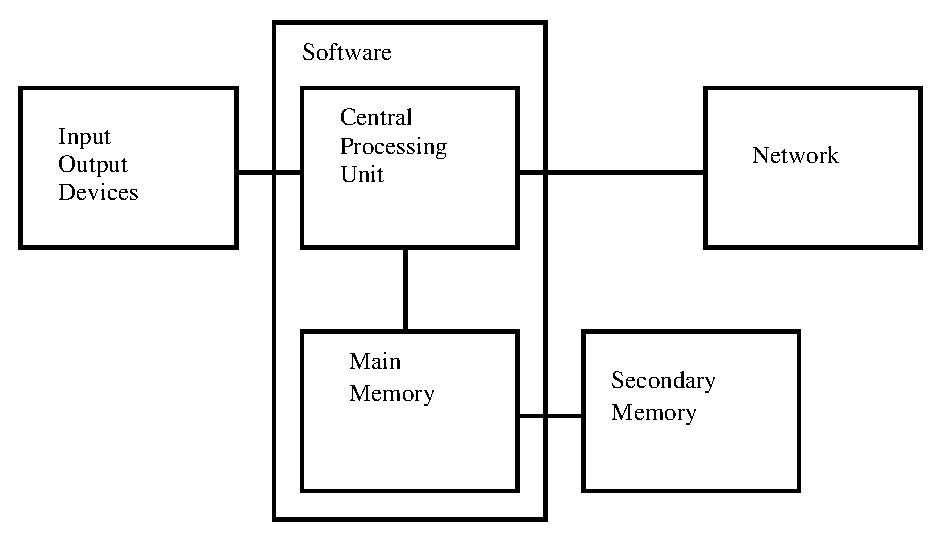
\includegraphics[height=2.50in]{figs2/arch3.eps}}
\afterfig

In this chapter, we start to work with {\bf Secondary Memory} 
(or files).
Secondary memory is not erased even when the power is turned off.  
Or in the case of a USB flash drive, the
data can we write from our programs can be removed from the 
system and transported to another system.

We will primarily focus on reading and writing text files such as 
those we create in a text editor.  Later we will see how to work
with database files which are binary files, specifically designed to be read
and written through database software.

\section{Opening files}
\index{file!open}
\index{open function}
\index{function!open}

When we want to read or write a file (say on your hard drive), we first
must {\bf open} the file.  Opening the file communicates with your operating
system which knows where the data for each file is stored.  When you open
a file, you are asking the operating system to find the file by name
and make sure the file exists.  In this example, we open the file 
{\tt mbox.txt} which should be stored in the same folder that you
are in when you 
start Python.
You can download this file from 
\url{www.py4inf.com/code/mbox.txt}

\beforeverb
\begin{verbatim}
>>> fhand = open('mbox.txt')
>>> print fhand
<open file 'mbox.txt', mode 'r' at 0x1005088b0>
\end{verbatim}
\afterverb
%
\index{file handle}
If the {\tt open} is successful, the operating system returns us a 
{\bf file handle}.  The file handle is not the actual data contained
in the file, but instead it is a ``handle'' that we can use to 
read the data.   You are given a handle if the requested file
exists and you have the proper permissions to read the file.

\beforefig
\centerline{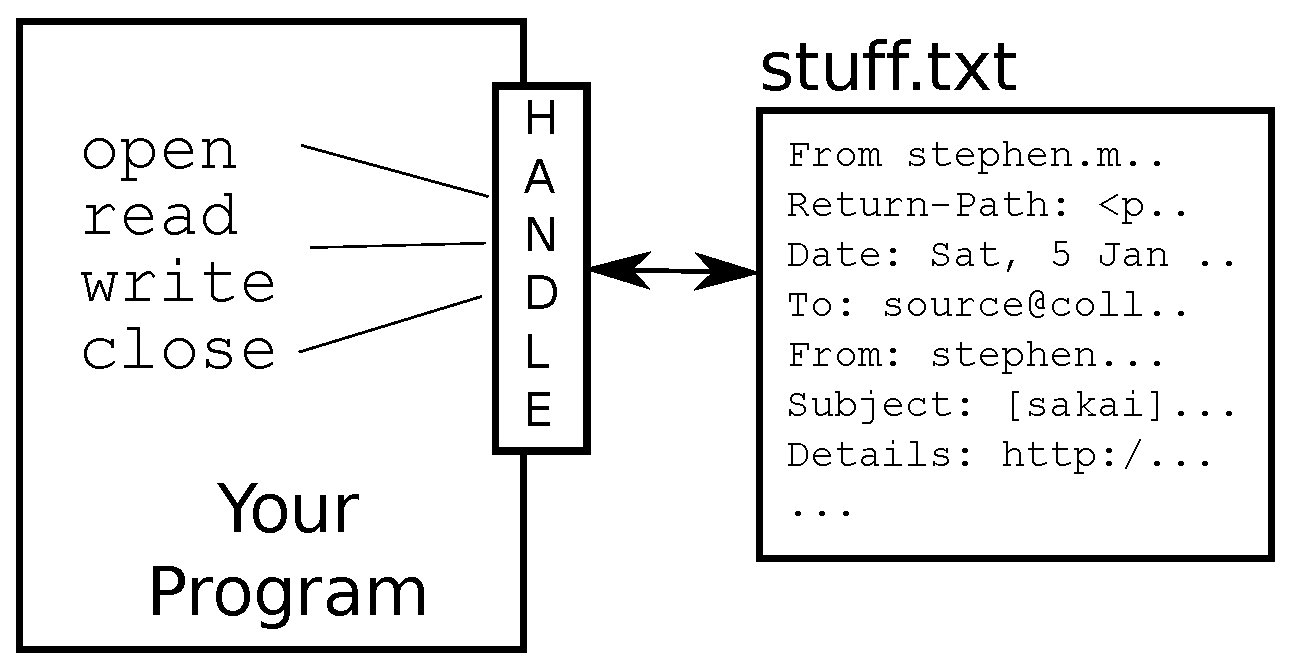
\includegraphics[height=1.75in]{figs2/handle.eps}}
\afterfig

If the file does not exist, {\tt open} will fail with a traceback and you 
will not get a handle to access the contents of the file:

\beforeverb
\begin{verbatim}
>>> fhand = open('stuff.txt')
Traceback (most recent call last):
  File "<stdin>", line 1, in <module>
IOError: [Errno 2] No such file or directory: 'stuff.txt'
\end{verbatim}
\afterverb
%
Later we will use {\tt try} and {\tt except} to deal more gracefully
with the situation where we attempt to open a file that does 
not exist.

\section{Text files and lines}

A text file can be thought of as a sequence of lines, much like a Python
string can be thought of as a sequence of characters.  For example, this
is a sample of a text file which records mail activity from various
individuals in an open source project development team:

{\tt
From stephen.marquard@uct.ac.za Sat Jan  5 09:14:16 2008\\
Return-Path: <postmaster@collab.sakaiproject.org>\\
Date: Sat, 5 Jan 2008 09:12:18 -0500\\
To: source@collab.sakaiproject.org\\
From: stephen.marquard@uct.ac.za\\
Subject: [sakai] svn commit: r39772 - content/branches/\\
Details: http://source.sakaiproject.org/viewsvn/?view=rev\&rev=39772\\
...
}

The entire file of mail interactions is available from 
\url{www.py4inf.com/code/mbox.txt} 
and a shortened version of the file is available from
\url{www.py4inf.com/code/mbox-short.txt}.
These files are in a standard format for a file containing 
multiple mail messages. The lines which start with 
``From '' separate the messages and the lines which start 
with ``From:'' are part of the messages. 
For more information, see 
\url{en.wikipedia.org/wiki/Mbox}. 

To break the file into lines, there is a special character that 
represents the ``end of the line'' called the {\bf newline} character.

\index{newline}
In Python, we represent the {\bf newline} character as a backslash-n in 
string constants.  Even though this looks like two characters, it
is actually a single character.  When we look at the variable by entering
``stuff'' in the interpreter, it shows us the \verb"\n" in the string, 
but when we use {\tt print} to show the string, we see the string broken
into two lines by the newline character.

\beforeverb
\begin{verbatim}
>>> stuff = 'Hello\nWorld!'
>>> stuff
'Hello\nWorld!'
>>> print stuff
Hello
World!
>>> stuff = 'X\nY'
>>> print stuff
X
Y
>>> len(stuff)
3
\end{verbatim}
\afterverb
%

You can also see that the length of the string \verb"'X\nY'" is \emph{three}
characters because the newline character is a single character.

So when we look at the lines in a file, we need to \emph{imagine}
that there is a special invisible character at the end of each line
that marks the end of the line called the newline.  

{\tt
From stephen.marquard@uct.ac.za Sat Jan  5 09:14:16 2008\verb"\n"\\
Return-Path: <postmaster@collab.sakaiproject.org>\verb"\n"\\
Date: Sat, 5 Jan 2008 09:12:18 -0500\verb"\n"\\
To: source@collab.sakaiproject.org\verb"\n"\\
From: stephen.marquard@uct.ac.za\verb"\n"\\
Subject: [sakai] svn commit: r39772 - content/branches/\verb"\n"\\
Details: http://source.sakaiproject.org/viewsvn/?view=rev\&rev=39772\verb"\n"\\
...
}

So the newline character separates the characters 
in the file into lines.

\section{Reading files}

\index{file!reading}
\index{counter}
While the {\bf file handle} does not contain the data for the file,
it is quite easy to construct a {\tt for} loop to read through 
and count each of the lines in a file:

\beforeverb
\begin{verbatim}
fhand = open('mbox.txt')
count = 0
for line in fhand:
    count = count + 1
print 'Line Count:', count

python open.py 
Line Count: 132045
\end{verbatim}
\afterverb
%
We can use the file handle as the sequence in our {\tt for} loop.  
Our {\tt for} loop simply counts the number of lines in the 
file and prints them out.  The rough translation of the {\tt for}
loop into English is, ``for each line in the file represented by the file
handle, add one to the {\tt count} variable.''

The reason that the {\tt open} function does not read the entire file
is that the file might be quite large with many gigabytes of data.
The {\tt open} statement takes the same amount of time regardless of the
size of the file.  The {\tt for} loop actually causes the data to be 
read from the file.

When the file is read using a {\tt for} loop in this manner, Python
takes care of splitting the data in the file into separate lines using
the newline character.  Python reads each line through 
the newline and includes
the newline as the last character in the {\tt line} variable for each 
iteration of the {\tt for} loop.

Because the for loop reads the data one line at a time, it can efficiently
read and count the lines in very large files without running 
out of main memory to store the data.  The above program can 
count the lines in any size file using very little memory since 
each line is read, counted, and then discarded.

If you know the file is relatively small compared to the size of 
your main memory, you can read the whole file into one string
using the {\tt read} method on the file handle.

\beforeverb
\begin{verbatim}
>>> fhand = open('mbox-short.txt')
>>> inp = fhand.read()
>>> print len(inp)
94626
>>> print inp[:20]
From stephen.marquar
\end{verbatim}
\afterverb
%
In this example, the entire contents (all 94,626 characters) 
of the file {\tt mbox-short.txt} are read directly into the 
variable {\tt inp}.  We use string slicing to print out the first
20 characters of the string data stored in {\tt inp}.

When the file is read in this manner, all the characters including 
all of the lines and newline characters are one big string 
in the variable {\bf inp}.  
Remember that this form of the {\tt open} function should only be used
if the file data will fit comfortably in the main memory 
of your computer.

If the file is too large to fit in main memory, you should write
your program to read the file in chunks using a {\tt for} or {\tt while}
loop.

\section{Searching through a file}

When you are searching through data in a file, it
is a very common pattern to read through a file, ignoring most
of the lines and only processing lines which meet a particular criteria.
We can combine the pattern for reading a file with string {\bf methods}
to build simple search mechanisms.

\index{filter pattern}
\index{pattern!filter}
For example, if we wanted to read a file and only print out lines
which started with the prefix ``From:'', we could use the 
string method {\bf startswith} to select only those lines with
the desired prefix:

\beforeverb
\begin{verbatim}
fhand = open('mbox-short.txt')
for line in fhand:
    if line.startswith('From:') :
        print line
\end{verbatim}
\afterverb
%
When this program runs, we get the following output:

\beforeverb
\begin{verbatim}
From: stephen.marquard@uct.ac.za

From: louis@media.berkeley.edu

From: zqian@umich.edu

From: rjlowe@iupui.edu
...
\end{verbatim}
\afterverb
%
The output looks great since the only lines we are seeing are those 
which start with ``From:'', but why are we seeing the extra blank
lines?  This is due to that invisible {\bf newline} character.
Each of the lines ends with a newline, so the {\tt print} 
statement prints the string in the variable {\bf line} which includes
a newline and then {\tt print} adds \emph{another} newline, resulting
in the double spacing effect we see.

We could use line slicing to print all but the last character, but 
a simpler approach is to use the {\bf rstrip} method which strips
whitespace from the right side of a string as follows:

\beforeverb
\begin{verbatim}
fhand = open('mbox-short.txt')
for line in fhand:
    line = line.rstrip()
    if line.startswith('From:') :
        print line
\end{verbatim}
\afterverb
%
When this program runs, we get the following output:

\beforeverb
\begin{verbatim}
From: stephen.marquard@uct.ac.za
From: louis@media.berkeley.edu
From: zqian@umich.edu
From: rjlowe@iupui.edu
From: zqian@umich.edu
From: rjlowe@iupui.edu
From: cwen@iupui.edu
...
\end{verbatim}
\afterverb
%
As your file processing programs get more complicated, you may want 
to structure your search loops using {\tt continue}.  The basic idea 
of the search loop is that you are looking for ``interesting'' lines
and effectively skipping ``uninteresting'' lines.  And then when we
find an interesting line, we do something with that line.

We can structure the loop to follow the
pattern of skipping uninteresting lines as follows:

\beforeverb
\begin{verbatim}
fhand = open('mbox-short.txt')
for line in fhand:
    line = line.rstrip()
    # Skip 'uninteresting lines'
    if not line.startswith('From:') :
        continue
    # Process our 'interesting' line
    print line
\end{verbatim}
\afterverb
%
The output of the program is the same.  In English, the 
uninteresting lines are those which do not start 
with ``From:'', which we skip using {\tt continue}.
For the ``interesting'' lines (i.e. those that start with ``From:'')
we perform the processing on those lines.

We can use the {\tt find} string method to simulate a text editor
search which finds lines where the search string is anywhere in the line.  
Since {\tt find} looks for an occurrence of a string within another
string and either returns the position of the string or -1 if the string
was not found, we can write the following loop to show lines which
contain the string ``@uct.ac.za'' (i.e. they come from the University 
of Cape Town in South Africa):

\beforeverb
\begin{verbatim}
fhand = open('mbox-short.txt')
for line in fhand:
    line = line.rstrip()
    if line.find('@uct.ac.za') == -1 : 
        continue
    print line
\end{verbatim}
\afterverb
%
Which produces the following output:

\beforeverb
\begin{verbatim}
From stephen.marquard@uct.ac.za Sat Jan  5 09:14:16 2008
X-Authentication-Warning: set sender to stephen.marquard@uct.ac.za using -f
From: stephen.marquard@uct.ac.za
Author: stephen.marquard@uct.ac.za
From david.horwitz@uct.ac.za Fri Jan  4 07:02:32 2008
X-Authentication-Warning: set sender to david.horwitz@uct.ac.za using -f
From: david.horwitz@uct.ac.za
Author: david.horwitz@uct.ac.za
...
\end{verbatim}
\afterverb
%

\section{Letting the user choose the file name}

We really do not want to have to edit our Python code
every time we want to process a different file.  It would 
be more usable to ask the user to enter the file name string 
each time the program runs so they can use our 
program on different files without changing the Python code.

This is quite simple to do by reading the file name from
the user using \verb"raw_input" as follows:

\beforeverb
\begin{verbatim}
fname = raw_input('Enter the file name: ')
fhand = open(fname)
count = 0
for line in fhand:
    if line.startswith('Subject:') :
        count = count + 1
print 'There were', count, 'subject lines in', fname
\end{verbatim}
\afterverb
%
We read the file name from the user and place it in a variable
named {\tt fname} and open that file.  Now we can run the program 
repeatedly on different files.

\beforeverb
\begin{verbatim}
python search6.py 
Enter the file name: mbox.txt
There were 1797 subject lines in mbox.txt

python search6.py 
Enter the file name: mbox-short.txt
There were 27 subject lines in mbox-short.txt
\end{verbatim}
\afterverb
%
Before peeking at the next section, take a look at the above program
and ask yourself, ``What could go possibly wrong here?'' or ``What might our
friendly user do that would cause our nice little program to 
ungracefully exit with a traceback, making us look not-so-cool 
in the eyes of our users?''.

\section{Using {\tt try, except,} and {\tt open}}

I told you not to peek.  This is your last chance.

What if our user types something that is not a file name?
\beforeverb
\begin{verbatim}
python search6.py 
Enter the file name: missing.txt
Traceback (most recent call last):
  File "search6.py", line 2, in <module>
    fhand = open(fname)
IOError: [Errno 2] No such file or directory: 'missing.txt'

python search6.py 
Enter the file name: na na boo boo
Traceback (most recent call last):
  File "search6.py", line 2, in <module>
    fhand = open(fname)
IOError: [Errno 2] No such file or directory: 'na na boo boo'
\end{verbatim}
\afterverb
%
Do not laugh, users will eventually do every possible thing they can do 
to break your programs --- either on purpose or with malicious intent.
As a matter of fact, an important part of any software development
team is a person or group called {\bf Quality Assurance} (or QA for short)
whose very job it is to do the craziest things possible in an attempt
to break the software that the programmer has created.

\index{Quality Assurance}
\index{QA}
The QA team is responsible for finding the flaws in programs before 
we have delivered the program to the end-users who may be purchasing the
software or paying our salary to write the software.  So the QA team
is the programmer's best friend.

\index{try statement}
\index{statement!try}
\index{open function}
\index{function!open}
\index{exception!IOError}
\index{IOError}
So now that we see the flaw in the program, we can elegantly fix it using
the {\tt try}/{\tt except} structure.  We need to assume that the {\tt open}
call might fail and add recovery code when the {\tt open} fails
as follows:

\beforeverb
\begin{verbatim}
fname = raw_input('Enter the file name: ')
try:
    fhand = open(fname)
except:
    print 'File cannot be opened:', fname
    exit()

count = 0
for line in fhand:
    if line.startswith('Subject:') : 
        count = count + 1
print 'There were', count, 'subject lines in', fname
\end{verbatim}
\afterverb
%
The {\tt exit} function terminates the program.  It is a function
that we call that never returns.  Now when our user (or 
QA team) types in silliness or bad file names, 
we ``catch'' them and recover gracefully:
\beforeverb
\begin{verbatim}
python search7.py
Enter the file name: mbox.txt
There were 1797 subject lines in mbox.txt

python search7.py
Enter the file name: na na boo boo
File cannot be opened: na na boo boo
\end{verbatim}
\afterverb
%
\index{Pythonic}
Protecting the {\tt open} call is a good example 
of the proper use of {\tt try}
and {\tt except} in a Python program.  We use the term
``Pythonic'' when we are doing something the ``Python
way''.  We might say that the above example is 
the Pythonic way to open a file.

Once you become more skilled in Python, you can engage
in repartee' with other Python programmers to decide
which of two equivalent solutions to a problem is 
``more Pythonic''.  The goal to be ``more Pythonic'' 
captures the notion that programming is part engineering
and part art.  We are not always interested
in just making something work, we also want
our solution to be elegant and to be appreciated as 
elegant by our peers.


\section{Writing files}

\index{file!writing}

To write a file, you have to open it with mode
\verb"'w'" as a second parameter:

\beforeverb
\begin{verbatim}
>>> fout = open('output.txt', 'w')
>>> print fout
<open file 'output.txt', mode 'w' at 0xb7eb2410>
\end{verbatim}
\afterverb
%
If the file already exists, opening it in write mode clears out
the old data and starts fresh, so be careful!
If the file doesn't exist, a new one is created.

The {\tt write} method of the file handle object 
puts data into the file.

\beforeverb
\begin{verbatim}
>>> line1 = 'This here's the wattle,\n'
>>> fout.write(line1)
\end{verbatim}
\afterverb
%
\index{newline}
Again, the file object keeps track of where it is, so if
you call {\tt write} again, it adds the new data to the end.

We must make sure to manage the ends of lines as we write
to the file by explicitly inserting the newline character
when we want to end a line.  The {\tt print} statement 
automatically appends a newline, but the {\tt write} 
method does not add the newline automatically.

\beforeverb
\begin{verbatim}
>>> line2 = 'the emblem of our land.\n'
>>> fout.write(line2)
\end{verbatim}
\afterverb
%
When you are done writing, you have to close the file
to make sure that the last bit of data is physically written
to the disk so it will not be lost if the power goes off.

\beforeverb
\begin{verbatim}
>>> fout.close()
\end{verbatim}
\afterverb
%
We could close the files which we open for read as well, 
but we can be a little sloppy if we are only opening a few
files since Python makes sure that all open files are 
closed when the program ends.  When we are writing files, 
we want to explicitly close the files so as to leave nothing
to chance.

\index{close method}
\index{method!close}


\section{Debugging}

\index{debugging}
\index{whitespace}

When you are reading and writing files, you might run into problems
with whitespace.  These errors can be hard to debug because spaces,
tabs and newlines are normally invisible:

\beforeverb
\begin{verbatim}
>>> s = '1 2\t 3\n 4'
>>> print s
1 2	 3
 4
\end{verbatim}
\afterverb

\index{repr function}
\index{function!repr}
\index{string representation}

The built-in function {\tt repr} can help.  It takes any object as an
argument and returns a string representation of the object.  For
strings, it represents whitespace
characters with backslash sequences:

\beforeverb
\begin{verbatim}
>>> print repr(s)
'1 2\t 3\n 4'
\end{verbatim}
\afterverb

This can be helpful for debugging.

One other problem you might run into is that different systems
use different characters to indicate the end of a line.  Some
systems use a newline, represented \verb"\n".  Others use
a return character, represented \verb"\r".  Some use both.
If you move files between different systems, these inconsistencies
might cause problems.

\index{end of line character}

For most systems, there are applications to convert from one
format to another.  You can find them (and read more about this
issue) at \url{wikipedia.org/wiki/Newline}.  Or, of course, you
could write one yourself.

% TBD - Doesn't Python take care of this for us????

\section{Glossary}

\begin{description}

\item[catch:] To prevent an exception from terminating
a program using the {\tt try}
and {\tt except} statements.
\index{catch}

\item[newline:] A special character used in files and strings to indicate
the end of a line.
\index{newline}

\item[Pythonic:] A technique that works elegantly in Python.
``Using try and except is the \emph{Pythonic} way to recover from 
missing files.''.
\index{Pythonic}

\item[Quality Assurance:] A person or team focused on insuring the 
overall quality of a software product.  QA is often involved 
in testing a product and identifying problems before the product 
is released.
\index{Quality Assurance}
\index{QA}

\item[text file:] A sequence of characters stored in permanent
storage like a hard drive.
\index{text file}

\end{description}


\section{Exercises}

\begin{ex}
Write a program to read through a file and print the contents 
of the file (line by line) all in upper case.  Executing the program 
will look as follows:

\beforeverb
\begin{verbatim}
python shout.py
Enter a file name: mbox-short.txt
FROM STEPHEN.MARQUARD@UCT.AC.ZA SAT JAN  5 09:14:16 2008
RETURN-PATH: <POSTMASTER@COLLAB.SAKAIPROJECT.ORG>
RECEIVED: FROM MURDER (MAIL.UMICH.EDU [141.211.14.90])
	 BY FRANKENSTEIN.MAIL.UMICH.EDU (CYRUS V2.3.8) WITH LMTPA;
	 SAT, 05 JAN 2008 09:14:16 -0500
\end{verbatim}
\afterverb
%
You can download the file from
\url{www.py4inf.com/code/mbox-short.txt}
\end{ex}

\begin{ex}
Write a program 
to prompt for a file name an then read through the file 
and look for lines of the form:

{\tt
X-DSPAM-Confidence: {\bf 0.8475}
}

When you encounter a line that starts with 
``X-DSPAM-Confidence:'' pull apart the line to extract the
floating point number on the line.  Count these 
lines and the compute the total of the spam confidence 
values from these lines.
When you reach the end of the file, print out the average
spam confidence.

\beforeverb
\begin{verbatim}
Enter the file name: mbox.txt
Average spam confidence: 0.894128046745

Enter the file name: mbox-short.txt
Average spam confidence: 0.750718518519
\end{verbatim}
\afterverb
%
Test your file on the {\tt mbox.txt} and {\tt mbox-short.txt} files.
\end{ex}


\begin{ex}
Sometimes when programmers get bored or want to have a bit of fun,
they add a harmless {\bf Easter Egg} to their program 
(\url{en.wikipedia.org/wiki/Easter_egg_(media)}). Modify the program
that prompts the user for the file name so that it prints a funny
message when the user types in the exact file name 'na na boo boo'. 
The program should behave normally for all other files which exist
and don't exist.  Here is a sample execution of the program:

\beforeverb
\begin{verbatim}
python egg.py 
Enter the file name: mbox.txt
There were 1797 subject lines in mbox.txt

python egg.py 
Enter the file name: missing.tyxt
File cannot be opened: missing.tyxt

python egg.py 
Enter the file name: na na boo boo
NA NA BOO BOO TO YOU - You have been punk'd!
\end{verbatim}
\afterverb
%
We are not encouraging you to put Easter Eggs in your programs -
this is just an exercise.

\end{ex}

\chapter{Lists}

\index{list}
\index{type!list}


\section{A list is a sequence}

Like a string, a {\bf list} is a sequence of values.  In a string, the
values are characters; in a list, they can be any type.  The values in
list are called {\bf elements} or sometimes {\bf items}.

\index{element}
\index{sequence}
\index{item}

There are several ways to create a new list; the simplest is to
enclose the elements in square brackets (\verb"[" and \verb"]"):

\beforeverb
\begin{verbatim}
[10, 20, 30, 40]
['crunchy frog', 'ram bladder', 'lark vomit']
\end{verbatim}
\afterverb
%
The first example is a list of four integers.  The second is a list of
three strings.  The elements of a list don't have to be the same type.
The following list contains a string, a float, an integer, and
(lo!) another list:

\beforeverb
\begin{verbatim}
['spam', 2.0, 5, [10, 20]]
\end{verbatim}
\afterverb
%
A list within another list is {\bf nested}.

\index{nested list}
\index{list!nested}

A list that contains no elements is
called an empty list; you can create one with empty
brackets, \verb"[]".

\index{empty list}
\index{list!empty}

As you might expect, you can assign list values to variables:

\beforeverb
\begin{verbatim}
>>> cheeses = ['Cheddar', 'Edam', 'Gouda']
>>> numbers = [17, 123]
>>> empty = []
>>> print cheeses, numbers, empty
['Cheddar', 'Edam', 'Gouda'] [17, 123] []
\end{verbatim}
\afterverb
%

\index{assignment}

\section{Lists are mutable}

\index{list!element}
\index{access}
\index{index}
\index{bracket operator}
\index{operator!bracket}

The syntax for accessing the elements of a list is the same as for
accessing the characters of a string---the bracket operator.  The
expression inside the brackets specifies the index.  Remember that the
indices start at 0:

\beforeverb
\begin{verbatim}
>>> print cheeses[0]
Cheddar
\end{verbatim}
\afterverb
%
Unlike strings, lists are mutable.  When the bracket operator appears
on the left side of an assignment, it identifies the element of the
list that will be assigned.

\index{mutability}

\beforeverb
\begin{verbatim}
>>> numbers = [17, 123]
>>> numbers[1] = 5
>>> print numbers
[17, 5]
\end{verbatim}
\afterverb
%
The one-eth element of {\tt numbers}, which
used to be 123, is now 5.

\index{index!starting at zero}
\index{zero, index starting at}

You can think of a list as a relationship between indices and
elements.  This relationship is called a {\bf mapping}; each index
``maps to'' one of the elements.  Here is a state diagram showing {\tt
cheeses}, {\tt numbers} and {\tt empty}:

\index{state diagram}
\index{diagram!state}
\index{mapping}

\beforefig
\centerline{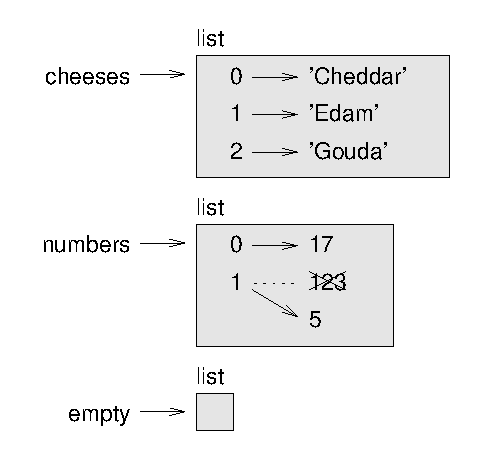
\includegraphics{figs/list_state.eps}}
\afterfig

Lists are represented by boxes with the word ``list'' outside
and the elements of the list inside.  {\tt cheeses} refers to
a list with three elements indexed 0, 1 and 2.
{\tt numbers} contains two elements; the diagram shows that the
value of the second element has been reassigned from 123 to 5.
{\tt empty} refers to a list with no elements.

\index{item assignment}
\index{assignment!item}

List indices work the same way as string indices:

\begin{itemize}

\item Any integer expression can be used as an index.

\item If you try to read or write an element that does not exist, you
get an {\tt IndexError}.

\index{exception!IndexError}
\index{IndexError}

\item If an index has a negative value, it counts backward from the
end of the list.

\end{itemize}

\index{list!index}


\index{list!membership}
\index{membership!list}
\index{in operator}
\index{operator!in}

The {\tt in} operator also works on lists.

\beforeverb
\begin{verbatim}
>>> cheeses = ['Cheddar', 'Edam', 'Gouda']
>>> 'Edam' in cheeses
True
>>> 'Brie' in cheeses
False
\end{verbatim}
\afterverb


\section{Traversing a list}
\index{list!traversal}
\index{traversal!list}
\index{for loop}
\index{loop!for}
\index{statement!for}

The most common way to traverse the elements of a list is
with a {\tt for} loop.  The syntax is the same as for strings:

\beforeverb
\begin{verbatim}
for cheese in cheeses:
    print cheese
\end{verbatim}
\afterverb
%
This works well if you only need to read the elements of the
list.  But if you want to write or update the elements, you
need the indices.  A common way to do that is to combine
the functions {\tt range} and {\tt len}:

\index{looping!with indices}
\index{index!looping with}

\beforeverb
\begin{verbatim}
for i in range(len(numbers)):
    numbers[i] = numbers[i] * 2
\end{verbatim}
\afterverb
%
This loop traverses the list and updates each element.  {\tt len}
returns the number of elements in the list.  {\tt range} returns
a list of indices from 0 to $n-1$, where $n$ is the length of
the list.  Each time through the loop {\tt i} gets the index
of the next element.  The assignment statement in the body uses
{\tt i} to read the old value of the element and to assign the
new value.

\index{item update}
\index{update!item}

A {\tt for} loop over an empty list never executes the body:

\beforeverb
\begin{verbatim}
for x in empty:
    print 'This never happens.'
\end{verbatim}
\afterverb
%
Although a list can contain another list, the nested
list still counts as a single element.  The length of this list is
four:

\index{nested list}
\index{list!nested}

\beforeverb
\begin{verbatim}
['spam', 1, ['Brie', 'Roquefort', 'Pol le Veq'], [1, 2, 3]]
\end{verbatim}
\afterverb



\section{List operations}
\index{list!operation}

The {\tt +} operator concatenates lists:

\index{concatenation!list}
\index{list!concatenation}

\beforeverb
\begin{verbatim}
>>> a = [1, 2, 3]
>>> b = [4, 5, 6]
>>> c = a + b
>>> print c
[1, 2, 3, 4, 5, 6]
\end{verbatim}
\afterverb
%
Similarly, the {\tt *} operator repeats a list a given number of times:

\index{repetition!list}
\index{list!repetition}

\beforeverb
\begin{verbatim}
>>> [0] * 4
[0, 0, 0, 0]
>>> [1, 2, 3] * 3
[1, 2, 3, 1, 2, 3, 1, 2, 3]
\end{verbatim}
\afterverb
%
The first example repeats {\tt [0]} four times.  The second example
repeats the list {\tt [1, 2, 3]} three times.


\section{List slices}

\index{slice operator}
\index{operator!slice}
\index{index!slice}
\index{list!slice}
\index{slice!list}

The slice operator also works on lists:

\beforeverb
\begin{verbatim}
>>> t = ['a', 'b', 'c', 'd', 'e', 'f']
>>> t[1:3]
['b', 'c']
>>> t[:4]
['a', 'b', 'c', 'd']
>>> t[3:]
['d', 'e', 'f']
\end{verbatim}
\afterverb
%
If you omit the first index, the slice starts at the beginning.
If you omit the second, the slice goes to the end.  So if you
omit both, the slice is a copy of the whole list.

\index{list!copy}
\index{slice!copy}
\index{copy!slice}

\beforeverb
\begin{verbatim}
>>> t[:]
['a', 'b', 'c', 'd', 'e', 'f']
\end{verbatim}
\afterverb
%
Since lists are mutable, it is often useful to make a copy
before performing operations that fold, spindle or mutilate
lists.

\index{mutability}

A slice operator on the left side of an assignment
can update multiple elements:

\index{slice!update}
\index{update!slice}

\beforeverb
\begin{verbatim}
>>> t = ['a', 'b', 'c', 'd', 'e', 'f']
>>> t[1:3] = ['x', 'y']
>>> print t
['a', 'x', 'y', 'd', 'e', 'f']
\end{verbatim}
\afterverb
%

\section{List methods}

\index{list!method}
\index{method, list}

Python provides methods that operate on lists.  For example,
{\tt append} adds a new element to the end of a list:

\index{append method}
\index{method!append}

\beforeverb
\begin{verbatim}
>>> t = ['a', 'b', 'c']
>>> t.append('d')
>>> print t
['a', 'b', 'c', 'd']
\end{verbatim}
\afterverb
%
{\tt extend} takes a list as an argument and appends all of
the elements:

\index{extend method}
\index{method!extend}

\beforeverb
\begin{verbatim}
>>> t1 = ['a', 'b', 'c']
>>> t2 = ['d', 'e']
>>> t1.extend(t2)
>>> print t1
['a', 'b', 'c', 'd', 'e']
\end{verbatim}
\afterverb
%
This example leaves {\tt t2} unmodified.

{\tt sort} arranges the elements of the list from low to high:

\index{sort method}
\index{method!sort}

\beforeverb
\begin{verbatim}
>>> t = ['d', 'c', 'e', 'b', 'a']
>>> t.sort()
>>> print t
['a', 'b', 'c', 'd', 'e']
\end{verbatim}
\afterverb
%
Most list methods are void; they modify the list and return {\tt None}.
If you accidentally write {\tt t = t.sort()}, you will be disappointed
with the result.

\index{void method}
\index{method!void}
\index{None special value}
\index{special value!None}

\section{Deleting elements}

\index{element deletion}
\index{deletion, element of list}

There are several ways to delete elements from a list.  If you
know the index of the element you want, you can use
{\tt pop}:

\index{pop method}
\index{method!pop}

\beforeverb
\begin{verbatim}
>>> t = ['a', 'b', 'c']
>>> x = t.pop(1)
>>> print t
['a', 'c']
>>> print x
b
\end{verbatim}
\afterverb
%
{\tt pop} modifies the list and returns the element that was removed.
If you don't provide an index, it deletes and returns the
last element.

If you don't need the removed value, you can use the {\tt del}
operator:

\index{del operator}
\index{operator!del}

\beforeverb
\begin{verbatim}
>>> t = ['a', 'b', 'c']
>>> del t[1]
>>> print t
['a', 'c']
\end{verbatim}
\afterverb
%

If you know the element you want to remove (but not the index), you
can use {\tt remove}:

\index{remove method}
\index{method!remove}

\beforeverb
\begin{verbatim}
>>> t = ['a', 'b', 'c']
>>> t.remove('b')
>>> print t
['a', 'c']
\end{verbatim}
\afterverb
%
The return value from {\tt remove} is {\tt None}.

\index{None special value}
\index{special value!None}

To remove more than one element, you can use {\tt del} with
a slice index:

\beforeverb
\begin{verbatim}
>>> t = ['a', 'b', 'c', 'd', 'e', 'f']
>>> del t[1:5]
>>> print t
['a', 'f']
\end{verbatim}
\afterverb
%
As usual, the slice selects all the elements up to, but not
including, the second index.

\section{Lists and functions}

There are a number of built-in functions that can be used on lists
that allow you to quickly look through a list without
writing your own loops:

\beforeverb
\begin{verbatim}
>>> nums = [3, 41, 12, 9, 74, 15]
>>> print len(nums)
6
>>> print max(nums)
74
>>> print min(nums)
3
>>> print sum(nums)
154
>>> print sum(nums)/len(nums)
25
\end{verbatim}
\afterverb
%
The {\tt sum()} function only works when the list elements are numbers.
The other functions ({\tt max()}, {\tt len()}, etc.) work with lists of
strings and other types that can be comparable.

We could rewrite an earlier program that computed the average of 
a list of numbers entered by the user using a list.

First, the program to compute an average without a list:

\beforeverb
\begin{verbatim}
total = 0
count = 0
while ( True ) :
    inp = raw_input('Enter a number: ')
    if inp == 'done' : break
    value = float(inp)
    total = total + value
    count = count + 1

average = total / count
print 'Average:', average
\end{verbatim}
\afterverb
%
In this program, we have {\tt count} and {\tt sum} variables to 
keep the number and running total of the user's numbers as 
we repeatedly prompt the user for a number.

We could simply remember each number as the user entered it 
and use built-in functions to compute the sum and count at
the end.

\beforeverb
\begin{verbatim}
numlist = list()
while ( True ) :
    inp = raw_input('Enter a number: ')
    if inp == 'done' : break
    value = float(inp)
    numlist.append(value)

average = sum(numlist) / len(numlist)
print 'Average:', average
\end{verbatim}
\afterverb
%
We make an empty list before the loop starts, and then each time we have 
a number, we append it to the list.  At the end of
the program, we simply compute the sum of the numbers in the 
list and divide it by the count of the numbers in the
list to come up with the average.

\section{Lists and strings}

\index{list}
\index{string}
\index{sequence}

A string is a sequence of characters and a list is a sequence
of values, but a list of characters is not the same as a
string.  To convert from a string to a list of characters,
you can use {\tt list}:

\index{list!function}
\index{function!list}

\beforeverb
\begin{verbatim}
>>> s = 'spam'
>>> t = list(s)
>>> print t
['s', 'p', 'a', 'm']
\end{verbatim}
\afterverb
%
Because {\tt list} is the name of a built-in function, you should
avoid using it as a variable name.  I also avoid {\tt l} because
it looks too much like {\tt 1}.  So that's why I use {\tt t}.

The {\tt list} function breaks a string into individual letters.  If
you want to break a string into words, you can use the {\tt split}
method:

\index{split method}
\index{method!split}

\beforeverb
\begin{verbatim}
>>> s = 'pining for the fjords'
>>> t = s.split()
>>> print t
['pining', 'for', 'the', 'fjords']
>>> print t[2]
the
\end{verbatim}
\afterverb
%
Once you have used {\tt split} to break the string into 
a list of tokens, you can use the index operator (square
bracket) to look at a particular word in the list.

You can call {\tt split} with 
an optional argument called a {\bf delimiter} specifies which
characters to use as word boundaries.
The following example
uses a hyphen as a delimiter:

\index{optional argument}
\index{argument!optional}
\index{delimiter}

\beforeverb
\begin{verbatim}
>>> s = 'spam-spam-spam'
>>> delimiter = '-'
>>> s.split(delimiter)
['spam', 'spam', 'spam']
\end{verbatim}
\afterverb
%
{\tt join} is the inverse of {\tt split}.  It
takes a list of strings and
concatenates the elements.  {\tt join} is a string method,
so you have to invoke it on the delimiter and pass the
list as a parameter:

\index{join method}
\index{method!join}
\index{concatenation}

\beforeverb
\begin{verbatim}
>>> t = ['pining', 'for', 'the', 'fjords']
>>> delimiter = ' '
>>> delimiter.join(t)
'pining for the fjords'
\end{verbatim}
\afterverb
%
In this case the delimiter is a space character, so
{\tt join} puts a space between words.  To concatenate
strings without spaces, you can use the empty string,
\verb"''", as a delimiter. 

\index{empty string}
\index{string!empty}


\section{Parsing lines}

Usually when we are reading a file 
we want to do something to the lines other than just 
printing the whole line.  Often we want to find the ``interesting
lines'' and then {\bf parse} the line to find some interesting
\emph{part} of the line.  What if we wanted to print out the day of the 
week from those lines that start with ``From ''.

{\tt
From stephen.marquard@uct.ac.za {\bf Sat} Jan  5 09:14:16 2008
}

The {\tt split} method is very effective when faced with this 
kind of problem.
We can write a small program that looks for lines where the 
line starts with ``From '' and then {\tt split} those lines 
and then print out the third word in the line:

\beforeverb
\begin{verbatim}
fhand = open('mbox-short.txt')
for line in fhand:
    line = line.rstrip()
    if not line.startswith('From ') : continue
    words = line.split()
    print words[2]
\end{verbatim}
\afterverb
%
We also use the contracted form of the {\tt if}
statement where we put the {\tt continue } on the
same line as the {\tt if}.  This contracted form
of the {\tt if} functions the same as if the
{\tt continue} were on the next line and indented.

The program produces the following output:

\beforeverb
\begin{verbatim}
Sat
Fri
Fri
Fri
    ...
\end{verbatim}
\afterverb
%
Later, we will learn increasingly sophisticated techniques for
picking the lines to work on and how we pull those lines apart
to find the exact bit of information we are looking for.

\section{Objects and values}

\index{object}
\index{value}

If we execute these assignment statements:

\beforeverb
\begin{verbatim}
a = 'banana'
b = 'banana'
\end{verbatim}
\afterverb
%
We know that {\tt a} and {\tt b} both refer to a
string, but we don't
know whether they refer to the \emph{same} string.
There are two possible states:

\index{aliasing}

\beforefig
\centerline{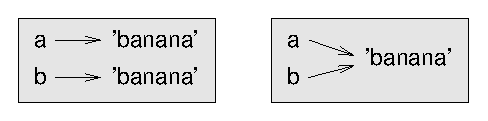
\includegraphics{figs/list1.eps}}
\afterfig

In one case, {\tt a} and {\tt b} refer to two different objects that
have the same value.  In the second case, they refer to the same
object.

\index{is operator}
\index{operator!is}

To check whether two variables refer to the same object, you can
use the {\tt is} operator.

\beforeverb
\begin{verbatim}
>>> a = 'banana'
>>> b = 'banana'
>>> a is b
True
\end{verbatim}
\afterverb
%
In this example, Python only created one string object,
and both {\tt a} and {\tt b} refer to it.

But when you create two lists, you get two objects:

\beforeverb
\begin{verbatim}
>>> a = [1, 2, 3]
>>> b = [1, 2, 3]
>>> a is b
False
\end{verbatim}
\afterverb
%
So the state diagram looks like this:

\index{state diagram}
\index{diagram!state}

\beforefig
\centerline{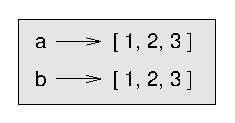
\includegraphics{figs/list2.eps}}
\afterfig

In this case we would say that the two lists are {\bf equivalent},
because they have the same elements, but not {\bf identical}, because
they are not the same object.  If two objects are identical, they are
also equivalent, but if they are equivalent, they are not necessarily
identical.

\index{equivalence}
\index{identity}

Until now, we have been using ``object'' and ``value''
interchangeably, but it is more precise to say that an object has a
value.  If you execute {\tt a = [1,2,3]}, {\tt a} refers to a list
object whose value is a particular sequence of elements.  If another
list has the same elements, we would say it has the same value.

\index{object}
\index{value}


\section{Aliasing}

\index{aliasing}
\index{reference!aliasing}

If {\tt a} refers to an object and you assign {\tt b = a},
then both variables refer to the same object:

\beforeverb
\begin{verbatim}
>>> a = [1, 2, 3]
>>> b = a
>>> b is a
True
\end{verbatim}
\afterverb
%
The state diagram looks like this:

\index{state diagram}
\index{diagram!state}

\beforefig
\centerline{
\includegraphics{figs/list3.eps}}
\afterfig

The association of a variable with an object is called a {\bf
reference}.  In this example, there are two references to the same
object.

\index{reference}

An object with more than one reference has more
than one name, so we say that the object is {\bf aliased}.

\index{mutability}

If the aliased object is mutable, 
changes made with one alias affect
the other:

\beforeverb
\begin{verbatim}
>>> b[0] = 17
>>> print a
[17, 2, 3]
\end{verbatim}
\afterverb
%
Although this behavior can be useful, it is error-prone.  In general,
it is safer to avoid aliasing when you are working with mutable
objects.

\index{immutability}

For immutable objects like strings, aliasing is not as much of a
problem.  In this example:

\beforeverb
\begin{verbatim}
a = 'banana'
b = 'banana'
\end{verbatim}
\afterverb
%
It almost never makes a difference whether {\tt a} and {\tt b} refer
to the same string or not.


\section{List arguments}

\index{list!as argument}
\index{argument}
\index{argument!list}
\index{reference}
\index{parameter}

When you pass a list to a function, the function gets a reference
to the list.
If the function modifies a list parameter, the caller sees the change.
For example, \verb"delete_head" removes the first element from a list:

\beforeverb
\begin{verbatim}
def delete_head(t):
    del t[0]
\end{verbatim}
\afterverb
%
Here's how it is used:

\beforeverb
\begin{verbatim}
>>> letters = ['a', 'b', 'c']
>>> delete_head(letters)
>>> print letters
['b', 'c']
\end{verbatim}
\afterverb
%
The parameter {\tt t} and the variable {\tt letters} are
aliases for the same object.  The stack diagram looks like
this:

\index{stack diagram}
\index{diagram!stack}

\beforefig
\centerline{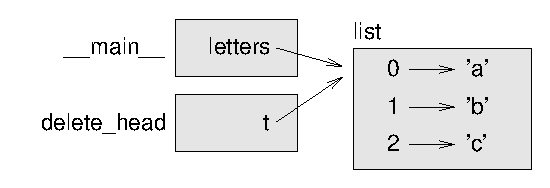
\includegraphics{figs/stack5.eps}}
\afterfig

Since the list is shared by two frames, I drew
it between them.

It is important to distinguish between operations that
modify lists and operations that create new lists.  For
example, the {\tt append} method modifies a list, but the
{\tt +} operator creates a new list:

\index{append method}
\index{method!append}
\index{list!concatenation}
\index{concatenation!list}

\beforeverb
\begin{verbatim}
>>> t1 = [1, 2]
>>> t2 = t1.append(3)
>>> print t1
[1, 2, 3]
>>> print t2
None

>>> t3 = t1 + [3]
>>> print t3
[1, 2, 3]
>>> t2 is t3
False
\end{verbatim}
\afterverb

This difference is important when you write functions that
are supposed to modify lists.  For example, this function
\emph{does not} delete the head of a list:

\beforeverb
\begin{verbatim}
def bad_delete_head(t):
    t = t[1:]              # WRONG!
\end{verbatim}
\afterverb

The slice operator creates a new list and the assignment
makes {\tt t} refer to it, but none of that has any effect
on the list that was passed as an argument.

\index{slice operator}
\index{operator!slice}

An alternative is to write a function that creates and
returns a new list.  For
example, {\tt tail} returns all but the first
element of a list:

\beforeverb
\begin{verbatim}
def tail(t):
    return t[1:]
\end{verbatim}
\afterverb
%
This function leaves the original list unmodified.
Here's how it is used:

\beforeverb
\begin{verbatim}
>>> letters = ['a', 'b', 'c']
>>> rest = tail(letters)
>>> print rest
['b', 'c']
\end{verbatim}
\afterverb


\begin{ex}

Write a function called {\tt chop} that takes a list and modifies
it, removing the first and last elements, and returns {\tt None}.

Then write a function called {\tt middle} that takes a list and
returns a new list that contains all but the first and last
elements.

\end{ex}


\section{Debugging}
\index{debugging}

Careless use of lists (and other mutable objects)
can lead to long hours of debugging.  Here are some common
pitfalls and ways to avoid them:

\begin{enumerate}

\item Don't forget that most list methods modify the argument and
  return {\tt None}.  This is the opposite of the string methods,
  which return a new string and leave the original alone.

If you are used to writing string code like this:

\beforeverb
\begin{verbatim}
word = word.strip()
\end{verbatim}
\afterverb

It is tempting to write list code like this:

\beforeverb
\begin{verbatim}
t = t.sort()           # WRONG!
\end{verbatim}
\afterverb

\index{sort method}
\index{method!sort}

Because {\tt sort} returns {\tt None}, the
next operation you perform with {\tt t} is likely to fail.

Before using list methods and operators, you should read the
documentation carefully and then test them in interactive mode.  The
methods and operators that lists share with other sequences (like
strings) are documented at
\url{docs.python.org/lib/typesseq.html}.  The
methods and operators that only apply to mutable sequences
are documented at \url{docs.python.org/lib/typesseq-mutable.html}.


\item Pick an idiom and stick with it.

Part of the problem with lists is that there are too many
ways to do things.  For example, to remove an element from
a list, you can use {\tt pop}, {\tt remove}, {\tt del},
or even a slice assignment.

To add an element, you can use the {\tt append} method or
the {\tt +} operator.  But don't forget that these are right: 

\beforeverb
\begin{verbatim}
t.append(x)
t = t + [x]
\end{verbatim}
\afterverb

And these are wrong:

\beforeverb
\begin{verbatim}
t.append([x])          # WRONG!
t = t.append(x)        # WRONG!
t + [x]                # WRONG!
t = t + x              # WRONG!
\end{verbatim}
\afterverb

Try out each of these examples in interactive mode to make sure
you understand what they do.  Notice that only the last
one causes a runtime error; the other three are legal, but they
do the wrong thing.


\item Make copies to avoid aliasing.

\index{aliasing!copying to avoid}
\index{copy!to avoid aliasing}

If you want to use a method like {\tt sort} that modifies
the argument, but you need to keep the original list as
well, you can make a copy.

\beforeverb
\begin{verbatim}
orig = t[:]
t.sort()
\end{verbatim}
\afterverb

In this example you could also use the built-in function {\tt sorted},
which returns a new, sorted list and leaves the original alone.
But in that case you should avoid using {\tt sorted} as a variable
name!

\item Lists, {\tt split}, and files

When we read and parse files, there are many opportunities
to encounter input that can crash our program so it is a good 
idea to revisit the {\bf guardian} pattern when it comes
writing programs that read through a file 
and look for a ``needle in the haystack''.

Let's revisit our program that is looking for the day of the
week on the from lines of our file:

{\tt
From stephen.marquard@uct.ac.za {\bf Sat} Jan  5 09:14:16 2008
}

Since we are breaking this line into words, we could dispense
with the use of {\tt startswith} and simply look at the 
first word of the line to determine if we are interested
in the line at all.  We can use {\tt continue} to skip lines
that don't have ``From'' as the first word as follows:

\beforeverb
\begin{verbatim}
fhand = open('mbox-short.txt')
for line in fhand:
    words = line.split()
    if words[0] != 'From' : continue
    print words[2]
\end{verbatim}
\afterverb
%
This looks much simpler and we don't even need to do the 
{\tt rstrip} to remove the newline at the end of the file.
But is it better?

\beforeverb
\begin{verbatim}
python search8.py 
Sat
Traceback (most recent call last):
  File "search8.py", line 5, in <module>
    if words[0] != 'From' : continue
IndexError: list index out of range
\end{verbatim}
\afterverb
%
It kind of works and we see the day from the first line
(Sat) but then the program fails with a traceback error.
What went wrong?  What messed-up data caused our elegant, 
clever and very Pythonic program to fail?

You could stare at it for a long time and puzzle through
it or ask someone for help, but the quicker and smarter
approach is to add a {\tt print} statement.  The best place
to add the print statement is right before the line where
the program failed and print out the data that seems to be causing
the failure.

Now this approach may generate a lot of lines of output but at 
least you will immediately have some clue as to the 
problem at hand.  So we add a print of the variable
{\tt words} right before line five.  We even 
add a prefix ``Debug:'' to the line so we can keep
our regular output separate from our debug output.

\beforeverb
\begin{verbatim}
for line in fhand:
    words = line.split()
    print 'Debug:', words
    if words[0] != 'From' : continue
    print words[2]
\end{verbatim}
\afterverb
%
When we run the program, a lot of output scrolls off the screen
but at the end, we see our debug output and the traceback so 
we know what happened just before the traceback.

\beforeverb
\begin{verbatim}
Debug: ['X-DSPAM-Confidence:', '0.8475']
Debug: ['X-DSPAM-Probability:', '0.0000']
Debug: []
Traceback (most recent call last):
  File "search9.py", line 6, in <module>
    if words[0] != 'From' : continue
IndexError: list index out of range
\end{verbatim}
\afterverb
%
Each debug line is printing the list of words which we get
when we {\tt split} the line into words.  When the program fails
the list of words is empty \verb"[]".  If we open the file in a text editor
and look at the file, at that point it looks as follows:

\beforeverb
\begin{verbatim}
X-DSPAM-Result: Innocent
X-DSPAM-Processed: Sat Jan  5 09:14:16 2008
X-DSPAM-Confidence: 0.8475
X-DSPAM-Probability: 0.0000

Details: http://source.sakaiproject.org/viewsvn/?view=rev&rev=39772
\end{verbatim}
\afterverb
%
The error occurs when our program encounters a blank line! Of course there
are ``zero words'' on a blank line.  Why didn't we think of that 
when we were writing the code.  When the code looks for the first
word (\verb"word[0]") to check to see if it matches ``From'', 
we get an ``index out of range'' error.

This of course is the perfect place to add some {\bf guardian} code 
to avoid checking the first word if the first word is not there.
There are many ways to protect this code, we will choose to 
check the number of words we have before we look at the first word:

\beforeverb
\begin{verbatim}
fhand = open('mbox-short.txt')
count = 0
for line in fhand:
    words = line.split()
    # print 'Debug:', words
    if len(words) == 0 : continue
    if words[0] != 'From' : continue
    print words[2]
\end{verbatim}
\afterverb
%
First we commented out the debug print statement instead of removing it 
in case our modification fails and we need to debug again.  Then we added
a guardian statement that checks to see if we have zero words, and if so, 
we use {\tt continue} to skip to the next line in the file.

We can think of the two {\tt continue} statements as helping us refine
the set of lines which are ``interesting'' to us and which we want 
to process some more.  A line which has no words is ``uninteresting'' to 
us so we skip to the next line.  A line which does not have ``From''
as its first word is uninteresting to us so we skip it.

The program as modified runs successfully so perhaps it is correct.  Our
guardian statement does make sure that the {\tt words[0]} will never fail, 
but perhaps it is not enough.  When we are programming, we must always be 
thinking, ``What might go wrong?''.

\begin{ex}
Figure out which line of the above program is still not properly guarded.
See if you can construct a text file which causes the program to fail
and then modify the program so that the line is properly guarded and 
test it to make sure it handles your new text file.
\end{ex}

\begin{ex}
Rewrite the guardian code in the above example without two
{\tt if} statements.  Instead use a compound logical expression using the
{\tt and} logical operator with a single {\tt if} statement.
\end{ex}


\end{enumerate}



\section{Glossary}

\begin{description}

\item[aliasing:] A circumstance where two or more variables refer to the same
object.
\index{aliasing}

\item[delimiter:] A character or string used to indicate where a
string should be split.
\index{delimiter}

\item[element:] One of the values in a list (or other sequence),
also called items.
\index{element}

\item[equivalent:] Having the same value.
\index{equivalent}

\item[index:] An integer value that indicates an element in a list.
\index{index}

\item[identical:] Being the same object (which implies equivalence).
\index{identical}

\item[list:] A sequence of values.
\index{list}

\item[list traversal:] The sequential accessing of each element in a list.
\index{list!traversal}

\item[nested list:] A list that is an element of another list.
\index{nested list}

\item[object:] Something a variable can refer to.  An object
has a type and a value.
\index{object}

\item[reference:] The association between a variable and its value.
\index{reference}

\end{description}


\section{Exercises}

\begin{ex}
Download a copy of the file from 
\url{www.py4inf.com/code/romeo.txt}

Write a program to open the file {\tt romeo.txt} and read it
line by line.  For each line, split the line into  a list of 
words using the {\tt split} function.

For each word, check to see if the word is already in a list.  
If the word is not in the list, add it to the list.  

When the program completes, sort and print the resulting words
in alphabetical order.

\begin{verbatim}
Enter file: romeo.txt
['Arise', 'But', 'It', 'Juliet', 'Who', 'already', 
'and', 'breaks', 'east', 'envious', 'fair', 'grief', 
'is', 'kill', 'light', 'moon', 'pale', 'sick', 'soft', 
'sun', 'the', 'through', 'what', 'window', 
'with', 'yonder']
\end{verbatim}
\end{ex}

\begin{ex}
Write a program to read through the mail box data and when you find 
line that starts with ``From'', you will split the line into 
words using the {\tt split} function. We are interested in 
who sent the message which is the second word on the From line.

{\tt From stephen.marquard@uct.ac.za Sat Jan  5 09:14:16 2008 }

You will parse the From line and print out the second word for 
each From line and then you will also count the number of 
From (not From:) lines and print out a count at the end.

This is a sample good output with a few lines removed:

\beforeverb
\begin{verbatim}
python fromcount.py 
Enter a file name: mbox-short.txt
stephen.marquard@uct.ac.za
louis@media.berkeley.edu
zqian@umich.edu

[...some output removed...]

ray@media.berkeley.edu
cwen@iupui.edu
cwen@iupui.edu
cwen@iupui.edu
There were 27 lines in the file with From as the first word
\end{verbatim}
\afterverb
%
\end{ex}

\begin{ex}
Rewrite the program that prompts the user for a list of 
numbers and prints out the maximum and minimum of the
numbers at the end when the user enters ``done''.  Write
the program to store the numbers the user enters in a list
and use the {\tt max()} and {\tt min()} fuctions to 
compute the maximum and minimum numbers after the 
loop completes.

\beforeverb
\begin{verbatim}
Enter a number: 6
Enter a number: 2
Enter a number: 9
Enter a number: 3
Enter a number: 5
Enter a number: done
Maximum: 9.0
Minimum: 2.0
\end{verbatim}
\afterverb
%

\end{ex}

\chapter{Dictionaries}
\index{dictionary}

\index{dictionary}
\index{type!dict}
\index{key}
\index{key-value pair}
\index{index}

A {\bf dictionary} is like a list, but more general.  In a list,
the positions (a.k.a. indices) have to be integers; in a dictionary 
the indices can be (almost) any type.

You can think of a dictionary as a mapping between a set of indices
(which are called {\bf keys}) and a set of values.  Each key maps to a
value.  The association of a key and a value is called a {\bf
  key-value pair} or sometimes an {\bf item}.

As an example, we'll build a dictionary that maps from English
to Spanish words, so the keys and the values are all strings.

The function {\tt dict} creates a new dictionary with no items.
Because {\tt dict} is the name of a built-in function, you
should avoid using it as a variable name.

\index{dict function}
\index{function!dict}

\beforeverb
\begin{verbatim}
>>> eng2sp = dict()
>>> print eng2sp
{}
\end{verbatim}
\afterverb

The squiggly-brackets, \verb"{}", represent an empty dictionary.
To add items to the dictionary, you can use square brackets:

\index{squiggly bracket}
\index{bracket!squiggly}

\beforeverb
\begin{verbatim}
>>> eng2sp['one'] = 'uno'
\end{verbatim}
\afterverb
%
This line creates an item that maps from the key
{\tt 'one'} to the value \verb"'uno'".  If we print the
dictionary again, we see a key-value pair with a colon
between the key and value:

\beforeverb
\begin{verbatim}
>>> print eng2sp
{'one': 'uno'}
\end{verbatim}
\afterverb
%
This output format is also an input format.  For example,
you can create a new dictionary with three items:

\beforeverb
\begin{verbatim}
>>> eng2sp = {'one': 'uno', 'two': 'dos', 'three': 'tres'}
\end{verbatim}
\afterverb
%
But if you print {\tt eng2sp}, you might be surprised:

\beforeverb
\begin{verbatim}
>>> print eng2sp
{'one': 'uno', 'three': 'tres', 'two': 'dos'}
\end{verbatim}
\afterverb
%
The order of the key-value pairs is not the same.  In fact, if
you type the same example on your computer, you might get a
different result.  In general, the order of items in
a dictionary is unpredictable.

But that's not a problem because
the elements of a dictionary are never indexed with integer indices.
Instead, you use the keys to look up the corresponding values:

\beforeverb
\begin{verbatim}
>>> print eng2sp['two']
'dos'
\end{verbatim}
\afterverb
%
The key {\tt 'two'} always maps to the value \verb"'dos'" so the order
of the items doesn't matter.

If the key isn't in the dictionary, you get an exception:

\index{exception!KeyError}
\index{KeyError}

\beforeverb
\begin{verbatim}
>>> print eng2sp['four']
KeyError: 'four'
\end{verbatim}
\afterverb
%
The {\tt len} function works on dictionaries; it returns the
number of key-value pairs:

\index{len function}
\index{function!len}

\beforeverb
\begin{verbatim}
>>> len(eng2sp)
3
\end{verbatim}
\afterverb
%
The {\tt in} operator works on dictionaries; it tells you whether
something appears as a \emph{key} in the dictionary (appearing
as a value is not good enough).

\index{membership!dictionary}
\index{in operator}
\index{operator!in}

\beforeverb
\begin{verbatim}
>>> 'one' in eng2sp
True
>>> 'uno' in eng2sp
False
\end{verbatim}
\afterverb
%
To see whether something appears as a value in a dictionary, you
can use the method {\tt values}, which returns the values as
a list, and then use the {\tt in} operator:

\index{values method}
\index{method!values}

\beforeverb
\begin{verbatim}
>>> vals = eng2sp.values()
>>> 'uno' in vals
True
\end{verbatim}
\afterverb
%
The {\tt in} operator uses different algorithms for lists and
dictionaries.  For lists, it uses a linear search algorithm.
As the list gets longer, the search time gets
longer in direct proportion to the length of the list.  
For dictionaries, Python uses an
algorithm called a {\bf hash table} that has a remarkable property; the
{\tt in} operator takes about the same amount of time no matter how
many items there are in a dictionary.  I won't explain 
why hash functions are so magical,
but you can read more about it at
\url{wikipedia.org/wiki/Hash_table}.

\index{hash table}

\begin{ex}
\label{wordlist2}

\index{set membership}
\index{membership!set}

Write a function that reads the words in {\tt words.txt} and
stores them as keys in a dictionary.  It doesn't matter what the
values are.  Then you can use the {\tt in} operator
as a fast way to check whether a string is in
the dictionary.

\end{ex}


\section{Dictionary as a set of counters}
\label{histogram}

\index{counter}

Suppose you are given a string and you want to count how many
times each letter appears.  There are several ways you could do it:

\begin{enumerate}

\item You could create 26 variables, one for each letter of the
alphabet.  Then you could traverse the string and, for each
character, increment the corresponding counter, probably using
a chained conditional.

\item You could create a list with 26 elements.  Then you could
convert each character to a number (using the built-in function
{\tt ord}), use the number as an index into the list, and increment
the appropriate counter.

\item You could create a dictionary with characters as keys
and counters as the corresponding values.  The first time you
see a character, you would add an item to the dictionary.  After
that you would increment the value of an existing item.

\end{enumerate}

Each of these options performs the same computation, but each
of them implements that computation in a different way.

\index{implementation}

An {\bf implementation} is a way of performing a computation;
some implementations are better than others.  For example,
an advantage of the dictionary implementation is that we don't
have to know ahead of time which letters appear in the string
and we only have to make room for the letters that do appear.

Here is what the code might look like:

\beforeverb
\begin{verbatim}
def histogram(s):
    d = dict()
    for c in s:
        if c not in d:
            d[c] = 1
        else:
            d[c] = d[c] + 1
    return d
\end{verbatim}
\afterverb
%
The name of the function is {\bf histogram}, which is a statistical
term for a set of counters (or frequencies).  

\index{histogram}
\index{frequency}
\index{traversal}

The first line of the
function creates an empty dictionary.  The {\tt for} loop traverses
the string.  Each time through the loop, if the character {\tt c} is
not in the dictionary, we create a new item with key {\tt c} and the
initial value 1 (since we have seen this letter once).  If {\tt c} is
already in the dictionary we increment {\tt d[c]}.

\index{histogram}

Here's how it works:

\beforeverb
\begin{verbatim}
>>> h = histogram('brontosaurus')
>>> print h
{'a': 1, 'b': 1, 'o': 2, 'n': 1, 's': 2, 'r': 2, 'u': 2, 't': 1}
\end{verbatim}
\afterverb
%
The histogram indicates that the letters {\tt 'a'} and \verb"'b'"
appear once; \verb"'o'" appears twice, and so on.

\begin{ex}

\index{get method}
\index{method!get}

Dictionaries have a method called {\tt get} that takes a key
and a default value.  If the key appears in the dictionary,
{\tt get} returns the corresponding value; otherwise it returns
the default value.  For example:

\beforeverb
\begin{verbatim}
>>> h = histogram('a')
>>> print h
{'a': 1}
>>> h.get('a', 0)
1
>>> h.get('b', 0)
0
\end{verbatim}
\afterverb
%
Use {\tt get} to write {\tt histogram} more concisely.  You
should be able to eliminate the {\tt if} statement.
\end{ex}

\section{Dictionaries and files}

One of the common uses of a dictionary is to count the occurrence
of words in a file with some written text.  
Let's start with a very simple file of
words taken from the text of \emph{Romeo and Juliet}
thanks to 
\url{http://shakespeare.mit.edu/Tragedy/romeoandjuliet/romeo_juliet.2.2.html}.

For the first set of examples, we will use a shortened and simplified version
of the text with no punctuation.  Later we will work with the text of the 
scene with punctuation included.

\beforeverb
\begin{verbatim}
But soft what light through yonder window breaks
It is the east and Juliet is the sun
Arise fair sun and kill the envious moon
Who is already sick and pale with grief
\end{verbatim}
\afterverb
%
We will write a Python program to read through the lines of the file, 
break each line into a list of words, and then loop through each 
of the words in the line, and count each word using a dictionary.

\index{nested loops}
\index{loop!nested}
You will see that we have two {\tt for} loops.  The outer loop is reading the
lines of the file and the inner loop is iterating through each
of the words on that particular line.  This is an example
of a pattern called {\bf nested loops} because one of the loops
is the \emph{outer} loop and the other loop is the \emph{inner}
loop.  

Because the inner loop executes all of its iterations each time
the outer loop makes a single iteration, we think of the inner
loop as iterating ``more quickly'' and the outer loop as iterating 
more slowly.

The combination of the two nested loops ensures that we will count
every word on every line of the input file.

\beforeverb
\begin{verbatim}
fname = raw_input('Enter the file name: ')
try:
    fhand = open(fname)
except:
    print 'File cannot be opened:', fname
    exit()

counts = dict()
for line in fhand:
    words = line.split()
    for word in words:
        if word not in counts:
            counts[word] = 1
        else:
            counts[word] += 1

print counts
\end{verbatim}
\afterverb
%
When we run the program, we see a raw dump of all of the counts in unsorted
hash order.
(the {\tt romeo.txt} file is available at
\url{www.py4inf.com/code/romeo.txt})

\beforeverb
\begin{verbatim}
python count1.py 
Enter the file name: romeo.txt
{'and': 3, 'envious': 1, 'already': 1, 'fair': 1, 
'is': 3, 'through': 1, 'pale': 1, 'yonder': 1, 
'what': 1, 'sun': 2, 'Who': 1, 'But': 1, 'moon': 1, 
'window': 1, 'sick': 1, 'east': 1, 'breaks': 1, 
'grief': 1, 'with': 1, 'light': 1, 'It': 1, 'Arise': 1, 
'kill': 1, 'the': 3, 'soft': 1, 'Juliet': 1}
\end{verbatim}
\afterverb
%
It is a bit inconvenient to look through the dictionary to find the
most common words and their counts, so we need to add some more 
Python code to get us the output that will be more helpful.

\section{Looping and dictionaries}

\index{dictionary!looping with}
\index{looping!with dictionaries}
\index{traversal}

If you use a dictionary as the sequence 
in a {\tt for} statement, it traverses
the keys of the dictionary.  For example, \verb"print_hist"
prints each key and the corresponding value:

\beforeverb
\begin{verbatim}
def print_hist(h):
    for c in h:
        print c, h[c]
\end{verbatim}
\afterverb
%
Here's what the output looks like:

\beforeverb
\begin{verbatim}
>>> h = histogram('parrot')
>>> print_hist(h)
a 1
p 1
r 2
t 1
o 1
\end{verbatim}
\afterverb
%
Again, the keys are in no particular order.

\index{keys method}
\index{method!keys}
If you want to print the keys in alphabetical order, you first 
make a list of the keys in the dictionary using the 
{\tt keys} method available in dictionary objects,
and then sort that list
and loop through the sorted list, looking up each
key printing out key/value pairs in sorted order as follows
as follows:

\beforeverb
\begin{verbatim}
def print_sorted_hist(h):
    lst = h.keys()
    lst.sort()
    for c in lst:
        print c, h[c]
\end{verbatim}
\afterverb
%
Here's what the output looks like:

\beforeverb
\begin{verbatim}
>>> h = histogram('parrot')
>>> print_sorted_hist(h)
a 1
o 1
p 1
r 2
t 1
\end{verbatim}
\afterverb
%
So now the keys are in alphabetical order.

\section{Advanced text parsing}

In the above example using the file {\tt romeo.txt},
we made the file as simple as possible by removing 
any and all punctuation by hand.  The real text 
has lots of punctuation as shown below:

\beforeverb
\begin{verbatim}
But, soft! what light through yonder window breaks?
It is the east, and Juliet is the sun.
Arise, fair sun, and kill the envious moon,
Who is already sick and pale with grief,
\end{verbatim}
\afterverb
%
Since the Python {\tt split} function looks for spaces and
treats words as tokens separated by spaces, we would treat the
words ``soft!'' and ``soft'' as \emph{different} words and create
a separate dictionary entry for each word.

Also since the file has capitalization, we would treat
``who'' and ``Who'' as different words with different 
counts.

We can solve both these problems by using the string
methods {\tt lower}, {\tt punctuation}, and {\tt translate}.  The 
{\tt translate} is the most subtle of the methods.  
Here is the documentation for {\tt translate}:

\verb"string.translate(s, table[, deletechars])"

\emph{Delete all characters from s that are in deletechars (if present), 
and then translate the characters using table, which must 
be a 256-character string giving the translation for each 
character value, indexed by its ordinal. If table is None, 
then only the character deletion step is performed.}

We will not specify the {\tt table} but we will use 
the {\tt deletechars} parameter to delete all of the punctuation.
We will even let Python tell us the list of characters
that it considers ``punctuation'':

\beforeverb
\begin{verbatim}
>>> import string
>>> string.punctuation
'!"#$%&\'()*+,-./:;<=>?@[\\]^_`{|}~'
\end{verbatim}
\afterverb
%
We make the following modifications to our program:

\beforeverb
\begin{verbatim}
import string                                          # New Code

fname = raw_input('Enter the file name: ')
try:
    fhand = open(fname)
except:
    print 'File cannot be opened:', fname
    exit()

counts = dict()
for line in fhand:
    line = line.translate(None, string.punctuation)    # New Code
    line = line.lower()                                # New Code
    words = line.split()
    for word in words:
        if word not in counts:
            counts[word] = 1
        else:
            counts[word] += 1

print counts
\end{verbatim}
\afterverb
%
We use {\tt translate} to remove all punctuation and {\tt lower} to 
force the line to lowercase.  Otherwise the program is unchanged.
Note for Python 2.5 and earlier, {\tt translate} does not 
accept {\tt None} as the first parameter so use this code for the translate 
call:

\beforeverb
\begin{verbatim}
print a.translate(string.maketrans(' ',' '), string.punctuation
\end{verbatim}
\afterverb
%
Part of learning the ``Art of Python'' or ``Thinking Pythonically''
is realizing that Python
often has built-in capabilities for many common data-analysis
problems.  Over time, you will see enough example code and read
enough of the documentation to know where to look to see if someone
has already written something that makes your job much easier.

The following is an abbreviated version of the output:
\beforeverb
\begin{verbatim}
Enter the file name: romeo-full.txt
{'swearst': 1, 'all': 6, 'afeard': 1, 'leave': 2, 'these': 2, 
'kinsmen': 2, 'what': 11, 'thinkst': 1, 'love': 24, 'cloak': 1, 
a': 24, 'orchard': 2, 'light': 5, 'lovers': 2, 'romeo': 40, 
'maiden': 1, 'whiteupturned': 1, 'juliet': 32, 'gentleman': 1, 
'it': 22, 'leans': 1, 'canst': 1, 'having': 1, ...}
\end{verbatim}
\afterverb
%
Looking through this output is still unwieldy and we can use
Python to gives us exactly what we are looking for, but to do 
so, we need to learn about Python {\bf tuples}.  We
will pick up this example once we learn about tuples.

\section{Debugging}
\index{debugging}

As you work with bigger datasets it can become unwieldy to
debug by printing and checking data by hand.  Here are some
suggestions for debugging large datasets:

\begin{description}

\item[Scale down the input:] If possible, reduce the size of the
dataset.  For example if the program reads a text file, start with
just the first 10 lines, or with the smallest example you can find.
You can either edit the files themselves, or (better) modify the
program so it reads only the first {\tt n} lines.

If there is an error, you can reduce {\tt n} to the smallest
value that manifests the error, and then increase it gradually
as you find and correct errors.

\item[Check summaries and types:] Instead of printing and checking the
entire dataset, consider printing summaries of the data: for example,
the number of items in a dictionary or the total of a list of numbers.

A common cause of runtime errors is a value that is not the right
type.  For debugging this kind of error, it is often enough to print
the type of a value.

\item[Write self-checks:]  Sometimes you can write code to check
for errors automatically.  For example, if you are computing the
average of a list of numbers, you could check that the result is
not greater than the largest element in the list or less than
the smallest.  This is called a ``sanity check'' because it detects
results that are ``insane.''

\index{sanity check}
\index{consistency check}

Another kind of check compares the results of two different
computations to see if they are consistent.  This is called a
``consistency check.''

\item[Pretty print the output:] Formatting debugging output
can make it easier to spot an error.  

\end{description}

Again, time you spend building scaffolding can reduce
the time you spend debugging.

\index{scaffolding}

\section{Glossary}

\begin{description}

\item[dictionary:] A mapping from a set of keys to their
corresponding values.
\index{dictionary}

\item[hashtable:] The algorithm used to implement Python
dictionaries.
\index{hashtable}

\item[hash function:] A function used by a hashtable to compute the
location for a key.
\index{hash function}

\item[histogram:] A set of counters.
\index{histogram}

\item[implementation:] A way of performing a computation.
\index{implementation}

\item[item:] Another name for a key-value pair.
\index{item!dictionary}

\item[key:] An object that appears in a dictionary as the
first part of a key-value pair.
\index{key}

\item[key-value pair:] The representation of the mapping from
a key to a value.
\index{key-value pair}

\item[lookup:] A dictionary operation that takes a key and finds
the corresponding value.
\index{lookup}

\item[nested loops:] When there is one or more loops ``inside'' of 
another loop.  The inner loop runs to completion each time the outer
loop runs once.
\index{nested loops}
\index{loop!nested}

\item[value:] An object that appears in a dictionary as the
second part of a key-value pair.  This is more specific than
our previous use of the word ``value.''
\index{value}

\end{description}

\section{Exercises}

\begin{ex}
Write a program that categorizes each mail message by which 
day of the week the commit was done. To do this look for 
lines which start with ``From'', then look for the 
third word and then keep a running count of each of the 
days of the week. At the end of the program print out the 
contents of your dictionary (order does not matter).

\beforeverb
\begin{verbatim}
Sample Line:
From stephen.marquard@uct.ac.za Sat Jan  5 09:14:16 2008

Sample Execution:
python dow.py
Enter a file name: mbox-short.txt
{'Fri': 20, 'Thu': 6, 'Sat': 1}
\end{verbatim}
\afterverb
\end{ex}

\begin{ex}
Write a program to read through a mail log, and figure 
out who had the most messages in the file.  The program looks 
for ``From'' lines and takes the second parameter on those 
lines as the person who sent the mail.

The program creates a Python dictionary that maps 
the sender's address to the total number of messages for that person.

After all the data has been read the program looks 
through the dictionary using a maximum loop
 (see Section~\ref{maximumloop})
to find who has the most 
messages and how many messages the person has.

\beforeverb
\begin{verbatim}
Enter a file name: mbox-short.txt
cwen@iupui.edu 5

Enter a file name: mbox.txt
zqian@umich.edu 195
\end{verbatim}
\afterverb
\end{ex}

\begin{ex}
This program records the domain name (instead of the address) 
where the message was sent from instead of who the mail 
came from (i.e. the whole e-mail address). At the end 
of the program print out the contents of your dictionary. 

\beforeverb
\begin{verbatim}
python schoolcount.py
Enter a file name: mbox-short.txt
{'media.berkeley.edu': 4, 'uct.ac.za': 6, 'umich.edu': 7, 
'gmail.com': 1, 'caret.cam.ac.uk': 1, 'iupui.edu': 8}
\end{verbatim}
\afterverb
\end{ex}

\chapter{Tuples}
\label{tuplechap}

\section{Tuples are immutable}

\index{tuple}
\index{type!tuple}
\index{sequence}

A tuple is a sequence of values much like a list.  
The values stored in a tuple can be any type, and
they are indexed by integers.
The important difference is that tuples are {\bf immutable}.
Tuples are also {\bf comparable} and {\bf hashable} so we can 
sort lists of them and use tuples as key values in Python
dictionaries.

\index{mutability}
\index{hashable}
\index{comparable}
\index{immutability}

Syntactically, a tuple is a comma-separated list of values:

\beforeverb
\begin{verbatim}
>>> t = 'a', 'b', 'c', 'd', 'e'
\end{verbatim}
\afterverb
%
Although it is not necessary, it is common to enclose tuples in
parentheses to help use quickly identify tuples when we look at
Python code:

\index{parentheses!tuples in}

\beforeverb
\begin{verbatim}
>>> t = ('a', 'b', 'c', 'd', 'e')
\end{verbatim}
\afterverb
%
To create a tuple with a single element, you have to include the final
comma:

\index{singleton}
\index{tuple!singleton}

\beforeverb
\begin{verbatim}
>>> t1 = ('a',)
>>> type(t1)
<type 'tuple'>
\end{verbatim}
\afterverb
%
Without the comma Python treats \verb"('a')" as an expression 
with a string in parentheses that evaluates to a string:

\beforeverb
\begin{verbatim}
>>> t2 = ('a')
>>> type(t2)
<type 'str'>
\end{verbatim}
\afterverb
%
Another way to construct a tuple is the built-in function {\tt tuple}.
With no argument, it creates an empty tuple:

\index{tuple function}
\index{function!tuple}

\beforeverb
\begin{verbatim}
>>> t = tuple()
>>> print t
()
\end{verbatim}
\afterverb
%
If the argument is a sequence (string, list or tuple), the result
of the call to {\tt tuple}
is a tuple with the elements of the sequence:

\beforeverb
\begin{verbatim}
>>> t = tuple('lupins')
>>> print t
('l', 'u', 'p', 'i', 'n', 's')
\end{verbatim}
\afterverb
%
Because {\tt tuple} is the name of a constructor, you should
avoid using it as a variable name.

Most list operators also work on tuples.  The bracket operator
indexes an element:

\index{bracket operator}
\index{operator!bracket}

\beforeverb
\begin{verbatim}
>>> t = ('a', 'b', 'c', 'd', 'e')
>>> print t[0]
'a'
\end{verbatim}
\afterverb
%
And the slice operator selects a range of elements.

\index{slice operator}
\index{operator!slice}
\index{tuple!slice}
\index{slice!tuple}

\beforeverb
\begin{verbatim}
>>> print t[1:3]
('b', 'c')
\end{verbatim}
\afterverb
%
But if you try to modify one of the elements of the tuple, you get
an error:

\index{exception!TypeError}
\index{TypeError}
\index{item assignment}
\index{assignment!item}

\beforeverb
\begin{verbatim}
>>> t[0] = 'A'
TypeError: object doesn't support item assignment
\end{verbatim}
\afterverb
%
You can't modify the elements of a tuple, but you can replace
one tuple with another:

\beforeverb
\begin{verbatim}
>>> t = ('A',) + t[1:]
>>> print t
('A', 'b', 'c', 'd', 'e')
\end{verbatim}
\afterverb
%

\section{Comparing tuples}

\index{comparison!tuple}
\index{tuple!comparison}
\index{sort method}
\index{method!sort}

The comparison operators work with tuples and other sequences;
Python starts by comparing the first element from each
sequence.  If they are equal, it goes on to the next element,
and so on, until it finds elements that differ.  Subsequent
elements are not considered (even if they are really big).

\beforeverb
\begin{verbatim}
>>> (0, 1, 2) < (0, 3, 4)
True
>>> (0, 1, 2000000) < (0, 3, 4)
True
\end{verbatim}
\afterverb
%
The {\tt sort} function works the same way.  It sorts 
primarily by first element, but in the case of a tie, it sorts
by second element, and so on.  

This feature lends itself to a pattern called {\bf DSU} for 

\begin{description}

\item[Decorate] a sequence by building a list of tuples
with one or more sort keys preceding the elements from the sequence,

\item[Sort] the list of tuples uring the Python built-in {\tt sort}, and

\item[Undecorate] by extracting the sorted elements of the sequence.

\end{description}

\label{DSU}
\index{DSU pattern}
\index{pattern!DSU}
\index{decorate-sort-undecorate pattern}
\index{pattern!decorate-sort-undecorate}

For example, suppose you have a list of words and you want to
sort them from longest to shortest:

\beforeverb
\begin{verbatim}
def sort_by_length(words):
    t = list()
    for word in words:
       t.append((len(word), word))

    t.sort(reverse=True)

    res = list()
    for length, word in t:
        res.append(word)
    return res
\end{verbatim}
\afterverb
%
The first loop builds a list of tuples, where each
tuple is a word preceded by its length.

{\tt sort} compares the first element, length, first, and
only considers the second element to break ties.  The keyword argument
{\tt reverse=True} tells {\tt sort} to go in decreasing order.

\index{keyword argument}
\index{argument!keyword}
\index{traversal}

The second loop traverses the list of tuples and builds a list of
words in descending order of length.


\section{Tuple assignment}
\label{tuple assignment}

\index{tuple!assignment}
\index{assignment!tuple}
\index{swap pattern}
\index{pattern!swap}

One of the unique syntactic features of the Python language
is the ability to have a tuple on the left hand
side of an assignment statement.  This allows you to assign
more than one variable at a time when the left hand side is a 
sequence.

In this example we have a two element list (which is a sequence) and
assign the first and second elements of the sequence
to the variables {\tt x} and {\tt y} in a single statement.

\beforeverb
\begin{verbatim}
>>> m = [ 'have', 'fun' ]
>>> x, y = m
>>> x
'have'
>>> y
'fun'
>>> 
\end{verbatim}
\afterverb
%
It is not magic, Python \emph{roughly} translates the 
tuple assignment syntax
to be the following:\footnote{Python does not translate the 
syntax literally.  For example if you try this with a dictionary
it will not work as might expect.}

\beforeverb
\begin{verbatim}
>>> m = [ 'have', 'fun' ]
>>> x = m[0]
>>> y = m[1]
>>> x
'have'
>>> y
'fun'
>>> 
\end{verbatim}
\afterverb

Stylistically when we use a tuple on the left hand side of the assignment
statement, we omit the parentheses, but the following is an equally 
valid syntax:

\beforeverb
\begin{verbatim}
>>> m = [ 'have', 'fun' ]
>>> (x, y) = m
>>> x
'have'
>>> y
'fun'
>>> 
\end{verbatim}
\afterverb
%
A particularly clever application of tuple assignment allows
us to {\bf swap} the values of two variables in a single statement:

\beforeverb
\begin{verbatim}
>>> a, b = b, a
\end{verbatim}
\afterverb
%
Both sides of this statement are tuples, but
the left side is a tuple of variables; the right side is a tuple of
expressions.  Each value on the right side 
is assigned to its respective variable on the left side.  
All the expressions on the right side are evaluated before any
of the assignments.

The number of variables on the left and the number of
values on the right have to be the same:

\index{exception!ValueError}
\index{ValueError}

\beforeverb
\begin{verbatim}
>>> a, b = 1, 2, 3
ValueError: too many values to unpack
\end{verbatim}
\afterverb
%
More generally, the right side can be any kind of sequence
(string, list or tuple).  For example, to split an email address
into a user name and a domain, you could write:

\index{split method}
\index{method!split}
\index{email address}

\beforeverb
\begin{verbatim}
>>> addr = 'monty@python.org'
>>> uname, domain = addr.split('@')
\end{verbatim}
\afterverb
%
The return value from {\tt split} is a list with two elements;
the first element is assigned to {\tt uname}, the second to
{\tt domain}.

\beforeverb
\begin{verbatim}
>>> print uname
monty
>>> print domain
python.org
\end{verbatim}
\afterverb
%

\section{Dictionaries and tuples}

\index{dictionary}
\index{items method}
\index{method!items}
\index{key-value pair}

Dictionaries have a method called {\tt items} that returns a list of
tuples, where each tuple is a key-value 
pair\footnote{This behavior is slightly different in Python 3.0.}.

\beforeverb
\begin{verbatim}
>>> d = {'a':10, 'b':1, 'c':22}
>>> t = d.items()
>>> print t
[('a', 10), ('c', 22), ('b', 1)]
\end{verbatim}
\afterverb
%
As you should expect from a dictionary, the items are in no
particular order.

However, since the list of tuples is a list, and tuples are comparable,
we can now sort the list of tuples.  Converting a dictionary
to a list of tuples is a way for us to output the contents of a 
dictionary sorted by key:

\beforeverb
\begin{verbatim}
>>> d = {'a':10, 'b':1, 'c':22}
>>> t = d.items()
>>> t
[('a', 10), ('c', 22), ('b', 1)]
>>> t.sort()
>>> t
[('a', 10), ('b', 1), ('c', 22)]
\end{verbatim}
\afterverb
%
The new list is sorted in ascending alphabetical order by the key value.

\section{Multiple assignment with dictionaries}

\index{traverse!dictionary}
\index{dictionary!traversal}

Combining {\tt items}, tuple assignment and {\tt for}, you
can see a nice code pattern for traversing the keys and values of a dictionary
in a single loop:

\beforeverb
\begin{verbatim}
for key, val in d.items():
    print val, key
\end{verbatim}
\afterverb
%
This loop has two {\bf iteration variables} because {\tt items} returns
a list of tuples and {\tt key, val} is a tuple assignment
that successively iterates through each of the key/value pairs in the dictionary.  

For each iteration
through the loop, both {\tt key} and {\tt value} are advanced to the
next key/value pair in the dictionary (still in hash order).

The output of this loop is:

\beforeverb
\begin{verbatim}
0 a
2 c
1 b
\end{verbatim}
\afterverb
%
Again in hash key order (i.e. no particular order).

If we combine these two techniques, we can print out the contents
of a dictionary sorted by the \emph{value} stored in each key/value
pair.

To do this, we first make a list of tuples where each tuple is 
{\tt (value, key)}.  The {\tt items} method would give us a list of 
{\tt (key, value)} tuples--but this time we want to sort by value not key.
Once we have constructed the list with the value/key tuples, it is a simple
matter to sort the list in reverse order and print out the new, sorted list.

\beforeverb
\begin{verbatim}
>>> d = {'a':10, 'b':1, 'c':22}
>>> l = list()
>>> for key, val in d.items() :
...     l.append( (val, key) )
... 
>>> l
[(10, 'a'), (22, 'c'), (1, 'b')]
>>> l.sort(reverse=True)
>>> l
[(22, 'c'), (10, 'a'), (1, 'b')]
>>> 
\end{verbatim}
\afterverb
%
By hand-constructing the list of tuples to have the value as the first
element of each tuple, we can sort the list of tuples and get our dictionary
contents sorted by value.

\section{The most common words}

Coming back to our running example of the text from \emph{Romeo and Juliet} 
Act 2, Scene 2, we can augment our program to use this technique to 
print the ten most common words in the text as follows:

\beforeverb
\begin{verbatim}
import string
fhand = open('romeo-full.txt')
counts = dict()
for line in fhand:
    line = line.translate(None, string.punctuation)
    line = line.lower()
    words = line.split()
    for word in words:
        if word not in counts:
            counts[word] = 1
        else:
            counts[word] += 1

# Sort the dictionary by value
lst = list()
for key, val in counts.items():
    lst.append( (val, key) )

lst.sort(reverse=True)

for key, val in lst[:10] :
    print key, val
\end{verbatim}
\afterverb
%
The first part of the program which reads the file and computes 
the dictionary that maps each word to the count of words in the 
document is unchanged.  But instead of simply printing out 
{\tt counts} and ending the program, we construct a list 
of {\tt (val, key)} tuples and then sort the list in reverse order.

Since the value is first, it will be used for the comparisons and 
if there is more than one tuple with the same value, it will look
at the second element (the key) so tuples where the value is the
same will be further sorted by the alphabetical order of the key.

At the end we write a nice {\t for loop} which does a multiple
assignment iteration and prints out the ten most common words
by iterating through a slice of the list ({\tt lst[:10]}).

So now the output finally looks like what we want for our word 
frequency analysis.

\beforeverb
\begin{verbatim}
61 i
42 and
40 romeo
34 to
34 the
32 thou
32 juliet
30 that
29 my
24 thee
\end{verbatim}
\afterverb
%
The fact that this relatively complex data parsing and analysis 
can be done with a relatively easy-to-understand 19 line Python
program is one reason why Python is a good choice as a language 
for exploring information.

\section{Using tuples as keys in dictionaries}

\index{tuple!as key in dictionary}
\index{hashable}

Because tuples are {\bf hashable} and lists are not, if we want to 
create a {\bf composite} key to use in a dictionary we must use a tuple as
the key.

We would encounter a composite key if we wanted to create a 
telephone directory that maps
from last-name, first-name pairs to telephone numbers.  Assuming
that we have defined the variables 
{\tt last}, {\tt first} and {\tt number}, we could write
a dictionary assignment statement as follows:

\beforeverb
\begin{verbatim}
directory[last,first] = number
\end{verbatim}
\afterverb
%
The expression in brackets is a tuple.  We could use tuple
assignment in a {\tt for} loop to traverse this dictionary.

\index{tuple!in brackets}

\beforeverb
\begin{verbatim}
for last, first in directory:
    print first, last, directory[last,first]
\end{verbatim}
\afterverb
%
This loop traverses the keys in {\tt directory}, which are tuples.  It
assigns the elements of each tuple to {\tt last} and {\tt first}, then
prints the name and corresponding telephone number.

There are two ways to represent tuples in a state diagram.  The more
detailed version shows the indices and elements just as they appear in
a list.  For example, the tuple \verb"('Cleese', 'John')" would appear:

\index{state diagram}
\index{diagram!state}

\beforefig
\centerline{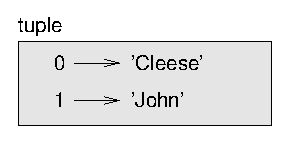
\includegraphics{figs/tuple1.eps}}
\afterfig

But in a larger diagram you might want to leave out the
details.  For example, a diagram of the telephone directory might
appear:

\beforefig
\centerline{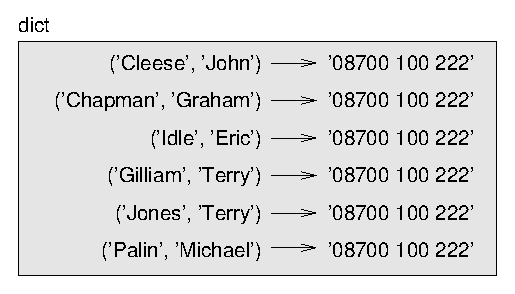
\includegraphics{figs/dict2.eps}}
\afterfig

Here the tuples are shown using Python syntax as a graphical
shorthand.

The telephone number in the diagram is the complaints line for the
BBC, so please don't call it.

\section{Sequences: strings, lists, and tuples--Oh My!}
\index{sequence}

I have focused on lists of tuples, but almost all of the examples in
this chapter also work with lists of lists, tuples of tuples, and
tuples of lists.  To avoid enumerating the possible combinations, it
is sometimes easier to talk about sequences of sequences.

In many contexts, the different kinds of sequences (strings, lists and
tuples) can be used interchangeably.  So how and why do you choose one
over the others?

\index{string}
\index{list}
\index{tuple}
\index{mutability}
\index{immutability}

To start with the obvious, strings are more limited than other
sequences because the elements have to be characters.  They are
also immutable.  If you need the ability to change the characters
in a string (as opposed to creating a new string), you might
want to use a list of characters instead.

Lists are more common than tuples, mostly because they are mutable.
But there are a few cases where you might prefer tuples:

\begin{enumerate}

\item In some contexts, like a {\tt return} statement, it is
syntactically simpler to create a tuple than a list.  In other
contexts, you might prefer a list.

\item If you want to use a sequence as a dictionary key, you
have to use an immutable type like a tuple or string.

\item If you are passing a sequence as an argument to a function,
using tuples reduces the potential for unexpected behavior
due to aliasing.

\end{enumerate}

Because tuples are immutable, they don't provide methods
like {\tt sort} and {\tt reverse}, which modify existing lists.
However Python provides the built-in functions {\tt sorted}
and {\tt reversed}, which take any sequence as a parameter
and return a new list with the same elements in a different
order.

\index{sorted function}
\index{function!sorted}
\index{reversed function}
\index{function!reversed}


\section{Debugging}

\index{debugging}
\index{data structure}
\index{shape error}
\index{error!shape}

Lists, dictionaries and tuples are known generically as {\bf data
  structures}; in this chapter we are starting to see compound data
structures, like lists of tuples, and dictionaries that contain tuples
as keys and lists as values.  Compound data structures are useful, but
they are prone to what I call {\bf shape errors}; that is, errors
caused when a data structure has the wrong type, size or composition
or perhaps you write some code and forget the shape of your data
and introduce an error.

For example, if you are expecting a list with one integer and I
give you a plain old integer (not in a list), it won't work.

When you are debugging a program, and especially if you are
working on a hard bug, there are four things to try:

\begin{description}

\item[reading:] Examine your code, read it back to yourself, and
check that it says what you meant to say.

\item[running:] Experiment by making changes and running different
versions.  Often if you display the right thing at the right place
in the program, the problem becomes obvious, but sometimes you have to
spend some time to build scaffolding.

\item[ruminating:] Take some time to think!  What kind of error
is it: syntax, runtime, semantic?  What information can you get from
the error messages, or from the output of the program?  What kind of
error could cause the problem you're seeing?  What did you change
last, before the problem appeared?

\item[retreating:] At some point, the best thing to do is back
off, undoing recent changes, until you get back to a program that
works and that you understand.  Then you can start rebuilding.

\end{description}

Beginning programmers sometimes get stuck on one of these activities
and forget the others.  Each activity comes with its own failure
mode.

\index{typographical error}

For example, reading your code might help if the problem is a
typographical error, but not if the problem is a conceptual
misunderstanding.  If you don't understand what your program does, you
can read it 100 times and never see the error, because the error is in
your head.

\index{experimental debugging}

Running experiments can help, especially if you run small, simple
tests.  But if you run experiments without thinking or reading your
code, you might fall into a pattern I call ``random walk programming,''
which is the process of making random changes until the program
does the right thing.  Needless to say, random walk programming
can take a long time.

\index{random walk programming}
\index{development plan!random walk programming}

You have to take time to think.  Debugging is like an
experimental science.  You should have at least one hypothesis about
what the problem is.  If there are two or more possibilities, try to
think of a test that would eliminate one of them.

Taking a break helps with the thinking.  So does talking.
If you explain the problem to someone else (or even yourself), you
will sometimes find the answer before you finish asking the question.

But even the best debugging techniques will fail if there are too many
errors, or if the code you are trying to fix is too big and
complicated.  Sometimes the best option is to retreat, simplifying the
program until you get to something that works and that you
understand.

Beginning programmers are often reluctant to retreat because
they can't stand to delete a line of code (even if it's wrong).
If it makes you feel better, copy your program into another file
before you start stripping it down.  Then you can paste the pieces
back in a little bit at a time.

Finding a hard bug requires reading, running, ruminating, and
sometimes retreating.  If you get stuck on one of these activities,
try the others.


\section{Glossary}

\begin{description}

\item[comparable:] A type where one value can be checked to see if it is
greater than, less than or equal to another value of the same type.
Types which are comparable can be put in a list and sorted.
\index{comparable}

\item[data structure:] A collection of related values, often
organized in lists, dictionaries, tuples, etc.
\index{data structure}

\item[DSU:] Abbreviation of ``decorate-sort-undecorate,'' a
pattern that involves building a list of tuples, sorting, and
extracting part of the result.
\index{DSU pattern}

\item[gather:] The operation of assembling a variable-length
argument tuple.
\index{gather}

\item[hashable:] A type that has a hash function.  Immutable
types like integers,
floats and strings are hashable; mutable types like lists and
dictionaries are not.
\index{hashable}

\item[scatter:] The operation of treating a sequence as a list of
arguments.
\index{scatter}

\item[shape (of a data structure):] A summary of the type,
size and composition of a data structure.
\index{shape}

\item[singleton:] A list (or other sequence) with a single element.
\index{singleton}

\item[tuple:] An immutable sequence of elements.
\index{tuple}

\item[tuple assignment:] An assignment with a sequence on the
right side and a tuple of variables on the left.  The right
side is evaluated and then its elements are assigned to the
variables on the left.
\index{tuple assignment}
\index{assignment!tuple}

\end{description}


\section{Exercises}

\begin{ex}
Revise a previous program as follows:  Read and 
parse the ``From'' lines and pull out the 
addresses from the line.   Count the number of
messages from each person using a dictionary.

After all the data has been read print 
the person with the most commits by creating
a list of (count, email) tuples from the 
dictionary and then sorting the list in reverse
order and print out the person who has the most
commits.

\beforeverb
\begin{verbatim}
Sample Line:
From stephen.marquard@uct.ac.za Sat Jan  5 09:14:16 2008

Enter a file name: mbox-short.txt
cwen@iupui.edu 5

Enter a file name: mbox.txt
zqian@umich.edu 195
\end{verbatim}
\afterverb
\end{ex}
\begin{ex}
This program counts the distribution of the hour of the day for 
each of the messages. You can pull the hour from the ``From'' 
line by finding the time string and then splitting that string 
into parts using the colon character. Once you have accumulated 
the counts for each hour, print out the counts, one per line, 
sorted by hour as shown below. 
\beforeverb
\begin{verbatim}
Sample Execution:
python timeofday.py
Enter a file name: mbox-short.txt
04 3
06 1
07 1
09 2
10 3
11 6
14 1
15 2
16 4
17 2
18 1
19 1
\end{verbatim}
\afterverb
\end{ex}


\begin{ex}
Write a function called \verb"most_frequent" that takes a string and
prints the letters in decreasing order of frequency.  Find text
samples from several different languages and see how letter frequency
varies between languages.  Compare your results with the tables at
\url{wikipedia.org/wiki/Letter_frequencies}.

\index{letter frequency}
\index{frequency!letter}

\end{ex}

